%%%%%%%%%%%%%%%%%%%%%%%%%%%%%%%%%%%%%%%%%%%%%%%%%%%%%%%%%%%%%%%%%%%%%%%%%
%
%   LaTeX File for Doctor (Master) Thesis of Tsinghua University
%   LaTeX + CJK     清华大学博士\KH{硕士}论文模板
%   Based on Wang Tianshu's Template for XJTU
%   Version: 1.00
%   Last Update: 2003-09-12
%
%%%%%%%%%%%%%%%%%%%%%%%%%%%%%%%%%%%%%%%%%%%%%%%%%%%%%%%%%%%%%%%%%%%%%%%%%
%   Copyright 2002-2003  by  Lei Wang (BaconChina)       (bcpub@sina.com)
%%%%%%%%%%%%%%%%%%%%%%%%%%%%%%%%%%%%%%%%%%%%%%%%%%%%%%%%%%%%%%%%%%%%%%%%%

%%%%%%%%%%%%%%%%%%%%%%%%%%%%%%%%%%%%%%%%%%%%%%%%%%%%%%%%%%%%%%%%%%%%%%%%%
%
%   LaTeX File for phd thesis of xi'an Jiao Tong University
%
%%%%%%%%%%%%%%%%%%%%%%%%%%%%%%%%%%%%%%%%%%%%%%%%%%%%%%%%%%%%%%%%%%%%%%%%%
%   Copyright 2002  by  Wang Tianshu    (tswang@asia.com)
%%%%%%%%%%%%%%%%%%%%%%%%%%%%%%%%%%%%%%%%%%%%%%%%%%%%%%%%%%%%%%%%%%%%%%%%%

%%%%%%%%%%%%%%%%%%%%%%%%%%%%%%%%%%%%%%%%%%%%%%%%%%%%%%%%%%%
%
% Latex 西安交通大学博士论文的模板.
%
% 建议使用miktex2.1最大安装编译此模板
%
%%%%%%%%%%%%%%%%%%%%%%%%%%%%%%%%%%%%%%%%%%%%%%%%%%%%%%%%%%


%draft 选项可以使插入的图形只显示外框,以加快预览速度。
%fleqn 让公式左对齐。
\documentclass[12pt,a4paper,openany,oneside]{book}
%\documentclass[11pt,a4paper,openany,draft]{book}
%\documentclass[11pt,a4paper,fleqn,openany,draft]{book}
%\documentclass[11pt,a4paper,fleqn,openany,draft]{book}

%以下是采用dvipdfmx所需设置
%\AtBeginDvi{\special{pdf:tounicode GBK-EUC-UCS2}}
%\usepackage[CJKbookmarks=true,dvipdfm,
%           hyperindex=true,
%           pdfstartview=FitH,
%           bookmarksnumbered=true,
%           bookmarksopen=true,
%           colorlinks=true, %注释掉此项则交叉引用为彩色边框(将colorlinks和pdfborder同时注释掉)
%           pdfborder=001,   %注释掉此项则交叉引用为彩色边框
%           citecolor=blue%
%           ]{hyperref}
%%%%%%%%%%%%%%%%%%%%%%%%%%%%%%%%%%%%%%%%%%%%%%%%%%%%%%%%%%%
%
% 引用的宏包
%
%%%%%%%%%%%%%%%%%%%%%%%%%%%%%%%%%%%%%%%%%%%%%%%%%%%%%%%%%%%

%%%%%%%%%%%%%%%%%%%%%%%%%%%%%%%%%%%%%%%%%%%%%%%%%%%%%%%%%%%%%%%%%%%%%%%%%
%
%   LaTeX File for Doctor (Master) Thesis of Tsinghua University
%   LaTeX + CJK     清华大学博士(硕士)论文模板
%   Based on Wang Tianshu's Template for XJTU
%	Version: 1.00
%   Last Update: 2003-09-12
%
%%%%%%%%%%%%%%%%%%%%%%%%%%%%%%%%%%%%%%%%%%%%%%%%%%%%%%%%%%%%%%%%%%%%%%%%%
%   Copyright 2002-2003  by  Lei Wang (BaconChina)       (bcpub@sina.com)
%%%%%%%%%%%%%%%%%%%%%%%%%%%%%%%%%%%%%%%%%%%%%%%%%%%%%%%%%%%%%%%%%%%%%%%%%

%%%%%%%%%%%%%%%%%%%%%%%%%%%%%%%%%%%%%%%%%%%%%%%%%%%%%%%%%%%%%%%%%%%%%%%%%
%
%   LaTeX File for phd thesis of xi'an Jiao Tong University
%
%%%%%%%%%%%%%%%%%%%%%%%%%%%%%%%%%%%%%%%%%%%%%%%%%%%%%%%%%%%%%%%%%%%%%%%%%
%   Copyright 2002  by  Wang Tianshu    (tswang@asia.com)
%%%%%%%%%%%%%%%%%%%%%%%%%%%%%%%%%%%%%%%%%%%%%%%%%%%%%%%%%%%%%%%%%%%%%%%%%

%%%%%%%%%%%%%%%%%%%%%%%%%%%%%%%%%%%%%%%%%%%%%%%%%%%%%%%%%%%
%
% 引用的宏包和相应的定义
%
%%%%%%%%%%%%%%%%%%%%%%%%%%%%%%%%%%%%%%%%%%%%%%%%%%%%%%%%%%%

\usepackage[dvips]{graphicx}
\usepackage{subfigure}
% 支持彩色
\usepackage{color}
% eps图像
\usepackage{epsfig}

%\else
%\usepackage[dvips]{graphicx}
%\usepackage{subfigure}
%\fi

% 首行缩进宏包
\usepackage{indentfirst}

% 版面控制宏包,定义规定的版面尺寸
\usepackage[%top=2cm,
            %body={14.6true cm,22true cm},
            twosideshift=0 pt,
            %headheight=1.0true cm
		top=1in,bottom=1.5in,left=1.25in,right=1.25in
            ]{geometry}

% 脚注控制
\usepackage[perpage,symbol]{footmisc}

% AMSLaTeX宏包 用来排出更加漂亮的公式
\usepackage{amsmath}
\usepackage{amssymb}

% 不同于\mathcal or \mathfrak 之类的英文花体字体
\usepackage{mathrsfs}

% 定理类环境宏包,其中 amsmath 选项用来兼容 AMS LaTeX 的宏包
\usepackage[amsmath,thmmarks]{ntheorem}

% 因为图形可浮动到当前页的顶部,所以它可能会出现
% 在它所在文本的前面. 要防止这种情况,可使用 flafter
% 宏包
%\usepackage{flafter}

%浮动图形控制宏包
%允许上一个section的浮动图形出现在下一个section的开始部分
%该宏包提供处理浮动对象的 \FloatBarrier 命令,使所有未处
%理的浮动图形立即被处理
\usepackage[below]{placeins}

% 图文混排用宏包
%\usepackage{floatflt}

% 图形和表格的控制
\usepackage{rotating}

% tex1cm宏包,控制字体的大小
\usepackage{type1cm}

% 控制标题的宏包
\usepackage[sf]{titlesec}

% 控制目录的宏包
\usepackage{titletoc}

% 处理数学公式中的黑斜体的宏包
\usepackage{bm}

%可将浮动对象放置到文件的最后
%\usepackage{endfloat}

% fancyhdr宏包 页眉和页脚的相关定义
\usepackage{fancyhdr}
\usepackage{fancyref}

% 支持引用的宏包
\usepackage{cite}

%浮动图形和表格标题样式
\usepackage{caption2}

% 定制表格和图形的多行标题行距
\usepackage{setspace}

% 打印当前页面格式的宏包
\usepackage{layouts}

% 使用Times字体的宏包
%\usepackage{times}

% qiuying add
\usepackage[CJKtextspaces]{xeCJK}
\usepackage{tikz}

% 生成带书签的pdf
\usepackage[dvipdfmx,
            CJKbookmarks=true,
            bookmarksnumbered=true,
            bookmarksopen=true,
            pdfborder=001,
            citecolor=blue,
            anchorcolor=green,
            urlcolor=blue,
	  pdfcreator={XeTeX,XeCJK},
	  pdfproducer={XeTeX},% 这个好像没起作用? 
	  pdftitle={四位无线链路估计},
	  pdfsubject={4bitle},
	  pdfauthor={qiuying},
	  pdfkeywords={4bitle},
	  %pdfpagemode={FullScreen},
	  colorlinks={true},
	  linkcolor={blue} %改变目录、引用的颜色
            ]{hyperref}


\begin{document}

%定义所有的eps文件在 figures 子目录下
\graphicspath{{figures/}}

%%%%%%%%%%%%%%%%%%%%%%%%%%%%%%%%%%%%%%%%%%%%%%%%%%%%%%%%%%%
%
%  文本格式定义
%
%%%%%%%%%%%%%%%%%%%%%%%%%%%%%%%%%%%%%%%%%%%%%%%%%%%%%%%%%%%

%%%%%%%%%%%%%%%%%%%%%%%%%%%%%%%%%%%%%%%%%%%%%%%%%%%%%%%%%%%%%%%%%%%%%%%%%
%
%   LaTeX File for Doctor (Master) Thesis of Tsinghua University
%   LaTeX + CJK     清华大学博士(硕士)论文模板
%   Based on Wang Tianshu's Template for XJTU
%   Version: 1.00
%   Last Update: 2003-09-12
%
%%%%%%%%%%%%%%%%%%%%%%%%%%%%%%%%%%%%%%%%%%%%%%%%%%%%%%%%%%%%%%%%%%%%%%%%%
%   Copyright 2002-2003  by  Lei Wang (BaconChina)       (bcpub@sina.com)
%%%%%%%%%%%%%%%%%%%%%%%%%%%%%%%%%%%%%%%%%%%%%%%%%%%%%%%%%%%%%%%%%%%%%%%%%

%%%%%%%%%%%%%%%%%%%%%%%%%%%%%%%%%%%%%%%%%%%%%%%%%%%%%%%%%%%%%%%%%%%%%%%%%
%
%   LaTeX File for phd thesis of xi'an Jiao Tong University
%
%%%%%%%%%%%%%%%%%%%%%%%%%%%%%%%%%%%%%%%%%%%%%%%%%%%%%%%%%%%%%%%%%%%%%%%%%
%   Copyright 2002  by  Wang Tianshu    (tswang@asia.com)
%%%%%%%%%%%%%%%%%%%%%%%%%%%%%%%%%%%%%%%%%%%%%%%%%%%%%%%%%%%%%%%%%%%%%%%%%
%%%%%%%%%%%%%%%%%%%%%%%%%%%%%%%%%%%%%%%%%%%%%%%%%%%%%%%%%%%
%
% 主文档 格式定义
%
%%%%%%%%%%%%%%%%%%%%%%%%%%%%%%%%%%%%%%%%%%%%%%%%%%%%%%%%%%%

% 按清华标准, 将版芯控制在240mm以内, 正文范围控制在220mm以内
%\addtolength{\headsep}{-0.1cm}          %页眉位置
%\addtolength{\footskip}{-0.1cm}         %页脚位置
\addtolength{\topmargin}{0.5cm}

%%%%%%%%%%%%%%%%%%%%%%%%%%%%%%%%%%%%%%%%%%%%%%%%%%%%%%%%%%%
% 公式的精调
%%%%%%%%%%%%%%%%%%%%%%%%%%%%%%%%%%%%%%%%%%%%%%%%%%%%%%%%%%%

%\setlength{\mathindent}{4.7 em}     %左对齐公式缩进量

% \eqnarray如果很长,影响分栏、换行和分页(整块挪动,造成页面空白),
% 可以设置成为自动调整模式
\allowdisplaybreaks[4]

%%%%%%%%%%%%%%%%%%%%%%%%%%%%%%%%%%%%%%%%%%%%%%%%%%%%%%%%%%%
%下面这组命令使浮动对象的缺省值稍微宽松一点,从而防止幅度
%对象占据过多的文本页面,也可以防止在很大空白的浮动页上放置
%很小的图形。
%%%%%%%%%%%%%%%%%%%%%%%%%%%%%%%%%%%%%%%%%%%%%%%%%%%%%%%%%%%
\renewcommand{\textfraction}{0.15}
\renewcommand{\topfraction}{0.85}
\renewcommand{\bottomfraction}{0.65}
\renewcommand{\floatpagefraction}{0.60}


%%%%%%%%%%%%%%%%%%%%%%%%%%%%%%%%%%%%%%%%%%%%%%%%%%%%%%%%%%%
%下面这组命令可以使公式编号随着每开始新的一节而重新开始。
%%%%%%%%%%%%%%%%%%%%%%%%%%%%%%%%%%%%%%%%%%%%%%%%%%%%%%%%%%%

%\makeatletter      % '@' is now a normail "letter" for TeX
%\@addtoreset{eqation}{section}
%\makeatother       % '@' is restored as a "non-letter" character for TeX

%%%%%%%%%%%%%%%%%%%%%%%%%%%%%%%%%%%%%%%%%%%%%%%%%%%%%%%%%%%
% 重定义字体命令
%%%%%%%%%%%%%%%%%%%%%%%%%%%%%%%%%%%%%%%%%%%%%%%%%%%%%%%%%%%
% 注意win2000,没有 simsun, 最好到网上找一个
% 一些字体是office2000 带的
%%%%%%%%%%%%%%%%%%%%%%%%%%%%%%%%%%%%%%%%%%%%%%%%%%%%%%%%%%%

\setmainfont{TeX Gyre Termes}
\setsansfont{TeX Gyre Heros}
\setmonofont{TeX Gyre Cursor}
%\setCJKmainfont[BoldFont={方正小标宋简体}]{Adobe Song Std}    % 宋体
%\setCJKsansfont{Adobe Heiti Std}
%\setCJKmonofont{Adobe Fangsong Std}
\setCJKmainfont{SimSun}    % 宋体
\setCJKsansfont{SimHei}
\setCJKmonofont{FangSong_GB2312}

%\setCJKfamilyfont{song}[BoldFont={方正宋黑简体}]{SimSun}      	% 宋体
%\setCJKfamilyfont{song}[BoldFont={方正宋三_GBK}]{方正博雅宋_GBK}  % 宋体
%\setCJKfamilyfont{song}[BoldFont={Adobe Heiti Std}]{Adobe Song Std}    % 宋体
%\setCJKfamilyfont{song}[BoldFont={华文中宋}]{华文宋体}    % 宋体
%\setCJKfamilyfont{song}[BoldFont={方正大标宋_GBK}]{方正兰亭宋_GBK}    % 宋体
%\setCJKfamilyfont{song}[BoldFont={方正小标宋简体}]{方正书宋简体}    % 宋体
%文泉驿微米黑
%\setCJKfamilyfont{song}[BoldFont={方正小标宋简体}]{Adobe Song Std}    % 宋体
\setCJKfamilyfont{song}{SimSun}    			% 宋体
\setCJKfamilyfont{hei}{SimHei}      		% 黑体
\setCJKfamilyfont{kai}{KaiTi_GB2312}      	% 楷体
\setCJKfamilyfont{fang}{Fangsong_GB2312}  	% 仿宋体
\setCJKfamilyfont{nwpulogo}{nwpulogo}     	% 含"西北工业大学"logo字体

\newcommand{\song}{\CJKfamily{song}}
\newcommand{\hei}{\CJKfamily{hei}}
\newcommand{\fang}{\CJKfamily{fang}}
\newcommand{\kai}{\CJKfamily{kai}}
\newcommand{\nwpulogo}{\CJKfamily{nwpulogo}}

%%%%%%%%%%%%%%%%%%%%%%%%%%%%%%%%%%%%%%%%%%%%%%%%%%%%%%%%%%%
% 重定义字号命令
%%%%%%%%%%%%%%%%%%%%%%%%%%%%%%%%%%%%%%%%%%%%%%%%%%%%%%%%%%%

\newcommand{\chuhao}{\fontsize{42pt}{63pt}\selectfont}    % 初号, 1.5倍行距
\newcommand{\yihao}{\fontsize{26pt}{36pt}\selectfont}    % 一号, 1.4倍行距
\newcommand{\erhao}{\fontsize{22pt}{28pt}\selectfont}    % 二号, 1.25倍行距
\newcommand{\xiaoer}{\fontsize{18pt}{18pt}\selectfont}    % 小二, 单倍行距
\newcommand{\sanhao}{\fontsize{16pt}{24pt}\selectfont}    % 三号, 1.5倍行距
\newcommand{\xiaosan}{\fontsize{15pt}{22pt}\selectfont}    % 小三, 1.5倍行距
\newcommand{\sihao}{\fontsize{14pt}{21pt}\selectfont}    % 四号, 1.5倍行距
\newcommand{\banxiaosi}{\fontsize{13pt}{16.25pt}\selectfont}    % 半小四, 1.25倍行距
\newcommand{\xiaosi}{\fontsize{12.5pt}{12.5pt}\selectfont}    % 小四, 1.2倍行距
\newcommand{\dawuhao}{\fontsize{11pt}{11pt}\selectfont}    % 大五号, 单倍行距
\newcommand{\wuhao}{\fontsize{10.5pt}{10.5pt}\selectfont}    % 五号, 单倍行距
\newcommand{\xiaowu}{\fontsize{9pt}{9pt}\selectfont}		% 小五号



%%%%%%%%%%%%%%%%%%%%%%%%%%%%%%%%%%%%%%%%%%%%%%%%%%%%%%%%%%%
% 重定义一些正文相关标题
%%%%%%%%%%%%%%%%%%%%%%%%%%%%%%%%%%%%%%%%%%%%%%%%%%%%%%%%%%%

% qiuying comment
%\theoremstyle{plain} \theorembodyfont{\song\rmfamily}
%\theoremheaderfont{\hei\rmfamily} \theoremseparator{:}
%\newtheorem{definition}{\hei 定义}[chapter]
%\newtheorem{proposition}[definition]{\hei 命题}
%\newtheorem{lemma}[definition]{\hei 引理}
%\newtheorem{theorem}{\hei 定理}[chapter]
%\newtheorem{axiom}{\hei 公理}
%\newtheorem{corollary}[definition]{\hei 推论}
%\newtheorem{exercise}[definition]{}
%
%\theoremheaderfont{\CJKfamily{hei}\rmfamily}\theorembodyfont{\rmfamily}
%\theoremstyle{nonumberplain} \theoremseparator{:}
%\theoremsymbol{$\blacksquare$}
%\newtheorem{proof}{\hei 证明}
%
%\theoremsymbol{$\square$}
%\newtheorem{example}{\hei 例}
%

%%%%%%%%%%%%%%%%%%%%%%%%%%%%%%%%%%%%%%%%%%%%%%%%%%%%%%%%%%%
% 用于中文段落缩进 和正文版式
%%%%%%%%%%%%%%%%%%%%%%%%%%%%%%%%%%%%%%%%%%%%%%%%%%%%%%%%%%%
%\CJKcaption{GB_aloft}
\xeCJKcaption{gb_452}

\newlength \CJKtwospaces

\def\CJKindent{
    \settowidth\CJKtwospaces{\CJKchar{"0A1}{"0A1}\CJKchar{"0A1}{"0A1}}%
    \parindent\CJKtwospaces
}


%\CJKtilde  \CJKindent

\renewcommand\contentsname{目~~~~录}
\renewcommand\chaptername{\CJKprechaptername\CJKthechapter\CJKchaptername}

%%%%%%%%%%%%%%%%%%%%%%%%%%%%%%%%%%%%%%%%%%%%%%%%%%
%定义段落章节的标题和目录项的格式
%%%%%%%%%%%%%%%%%%%%%%%%%%%%%%%%%%%%%%%%%%%%%%%%%%
\setcounter{secnumdepth}{4}
\setcounter{tocdepth}{2}

% Modified By Lei Wang BaconChina
% THU Version
\titleformat{\chapter}[hang]
    {\normalfont\sanhao\filcenter\hei\sf}
    {\sanhao{\chaptertitlename}}
    {20pt}{\sanhao}
%\titlespacing{\chapter}{0pt}{-3ex  plus .1ex minus .2ex}{2.5ex plus .1ex minus .2ex}
\titlespacing{\chapter}{0pt}{-3ex  plus .1ex minus .2ex}{0.25em}

\titleformat{\section}[hang]{\hei \sf \sihao}
    {\sihao \thesection}{0.5em}{}{}
%\titlespacing{\section}{0pt}{1.5ex plus .1ex minus .2ex}{\wordsep}
\titlespacing{\section}{0pt}{0.5em}{0em}

\titleformat{\subsection}[hang]{\hei \sf \banxiaosi}
    {\banxiaosi \thesubsection}{0.5em}{}{}
%    {\banxiaosi \thesubsection}{0pt}{}{}
%\titlespacing{\subsection}{0pt}{1.5ex plus .1ex minus .2ex}{\wordsep}
\titlespacing{\subsection}{0pt}{0.25em}{0em}

\titleformat{\subsubsection}[hang]{\hei \sf}
    {\thesubsubsection }{0.5em}{}{}
%\titlespacing{\subsubsection}{0pt}{1.2ex plus .1ex minus .2ex}{\wordsep}
\titlespacing{\subsubsection}{0pt}{0.25em}{0pt}

%去掉中间对齐的sectionformat,这样就把节的标题左对齐了。
%\renewcommand \sectionformat{}

% 按清华标准, 缩小目录中各级标题之间的缩进
\dottedcontents{chapter}[0.0em]{\hei\vspace{0.5em}}{0.0em}{5pt}
\dottedcontents{section}[1.16cm]{}{1.8em}{5pt}
\dottedcontents{subsection}[2.00cm]{}{2.7em}{5pt}
\dottedcontents{subsubsection}[2.86cm]{}{3.4em}{5pt}

%%%%%%%%%%%%%%%%%%%%%%%%%%%%%%%%%%%%%%%%%%%%%%%%%%%%%%%
% 定义页眉和页脚 使用fancyhdr 宏包
%%%%%%%%%%%%%%%%%%%%%%%%%%%%%%%%%%%%%%%%%%%%%%%%%%%%%%%%

\newcommand{\makeheadrule}{%
    \makebox[0pt][l]{\rule[.7\baselineskip]{\headwidth}{0.8pt}}%
% 1 Line Modified by Lei Wang BaconChina
% XJTU Version
%    \rule[.6\baselineskip]{\headwidth}{0.4pt}\vskip-.8\baselineskip}
% THU Version
    \vskip-.8\baselineskip}

\makeatletter
\renewcommand{\headrule}{%
    {\if@fancyplain\let\headrulewidth\plainheadrulewidth\fi
     \makeheadrule}}

\pagestyle{fancyplain}

%去掉章节标题中的数字
\renewcommand{\chaptermark}[1]{\markboth{\chaptername \ #1}{}}

 \fancyhf{}
% \fancyfoot[C,C]{\thepage}

%在book文件类别下,\leftmark自动存录各章之章名,\rightmark记录节标题

% Modified by Lei Wang BaconChina
% XJTU Version
% \fancyhead[RO]{\CJKfamily{song}\leftmark}
% \fancyhead[LE]{\CJKfamily{song}西安交通大学博士学位论文}
% \fancyfoot[C,C]{--~\thepage~--}
% THU Version
% \fancyhead[CO]{\CJKfamily{song}\wuhao\leftmark}
% \fancyhead[CE]{\nwpulogo\fontsize{8pt}{6pt} 西北工业大学~~~ \sanhao\song 本科毕业设计论文}
 \fancyfoot[C,C]{\wuhao \thepage}
\chead{\sanhao\raisebox{0.04cm}{\nwpulogo 西北工业大学} \song \bfseries{本科毕业设计论文}}

%%%%%%%%%%%%%%%%%%%%%%%%%%%%%%%%%%%%%%%%%%%%%%%%%%%%%%%%
% 设置行距和段落间垂直距离
%%%%%%%%%%%%%%%%%%%%%%%%%%%%%%%%%%%%%%%%%%%%%%%%%%%%%%%%

% 段落之间的竖直距离
\setlength{\parskip}{3pt plus1pt minus1pt}

% 定义行距
\renewcommand{\baselinestretch}{1.25}

%%%%%%%%%%%%%%%%%%%%%%%%%%%%%%%%%%%%%%%%%%%%%%%%%%%%%%%%
% 调整列表环境的垂直间距
%%%%%%%%%%%%%%%%%%%%%%%%%%%%%%%%%%%%%%%%%%%%%%%%%%%%%%%%
\let\orig@Itemize =\itemize
\let\orig@Enumerate =\enumerate
\let\orig@Description =\description

\def\Myspacing{\itemsep=5pt \topsep=0pt \partopsep=0pt \parskip=0pt \parsep=0pt}

\def\newitemsep{
\renewenvironment{itemize}{\orig@Itemize\Myspacing}{\endlist}
\renewenvironment{enumerate}{\orig@Enumerate\Myspacing}{\endlist}
\renewenvironment{description}{\orig@Description\Myspacing}{\endlist}
}

\def\olditemsep{
\renewenvironment{itemize}{\orig@Itemize}{\endlist}
\renewenvironment{enumerate}{\orig@Enumerate}{\endlist}
\renewenvironment{description}{\orig@Description}{\endlist}
}

\newitemsep

%%%%%%%%%%%%%%%%%%%%%%%%%%%%%%%%%%%%%%%%%%%%%%%%%%%%%%%
% 修改引用的格式,
%%%%%%%%%%%%%%%%%%%%%%%%%%%%%%%%%%%%%%%%%%%%%%%%%%%%%%%

%第一行在引用处数字两边加方框
%第二行去除参考文献里数字两边的方框
%\makeatletter
%\def\@cite#1{\mbox{$\m@th^{\hbox{\@ove@rcfont[#1]}}$}}
%\renewcommand\@biblabel[1]{#1}
%\makeatother

% 增加 \ucite 命令使显示的引用为上标形式
\newcommand{\ucite}[1]{$^{\mbox{\scriptsize \cite{#1}}}$}

%%%%%%%%%%%%%%%%%%%%%%%%%%%%%%%%%%%%%%%%%%%%%%%%%%%%%%%%%%%
%
% 定制浮动图形和表格标题样式
%
%%%%%%%%%%%%%%%%%%%%%%%%%%%%%%%%%%%%%%%%%%%%%%%%%%%%%%%%%%%

% \renewcommand{\captionfont}{\CJKfamily{song}\rmfamily}
% \renewcommand{\captionlabelfont}{\CJKfamily{song}\rmfamily}
%
% % 按清华标准, 去掉图表号后面的:
% \renewcommand{\captionlabeldelim}{\hspace{1em}}
%
% % 按清华标准, 图表标题字体为11pt, 这里写作大五号
% \renewcommand{\captionfont}{\wuhao}

%%%%%%%%%%%%%%%%%%%%%%%%%%%%%%%%%%%%%%%%%%%%%%%%%%%%%%%
% 定义题头格言的格式
%%%%%%%%%%%%%%%%%%%%%%%%%%%%%%%%%%%%%%%%%%%%%%%%%%%%%%%

%
% 用法 \begin{Aphorism}{author}
%         aphorism
%      \end{Aphorism}

\newsavebox{\AphorismAuthor}
\newenvironment{Aphorism}[1]
{\vspace{0.5cm}\begin{sloppypar} \slshape
\sbox{\AphorismAuthor}{#1}
\begin{quote}\small\itshape }
{\\ \hspace*{\fill}------\hspace{0.2cm} \usebox{\AphorismAuthor}
\end{quote}
\end{sloppypar}\vspace{0.5cm}}

%自定义一个空命令,用于注释掉文本中不需要的部分。
\newcommand{\comment}[1]{}

% This is the flag for longer version
\newcommand{\longer}[2]{#1}

\newcommand{\ds}{\displaystyle}

% define graph scale
\def\gs{1.0}

%%%%%%%%%%%%%%%%%%%%%%%%%%%%%%%%%%%%%%%%%%%%%%%%%%%%%%%%%%%%%%%%%%%%%%
% 自定义项目列表标签及格式 \begin{denselist} 列表项 \end{denselist}
%%%%%%%%%%%%%%%%%%%%%%%%%%%%%%%%%%%%%%%%%%%%%%%%%%%%%%%%%%%%%%%%%%%%%%
\newcounter{newlist} %自定义新计数器
\newenvironment{denselist}[1][可改变的列表题目]{%%%%%定义新环境
\begin{list}{\textbf{\hei #1} \arabic{newlist}:} %%标签格式
    {
    \usecounter{newlist}
     \setlength{\labelwidth}{22pt} %标签盒子宽度
     \setlength{\labelsep}{0cm} %标签与列表文本距离
     \setlength{\leftmargin}{0cm} %左右边界
     \setlength{\rightmargin}{0cm}
     \setlength{\parsep}{0ex} %段落间距
     \setlength{\itemsep}{0ex} %标签间距
     \setlength{\itemindent}{44pt} %标签缩进量
     \setlength{\listparindent}{22pt} %段落缩进量
    }}
{\end{list}}%%%%%

%添加一些有用的命令
%Chinese style for the chapter reference. It doesn't work with hyperref
\newcommand{\chref}[1]{\CJKnumber{\ref{#1}}}
%adjust Chinese parenthesis space
\newcommand{\KH}[1]{\!\!(#1)\!\!}
\newcommand\dlmu@underline[2][5cm]{\hskip1pt\underline{\hb@xt@ #1{\hss#2\hss}}\hskip3pt}
\let\coverunderline\dlmu@underline

\setlength{\parindent}{2em}
\renewcommand{\lstlistingname}{\wuhao 源码}

\setlength{\headheight}{24pt}

\newfontfamily\codefont{TeX Gyre Cursor}
\newfontfamily\pagella{TeX Gyre Pagella}

\lstdefinelanguage{nesc}
  {morekeywords={components, configuration, event, generic, implementation, includes, interface, module,new, norace, post, provides, signal, task, uses,nx\_struct, nx\_union,command,uint16\_t,uint8\_t,uint32\_t,as,void},sensitive=false,morecomment=[l]{//},morecomment=[s]{/*}{*/},morestring=[b]",}

%\lstset{basicstyle=\codefont\footnotesize,keywordstyle=\color{blue},commentstyle=\color{green},stringstyle=\color{red},tabsize=4,frameround=ffff,escapeinside=``,lineskip=1pt,framerule=0.5pt,xleftmargin=20pt,xrightmargin=10pt,language=nesc,frame=tb,captionpos=b,abovecaptionskip=10pt,numbers=left, framexleftmargin=5mm}
%\lstset{basicstyle=\droidmono\footnotesize,tabsize=4,frameround=ffff,escapeinside=``,lineskip=1pt,framerule=0.5pt,xleftmargin=20pt,xrightmargin=10pt,language=nesc,frame=tb,captionpos=b,abovecaptionskip=10pt,numbers=left, framexleftmargin=5mm}

\definecolor{dkgreen}{rgb}{0,0.6,0}
\definecolor{gray}{rgb}{0.5,0.5,0.5}
\definecolor{mauve}{rgb}{0.58,0,0.82}

\lstset{frame=tb,
  language=Python,
  aboveskip=3mm,
  belowskip=3mm,
  showstringspaces=false,
  columns=flexible,
  basicstyle={\small\ttfamily},
  numbers=none,
  numberstyle=\tiny\color{gray},
  keywordstyle=\color{blue},
  commentstyle=\color{dkgreen},
  stringstyle=\color{mauve},
  breaklines=true,
  breakatwhitespace=true,
  tabsize=4
}

\renewcommand\arraystretch{1.25}


%%%%%%%%%%%%%%%%%%%%%%%%%%%%%%%%%%%%%%%%%%%%%%%%%%%%%%%%%%%
%
% 正文部分
%
%%%%%%%%%%%%%%%%%%%%%%%%%%%%%%%%%%%%%%%%%%%%%%%%%%%%%%%%%%%

%--- Preface ------------------------
\frontmatter

% 解决中英文混排的断行问题,会加入间距,但不会影响断行
\sloppy

\pagenumbering{Roman}

%封面
%%%%%%%%%%%%%%%%%%%%%%%%%%%%%%%%%%%%%%%%%%%%%%%%%%%%%%%%%%%%%%%%%%%%%%%%%
%
%   LaTeX File for Doctor (Master) Thesis of Tsinghua University
%   LaTeX + CJK     清华大学博士(硕士)论文模板
%   Based on Wang Tianshu's Template for XJTU
%   Version: 1.00
%   Last Update: 2003-09-12
%
%%%%%%%%%%%%%%%%%%%%%%%%%%%%%%%%%%%%%%%%%%%%%%%%%%%%%%%%%%%%%%%%%%%%%%%%%
%   Copyright 2002-2003  by  Lei Wang (BaconChina)       (bcpub@sina.com)
%%%%%%%%%%%%%%%%%%%%%%%%%%%%%%%%%%%%%%%%%%%%%%%%%%%%%%%%%%%%%%%%%%%%%%%%%

%%%%%%%%%%%%%%%%%%%%%%%%%%%%%%%%%%%%
% 封一
%%%%%%%%%%%%%%%%%%%%%%%%%%%%%%%%%%%%

\begin{titlepage}
\voffset 2.7cm
\begin{center}
\begin{center}
\begin{minipage}[c]{2.64cm}
\centering
\resizebox{!}{0.9cm}{%
\parbox{0.54cm}{\begin{tikzpicture}
  \draw[line width=0.1cm] (0,0) circle (2cm);
  \draw[line width=0.05cm] (0,0) circle (1.3cm);
  \fill[gray!15] (0,0) circle (1.3cm);
  \fill[white] (0,0) circle (0.9cm);
  \draw[line width=0.05cm] (0,0) circle (0.9cm);
  \fill[black] (-0.5,-0.73) .. controls (-0.35,-0.81) ..
	(-0.2,-0.8)  .. controls (0.15, -0.7) and (0.20,-0.60) .. 
	(0.35,-0.35)   .. controls (0.42, -0.24) and (0.6,-0.26) ..
	(0.6,-0.4)   .. controls (0.58,-0.50) and (0.49, -0.50) ..
	(0.45,-0.45) .. controls (0.4,-0.68) and (0.75, -0.7) ..
	(0.9,0) arc (360:250:0.9cm);
  \fill (-0.4,-0.4)--(-1.33,-0.4)--(1,1.1)--cycle;
  \fill (-0.37,-0.43)--(-0.2,-0.8)--(1.01,1.05)--cycle;
  
  \foreach \x/\txt in {0/N,1/O,2/R,3/T,4/H,5/W,6/E,7/S,8/T,9/E,10/R,11/N,12/~,13/P,14/O,15/L,16/Y,17/T,18/E,19/C,20/H,21/N,22/I,23/C,24/A,25/L,26/~,27/U,28/N,29/I,30/V,31/E,32/R,33/S,34/I,35/T,36/Y}
  {
    \node[scale=0.7,rotate=\x*-6.5-245] at (207+\x*-6.5:1.6cm) {\txt};
  };
  \foreach \x/\txt in {0/西,1/北,2/工,3/业,4/大,5/学}
  {
    \node[scale=1.25,rotate=\x*18-50] at (225+\x*18:1.65cm) {\nwpulogo\txt};
  };
  \foreach \x/\txt in {0/1,1/9,2/3,3/8}
  {
    \node[scale=1,rotate=\x*18-25] at (\x*18-115:1.1cm) {\bfseries\txt};
  };

\end{tikzpicture}
}
}
\end{minipage}
\hskip 0.8cm
\begin{minipage}[c]{8cm}
\fontsize{33}{33}\nwpulogo 西北工业大学
\end{minipage}
\end{center}
\vskip 0.7cm
\chuhao\song {\bfseries 本科毕业设计论文}
\vskip 5cm
{
\sanhao\hei 题~~目 \hspace{0.2cm}\coverunderline[12.5cm]{基于强化学习的轮式机器人决策算法研究}
}
\vskip 2cm
{
\sihao\song 专业名称\coverunderline[7cm]{软件工程}
\vskip 0.7cm
\sihao\song 学生姓名\coverunderline[7cm]{韩~~萧~~阳}
\vskip 0.7cm
\sihao\song 指导教师\coverunderline[7cm]{史~~豪~~斌}
\vskip 0.7cm
\sihao\song 毕业时间\coverunderline[7cm]{2019.07}
\vfill
}
\end{center}
\end{titlepage}

\song \normalsize


%授权
%\include{preface/authorization}

\setcounter{page}{1}

%中文摘要
%%%%%%%%%%%%%%%%%%%%%%%%%%%%%%%%%%%%%%%%%%%%%%%%%%%%%%%%%%%%%%%%%%%%%%%%%
%
%   LaTeX File for Doctor (Master) Thesis of Tsinghua University
%   LaTeX + CJK     清华大学博士\KH{硕士}论文模板
%   Based on Wang Tianshu's Template for XJTU
%   Version: 1.00
%   Last Update: 2003-09-12
%
%%%%%%%%%%%%%%%%%%%%%%%%%%%%%%%%%%%%%%%%%%%%%%%%%%%%%%%%%%%%%%%%%%%%%%%%%
%   Copyright 2002-2003  by  Lei Wang (BaconChina)       (bcpub@sina.com)
%%%%%%%%%%%%%%%%%%%%%%%%%%%%%%%%%%%%%%%%%%%%%%%%%%%%%%%%%%%%%%%%%%%%%%%%%


%%%%%%%%%%%%%%%%%%%%%%%%%%%%%%%%%%%%%%%%%%%%%%%%%%%%%%%%%%%%%%%%%%%%%%%%%
%
%   LaTeX File for phd thesis of xi'an Jiao Tong University
%
%%%%%%%%%%%%%%%%%%%%%%%%%%%%%%%%%%%%%%%%%%%%%%%%%%%%%%%%%%%%%%%%%%%%%%%%%
%   Copyright 2002  by  Wang Tianshu    (tswang@asia.com)
%%%%%%%%%%%%%%%%%%%%%%%%%%%%%%%%%%%%%%%%%%%%%%%%%%%%%%%%%%%%%%%%%%%%%%%%%
\renewcommand{\baselinestretch}{1.5}
\fontsize{12pt}{13pt}\selectfont

\chapter*{摘~~~~要}
\markboth{中~文~摘~要}{中~文~摘~要}
强化学习是最近倍受关注的学习模型。强化学习通过智能体与环境的交互进行学习,以改变智能体的动作响应以获得适应环境最优的行为策略。深度强化学习通过应用深度神经网络模型,提升了强化学习对于高维复杂问题上的性能,已经广泛应用于机器人领域。然而在真实环境中,对于轮式机器人的复杂控制任务和决策系统,深度强化学习往往需要大量的额外工作以保证数据有效性和样本利用效率。

本文对轮式机器人决策系统和强化学习算法做了简要的介绍,接着对于基于值函数和策略搜索的深度强化学习,描述了它们的基本原理。同时详细阐述了基于值函数的DQN和基于演员-评论家模型的DDPG的实现和训练过程。此外,本文提出了应用多智能体异步训练的方法,以解决深度强化学习在实际应用中面临的轮式机器人时延问题和采样速度问题。

本文基于机器人操作系统ROS和仿真平台Gazebo搭建了轮式机器人物理仿真环境,并在该环境内进行了DQN、DDPG以及多智能体异步DDPG的训练和测试,验证了它们的性能和效果。在真实环境下,通过使用上述算法的轮式机器人智能体与人工设计的确定型有限状态机的敌方轮式机器人进行对战,探究了上述算法在真实环境中的适应能力。

\vspace{1em}
\noindent {\hei 关键词:} \quad 强化学习,ROS,轮式机器人,决策系统



%英文摘要
%%%%%%%%%%%%%%%%%%%%%%%%%%%%%%%%%%%%%%%%%%%%%%%%%%%%%%%%%%%%%%%%%%%%%%%%%
%
%   LaTeX File for Doctor (Master) Thesis of Tsinghua University
%   LaTeX + CJK     清华大学博士(硕士)论文模板
%   Based on Wang Tianshu's Template for XJTU
%   Version: 1.00
%   Last Update: 2003-09-12
%
%%%%%%%%%%%%%%%%%%%%%%%%%%%%%%%%%%%%%%%%%%%%%%%%%%%%%%%%%%%%%%%%%%%%%%%%%
%   Copyright 2002-2003  by  Lei Wang (BaconChina)       (bcpub@sina.com)
%%%%%%%%%%%%%%%%%%%%%%%%%%%%%%%%%%%%%%%%%%%%%%%%%%%%%%%%%%%%%%%%%%%%%%%%%

%%%%%%%%%%%%%%%%%%%%%%%%%%%%%%%%%%%%%%%%%%%%%%%%%%%%%%%%%%%%%%%%%%%%%%%%%
%
%   LaTeX File for xi'an Jiao Tong University
%
%%%%%%%%%%%%%%%%%%%%%%%%%%%%%%%%%%%%%%%%%%%%%%%%%%%%%%%%%%%%%%%%%%%%%%%%%
%   Copyright 2001  by  Wang Tianshu    (tswang@asia.com)
%%%%%%%%%%%%%%%%%%%%%%%%%%%%%%%%%%%%%%%%%%%%%%%%%%%%%%%%%%%%%%%%%%%%%%%%%
\renewcommand{\baselinestretch}{1.5}
\fontsize{12pt}{13pt}\selectfont
\setmainfont{Times New Roman}
\chapter*{\bf{ABSTRACT}}
\markboth{英~文~摘~要}{英~文~摘~要}
As a recently-recognized learning model, reinforcement learning learns through the interaction between the agent and the environment to change the action response of the agent to obtain the optimal policy. Deep neural networks provide rich representations that can enable reinforcement learning algorithms to perform effectively. Reinforcement learning methods have been applied to range of robotic tasks. However, for complex control tasks and decision system of wheeled robots in the real world environment, deep reinforcement learning typically requires significant additional work to ensure data validity and sample utilization efficiency.

In this paper, we give a brief introduction to wheeled robot decision system and reinforcement learning algorithm. We describe the basic principles of deep reinforcement learning based on value function and policy search. In the meanwhile, we elaborate the realization and training process of Deep Q-learning and Deep Deterministic Policy Gradient. In addition, we propose a method of applying multi-agent asynchronous training to solve the problem of wheeled robot delay and sampling efficiency in practical applications.

Based on the robot operating system ROS the the simulation platform Gazebo, we build a wheeled robot physics simulation environment, in which we train DQN, DDPG and multi-agent asynchronous DDPG and verify their performance and effects. We explore the adaptability of the above algorithm by using the wheeled robot agent to fight against enemy with human design DFA in the real environment.

\vspace{1em}
\noindent {\textbf{Key Words:}} \quad reinforcement learning, ROS, wheeled robot, decision system

%目录
\renewcommand{\baselinestretch}{1.25}
\fontsize{12pt}{12pt}\selectfont

\tableofcontents

%符号对照表
%\include{preface/denotation}

\mainmatter

\renewcommand{\baselinestretch}{1.5}

% 对应于小四的标准字号是 12pt
% 可以在正文中用此命令修改所需要字体的的大小
%\fontsize{12pt}{13pt}\selectfont
\xiaosi\song


%--- body --------------------------

%正文章节
\chapter{绪论}\label{preface}

\section{研究背景}
机器人技术是机械、电子、控制、计算机、人工智能等多学科交叉的领域。进入21世纪以来,国内外对机器人技术的发展越来越重视,机器人技术被认为是对未来新兴产业发展具有重要意义的高新技术之一\cite{1}。机器人的研发、制造与应用是衡量一个国家科技创新和高端制造业水平的重要标志。

机器人技术的研究和应用已经从传统的工业领域快速扩展到其他领域,如医疗健康、家政服务、外形探索、勘测勘探等。无论是传统的工业领域还是其他领域,对机器人性能要求的不断提高,使机器人必须面对更极端的环境、完成更复杂的任务。

许多国家加大对机器人技术的研究投入,并将其作为未来新兴产业寄予厚望,是未来高技术、新兴产业竞争的制高点,对于国家经济发展和国防建设具有重要意义。

近年来,我国在国家自然科学基金、863计划以及国家科技重大专项等规划中对机器人技术给予了极高的关注度。国际上,美国启动了“美国国家机器人计划”\cite{2}。欧盟在第七框架计划(FP7) 中规划了“认知系统与机器人技术”研究。日本制定了机器人技术长期发展战略。韩国制定了“智能机器人基本计划”。

\subsection{轮式机器人决策系统研究现状}
轮式移动机器人主要有智能轮椅、导游机器人、野外侦察机器人、大型智能车辆等。其定位、运动规划、自主控制、服务作业等技术和方法也得到广泛研究。随着人工智能、计算机网络技术、传感器技术等新技术的飞速发展,以及工业程度的不断提高,轮式机器人能够更好的服务社会。

目前对于轮式机器人的研究工作,主要集中在路径规划方法上。路径规划是轮式机器人研究领域的关键技术之一,旨在规划一条从起点到目标点的无碰撞路径,同时优化性能指标如距离、时间或者能耗,其中距离是最常采用的方法\cite{3}。

本文着重于在可靠路径规划算法的基础上,即在一台拥有可靠定位、避障和路径规划的机器人上,思考和探索一种能够适应复杂环境做出自主决策的轮式机器人决策系统。目前,模糊逻辑\cite{4}、决策树\cite{5}、状态机、遗传算法\cite{6}、神经网络\cite{7}等都是较为成功有效的轮式机器人决策方法。但这些方法通常需要假设完整的环境信息,然而,在大量的实际应用中需要智能体具有适应不确定环境的能力。因此,如何提高机器人路径规划的自学能力和自适应性成为当前研究的关键技术。

强化学习(Reinforcement Learning, RL)方法通过智能体与位置环境交互,并尝试动作选择使累积回报最大,该方法通常运用马尔可夫决策过程(Markov Decision Processes, MDP)进行环境建模。马尔可夫决策过程模型主要针对理想情况下的单智能体系统,智能体环境的不确定性也可由部分可观测马尔可夫决策过程(Partially Observable Markov Decision Processes, POMDP)进行描述。强化学习算法不需要给定任何状态下的指导信号,只通过智能体与环境交互进行学习并优化控制参数,在先验信息较少的复杂优化决策问题中具有广阔的应用前景。

\subsection{强化学习研究现状}
人工智能的一个首要目标就是生成能够与环境交互,通过尝试与错误学习以优化自身行为的全自主的智能体。创造一个能够有效学习的人工智能系统一直以来是一个长期的挑战,从能够感知和与周边环境进行交互的机器人到与自然语言与多媒体交互的基于软件的智能体。强化学习是一种经验驱动的全自主学习的数学方法框架\cite{8}。

强化学习的目标是需要学习一种策略,即当智能体agent处于一种状态state,做出一个动作action的决策。如果我们将动作看作对状态的标签,强化学习就可以类比监督学习,这样策略就相当于一个分类器或者回归器。主要的区别在于强化学习的数据往往需要通过尝试、和环境进行交互获得。算法则根据环境给予的反馈来调整策略。

强化学习的任务通常使用马尔可夫决策过程描述。智能体agent处于一个环境中,每个状态state为agent对环境的感知。当智能体agent执行一个动作后,环境会按照概率转移到另一个状态;同时,环境会根据奖励函数给予智能体agent一个反馈,通常是奖励reward。综合而言,强化学习主要包含四个要素:状态state、动作action、转移概率P以及奖励函数reward。

在过去,人工智能通过强化学习达成了许多成就。然而,先前的方法缺乏可泛化性并且只能在定义在相当低维空间的问题有效。随着深度神经网络的广泛使用,函数逼近和特征学习这两大法宝使我们不断克服这些问题。

深度学习的优势在机器学习的许多领域都有重大作用,显著地提升了在经典任务上的表现,例如目标检测,文本识别和语言翻译\cite{9}。深度学习最重要的特征就是深度神经网络可以自动地从图像、文本和声音等高维数据中抽象出简洁的低维特征。通过在深度神经网络中设计启发式的偏差,尤其是层级表示,机器学习使用者在解决维度灾难方面做出了有效的进步\cite{10}。随着使用深度学习算法的强化学习算法,深度强化学习算法的使用,深度学习也同样地加速了强化学习的进步。

深度学习使强化学习能够泛化应用到先前极为棘手的决策问题,比如高维状态-动作空间。在最近的强化学习工作中有三项工作的成功极为突出。

首先是深度强化学习的革命的临门一脚,能够以人类水平从图像像素级别学习游玩雅达利2600个电子游戏的智能体\cite{11}。通过为强化学习中函数逼近技术的不稳定性提供解决方案,这项工作首次令人信服地证明了强化学习智能体可以仅基于奖励信号在原始的高位观察结果上进行训练。

第二个突出的成功是开发了混合深度强化学习系统AlphaGo\cite{12},它在击败了围棋领域的人类世界冠军。与主导围棋系统的人工设计的下棋策略不同,AlphaGo是由使用监督学习和强化学习训练的神经网络组成,并结合传统的启发式搜索算法,即蒙特卡洛搜索算法。

最新的令人惊讶的工作是由OpenAI基于Dota 2应用场景开发的通用AI系统Open Five,它通过学习团队合作、长期规划和隐藏信息,开始捕捉到真实世界复杂性和连续性,并在5V5的Dota 2游戏中击败了人类顶尖的职业选手。OpenAI Five表明,当前的深度强化学习可以实现大规模的长期规划。

深度强化学习算法已经应用与广泛的问题,例如机器人技术,其中一些机器人可以直接从现实世界的摄像机输入学习控制策略\cite{13}\cite{14},而取代了人工设计的控制区或者从机器人状态的低维特征中学习。为了向更强大的智能体迈进。深度强化学习已被用于创建可以进行元学习的智能体\cite{15}\cite{16},允许模型推广到他们从未见过的复杂视觉环境。

虽然电子游戏是一个有趣的挑战,但是学习如何玩雅达利或者Dota电子游戏并不是深度强化学习的最终目标。深度强化学习背后的驱动力之一是创建能够学习如何适应现实世界的智能系统。从调度管理到装载物品,深度强化学习可以增加能够被自主学习的物理任务的数量。但是深度强化学习不知预测,因为强化学习是通过反复验证来解决优化问题的一般方法。从设计最先进的机器翻译模型到构建新的优化功能,深度强化学习已经被用于处理各种机器学习任务。并且,与深度学习在机器人学习的许多分支中的应用相同,在未来深度强化学习将是构建通用人工智能系统的重要组成部分。

\section{研究内容}
本文将使用轮式机器人中应用最广泛的操作系统ROS作为研究平台。ROS因具有完备的跨平台消息转递机制和进程处理能力而广泛应用于机器人研究中。Gazebo是ROS平台上一种功能强大的仿真环境模拟平台,本文使用Gazebo作为仿真和模拟实验的主要平台。Tensorflow作为应用最广泛的开源深度学习框架之一,能够使开发者迅速构建深度学神经网络模型,研究深度学习算法,本文采用Tensorflow作为搭建深度神经网络的基础框架。OpenAI gym 是一个应用于开发搭建和比较研究强化学习的开源工具组件,它提供了简单易用的强化学习环境搭建框架接口和模板。本文使用OpenAI gym 强化学习环境接口来封装ROS中轮式机器人感知、通信和控制等功能,使环境与全自主轮式机器人决策系统解耦,从而能够更加方便地在仿真环境与真实环境中切换。

本文的主要研究对象是全自主的轮式机器人,通过在轮式机器人上应用深度强化学习模型,期望使其具有在复杂真实环境场景下自主与敌方机器人作战的能力,即能够自主巡航、索敌、追踪和攻击。本文的主要工作有如下几个方面:
\vspace{-10pt}
\begin{enumerate}
	\item 深入分析目前主流的强化学习模型,解析其理论本质。
	\item 搭建仿真平台,模拟在复杂条件下全自主轮式机器人的决策过程。
	\item 探索深度强化学习、逆强化学习和模仿学习等多种模型与方法,以在轮式机器人上实现决策功能。
	\item 在现有理论基础上,针对轮式机器人决策问题,对网络结构、奖励函数和训练方法上做出改进。
\end{enumerate}

\section{章节安排}
本文的章节安排如下:

第\ref{preface}章为绪论,介绍了轮式机器人决策系统的概况,研究意义,给出了本文的设计方法,最后介绍了本文的研究目的,内容及结构。

第\ref{introduction}章概述轮式机器人决策系统概述。定义了本文探究的问题边界,概括介绍了轮式机器人控制系统架构,定义了轮式机器人决策系统和接口。

第\ref{rl}章详细分析了强化学习算法研究与分析,阐述了本文实验中主要使用的三种深度强化学习方法,DQN、DDPG以及多智能体异步DDPG。

第\ref{experiment}章详细分析了实验数据采集与分析,分析了在仿真平台与真实环境下的训练特点与挑战,展示了实验数据与结果。

第\ref{conclusion}章总结全文,并展望未来的研究工作。


\chapter{轮式机器人决策系统}\label{introduction}
\section{问题定义}
本文研究的轮式机器人决策问题是以ICRA DJI 机甲大师人工智能挑战赛(ICRA DJI RoboMaster AI Challenge)为基础的。该问题的定义为:在给定的室内有边界的场地内,由敌我双方各使用两台搭载有传感器与弹丸发射机构的轮式机器人在场地内进行对战。挑战赛比赛场地,是一个长为8 米、宽为5米的长方形区域,主要包含启动区、补给区、防御加成区、障碍块区和保护围挡区,如图\ref{field}所示。

\begin{figure}[htb]
  \centering
  % Requires \usepackage{graphicx}
  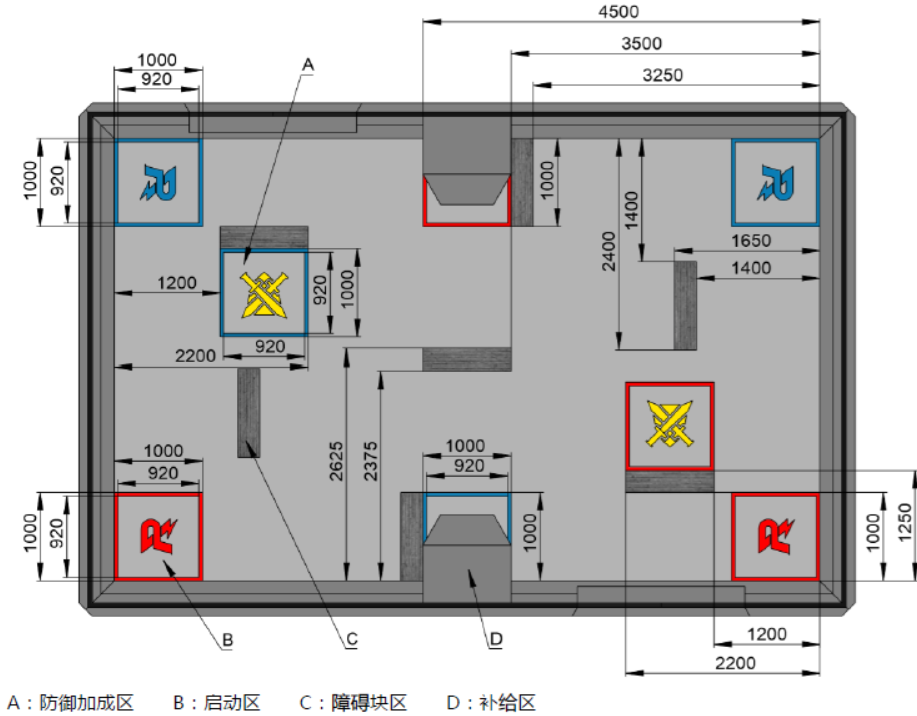
\includegraphics[width=\textwidth]{figures/field.png}
  \caption{挑战赛场地}\label{field}
\end{figure}

\begin{figure}[htb]
  \centering
  % Requires \usepackage{graphicx}
  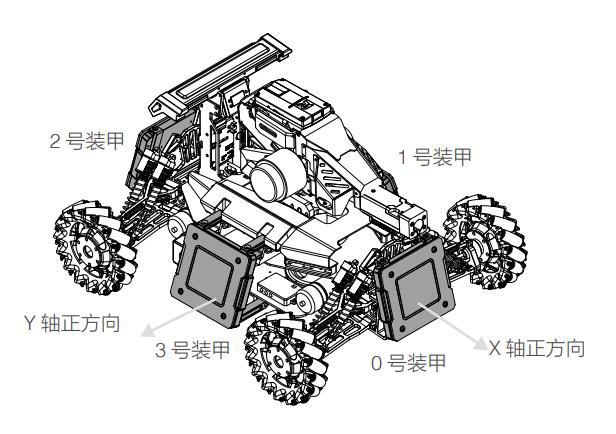
\includegraphics[width=\textwidth]{figures/robot.png}
  \caption{轮式机器人与装甲模块}\label{robot}
\end{figure}


敌我双方一到两台轮式机器人分别从各自图\ref{field}的B启动区启动,在挑战赛场地内进行全自主的对抗。在挑战赛场地内,设置诸多不可移动的灰色障碍物如图\ref{field}的C障碍块区所示。同时设置了A防御加成区,轮式机器人在这一区域中停留超过5s后即可获得伤害减半的buff持续时间30s。在D补给区己方轮式机器人可以获得弹药补给。

轮式机器人可以搭载激光雷达、摄像头、UWB、超声波等多种传感器。轮式机器人四周各装有装甲模块。装甲模块装有红蓝两种色彩的LED用以区别敌我,同时装有压力传感器以检测车身是否被击中,并计算剩余血量。装甲模块如图\ref{robot}所示。

\section{决策系统架构}
\subsection{架构概述}\label{system}
在应用与实践中,我们总结形成一套基于ROS的轮式机器人的控制软件系统。该架构包括该架构包括驱动模组、感知模组、规划模组、控制模组和决策模组。

驱动模组通过选取适合的驱动软件包调用摄像头、雷达、声呐、UWB等传感器数据以获取轮式机器人实时环境信息;通过解析步兵战车通信协议,构造串口驱动类,实现对轮式机器人的控制。感知模组通过雷达、声呐、UWB等传感器信息实现地图构建、实时定位;通过轻量级深度神经网络:SSD-MoblieNets达到了在Jetson TX2开发组件上的实时目标定位与追踪。规划模组主要通过优化Navigation功能包,实现了轻量级的路径规划器,使轮式机器人在有限的计算资源下,完成了全自主巡航功能。控制模组使用了离散式增量PID控制,其结合经典控制理论与SIMULINK仿真技术,实现了对目标物的低超调高速自动追踪。

\subsection{模组通信}
我们使用ROS的Publish/Subscribe机制实现各个模组之间的通信。各个模组的数据流如图\ref{dataflow}所示。各个ROS消息结点的消息传递关系如图\ref{topic}所示。

驱动模组负责将轮式机器人状态、比赛进度、电机里程计数据、摄像头图像、激光雷达云点阵、UWB定位等数据推送给感知模组。感知模组使用目标检测、物体识别与实时定位算法,确定当前己方轮式机器人与敌方轮式机器人在场地中的位置等状态信息。决策系统根据状态信息,将决策己方轮式机器人做出的反应动作,即目标位置与姿态,并将其推送给规划模组以经行路径规划。规划模组根据目标位置与姿态使用导航算法得出底盘与云台运动的速度等数据。这些数据由控制模组处理后,通过驱动模组中的串口驱动发送给下位机执行。

\begin{figure}[htb]
  \centering
  % Requires \usepackage{graphicx}
  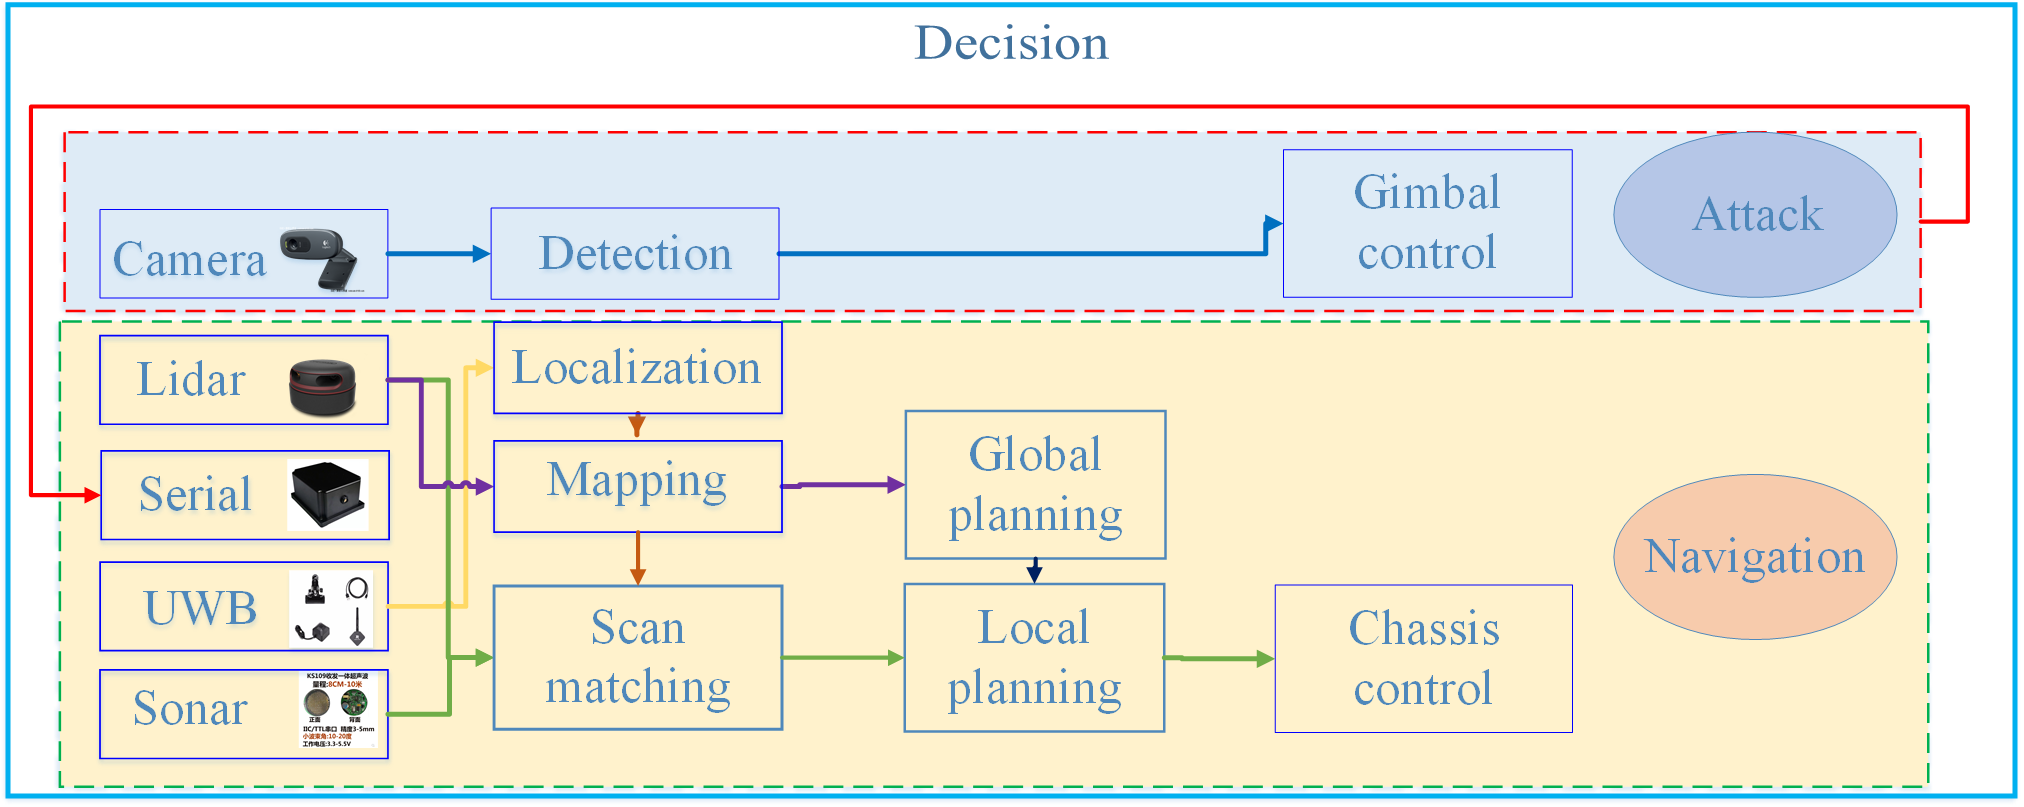
\includegraphics[width=\textwidth]{figures/dataflow.png}
  \caption{模组通信数据流}\label{dataflow}
\end{figure}

\begin{figure}[htb]
  \centering
  % Requires \usepackage{graphicx}
  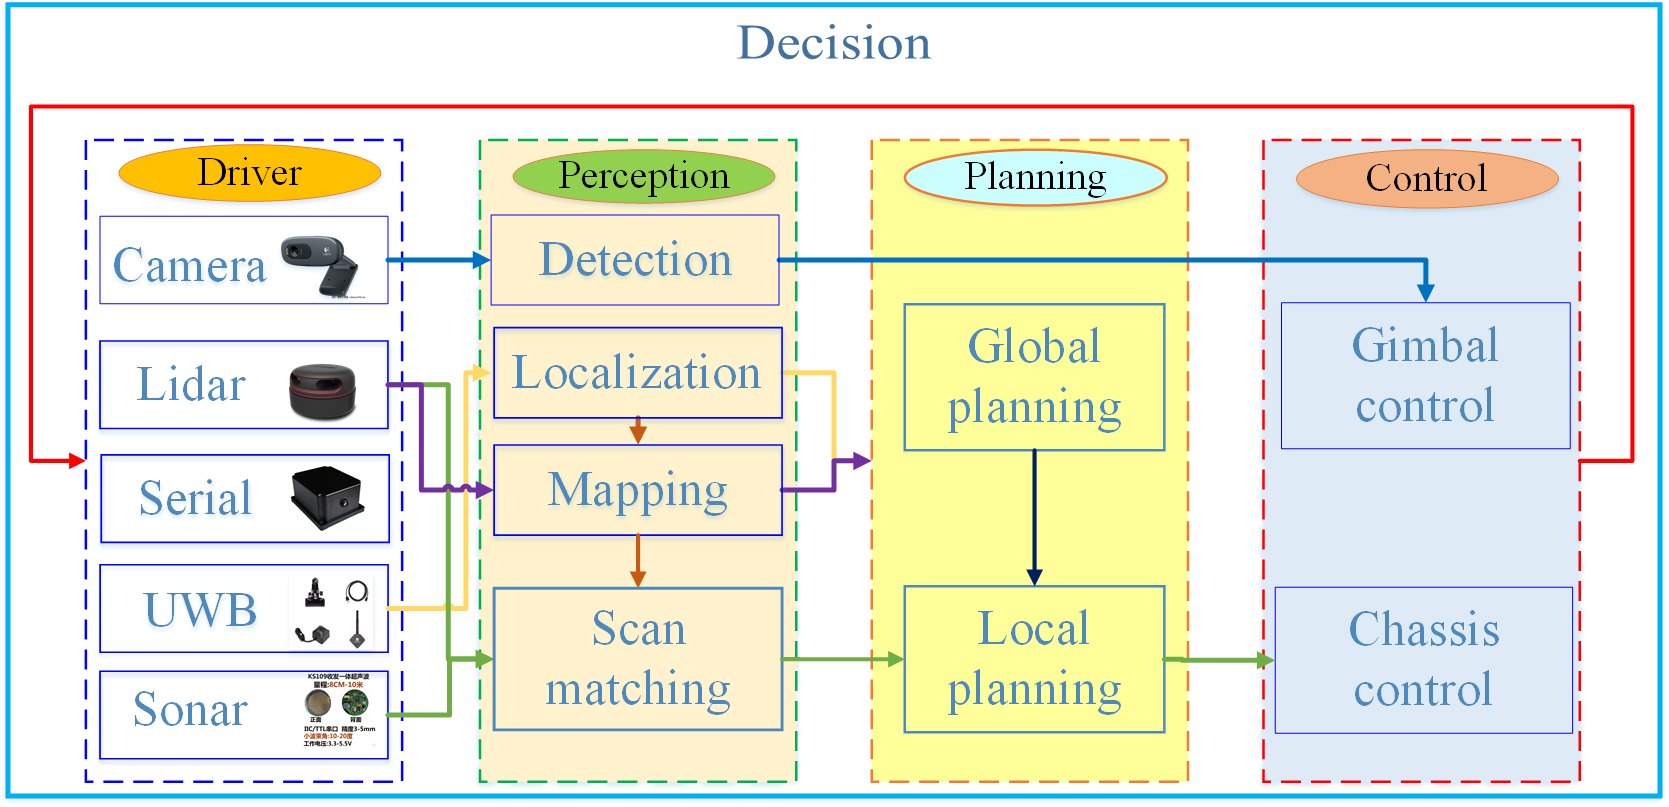
\includegraphics[width=\textwidth]{figures/function.png}
  \caption{模组功能}\label{function}
\end{figure}

\begin{figure}[htb]
  \centering
  % Requires \usepackage{graphicx}
  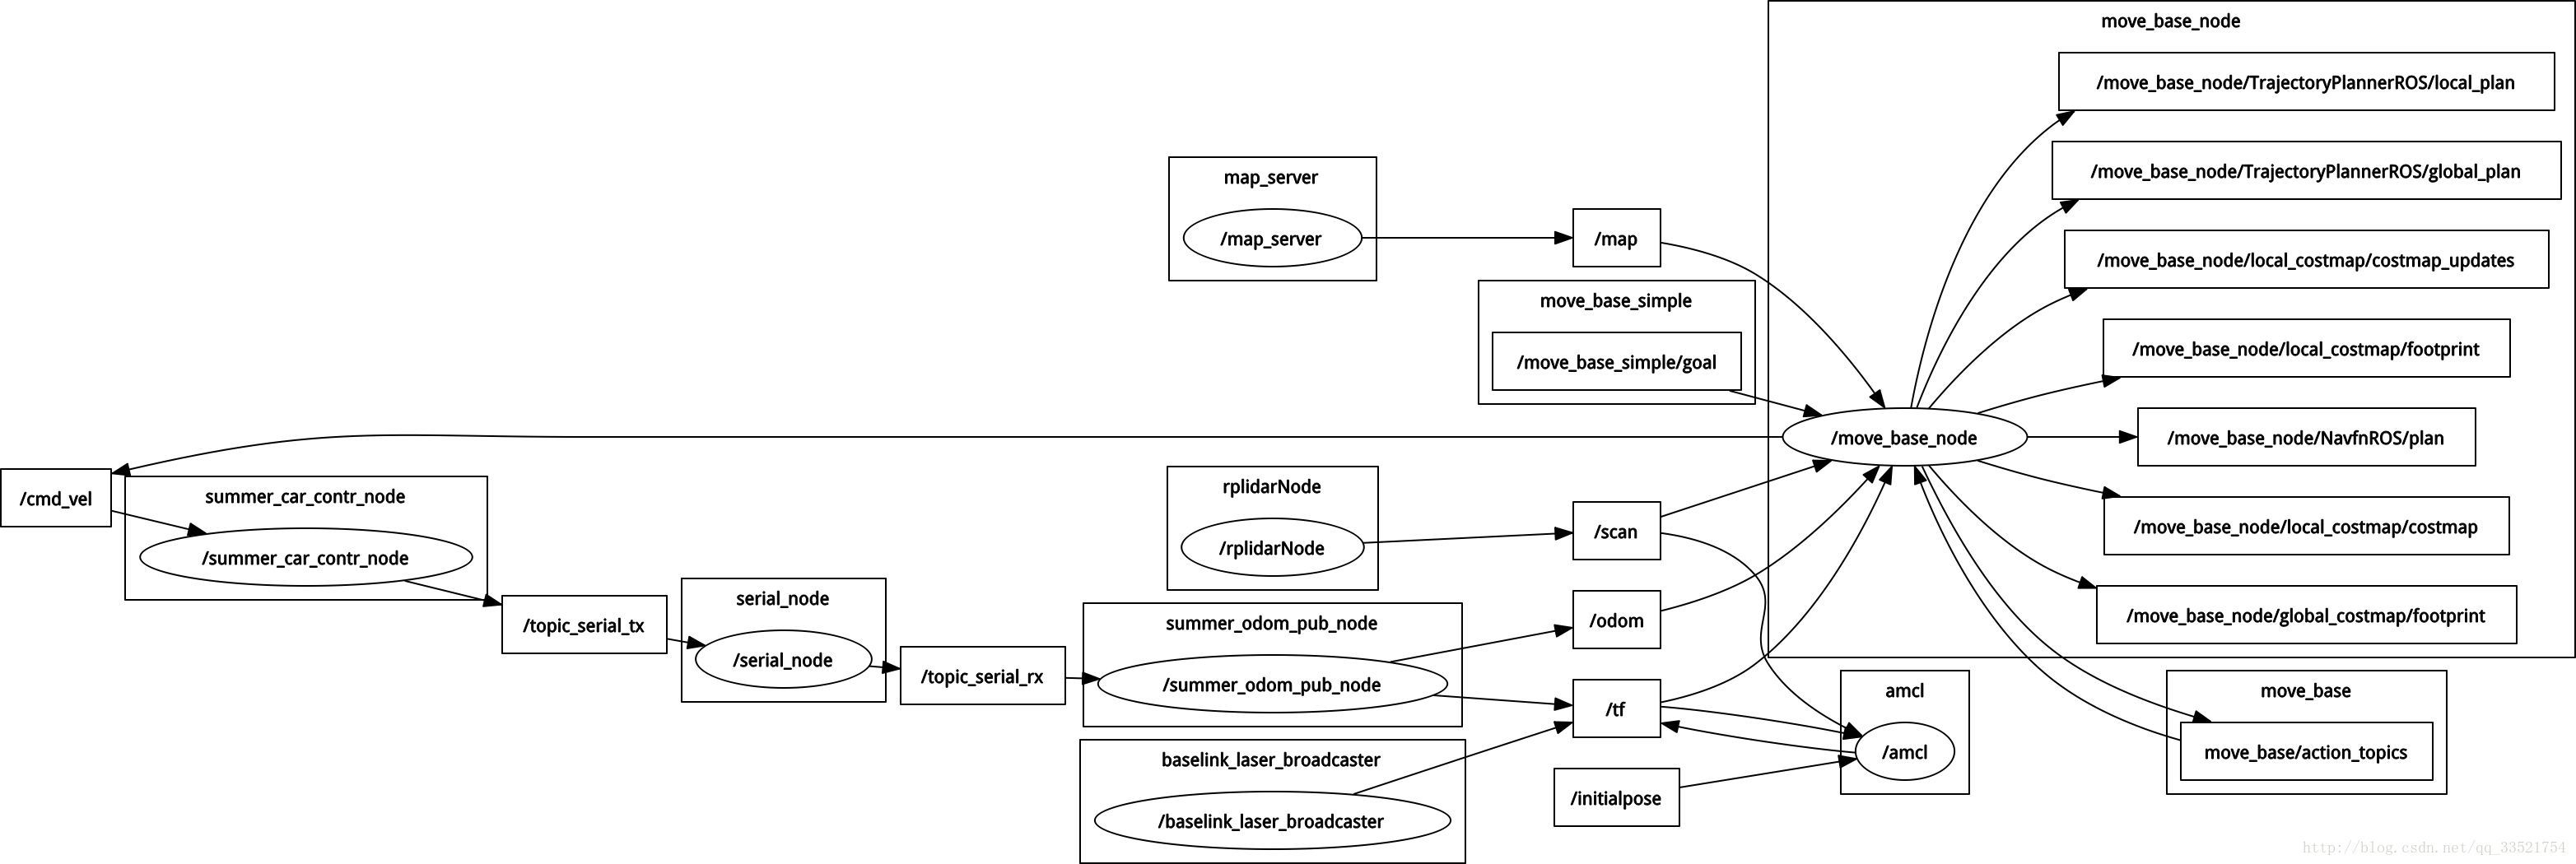
\includegraphics[width=\textwidth]{figures/topic.png}
  \caption{ROS消息结点关系}\label{topic}
\end{figure}

\subsection{模组功能}
总体而言,决策系统主要依赖改软件系统的两大功能:导航和攻击,如图\ref{function}所示。导航功能主要负责在挑战赛环境下自主避障、路径规划。攻击功能主要负责实时检测、追踪和打击敌方目标。决策系统建立在在可靠的导航与攻击功能上,实际上负责协调导航与攻击功能模块的交互。决策系统可以视为模组功能沟通与协调的结点,通过接收感知信息以合理地调用各个模组功能。

\section{决策系统设计}
在ROS平台上,决策系统实际上是一个消息处理结点,它通过处理轮式机器人的感知信息,向轮式机器人发布控制命令,已协调调用各个模组的功能,从而能够实现轮式机器人全自主的巡航、索敌、追踪与打击,如图\ref{decision} 所示。
\begin{figure}[htb]
  \centering
  % Requires \usepackage{graphicx}
  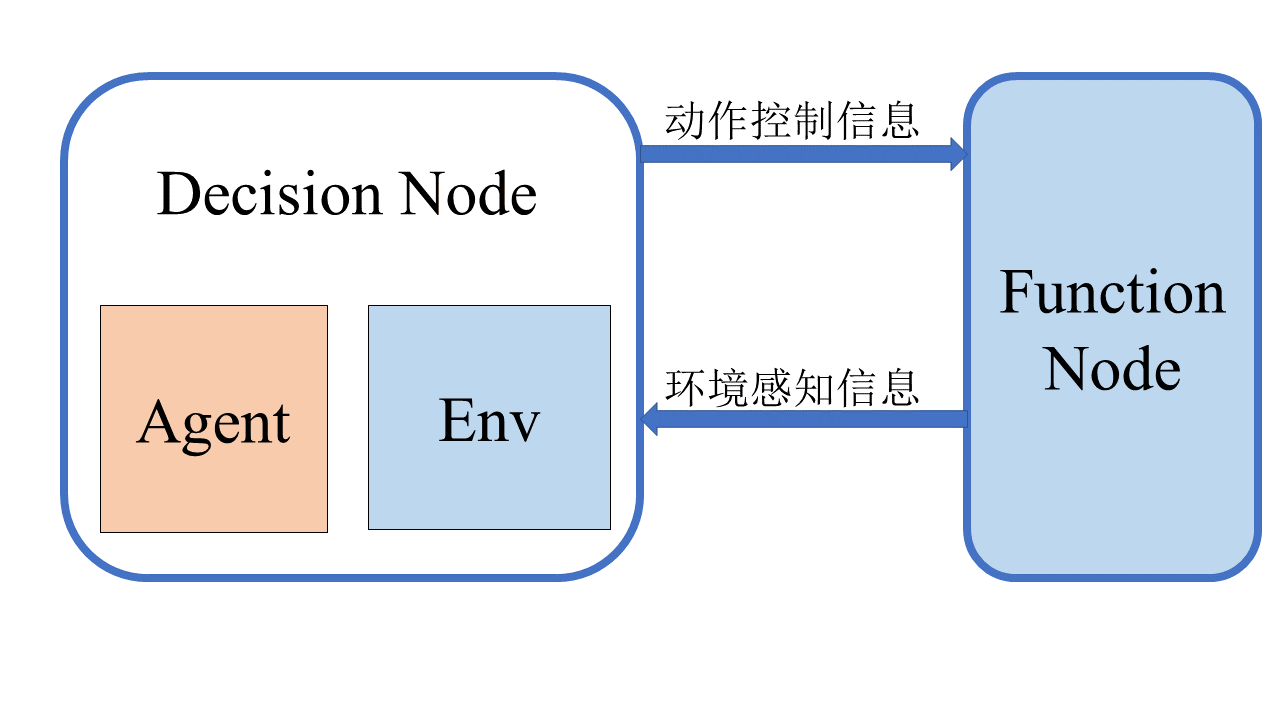
\includegraphics[width=\textwidth]{figures/decision.png}
  \caption{决策结点消息交互接口}\label{decision}
\end{figure}

在决策系统设计时,考虑到可扩展性、在虚拟环境与真实环境下的适应性、与深度强化学习算法的兼容性,我们使用OpenAI gym标准接口封装了轮式机器人感知、通信与控制功能,构建一个环境适配器类env,从而实现了智能体agent与环境env的交互。智能体agent通过状态state、动作action和奖励reward与环境env进行交互,从而进行训练,如图\ref{agentenv} 所示。
\begin{figure}[htb]
  \centering
  % Requires \usepackage{graphicx}
  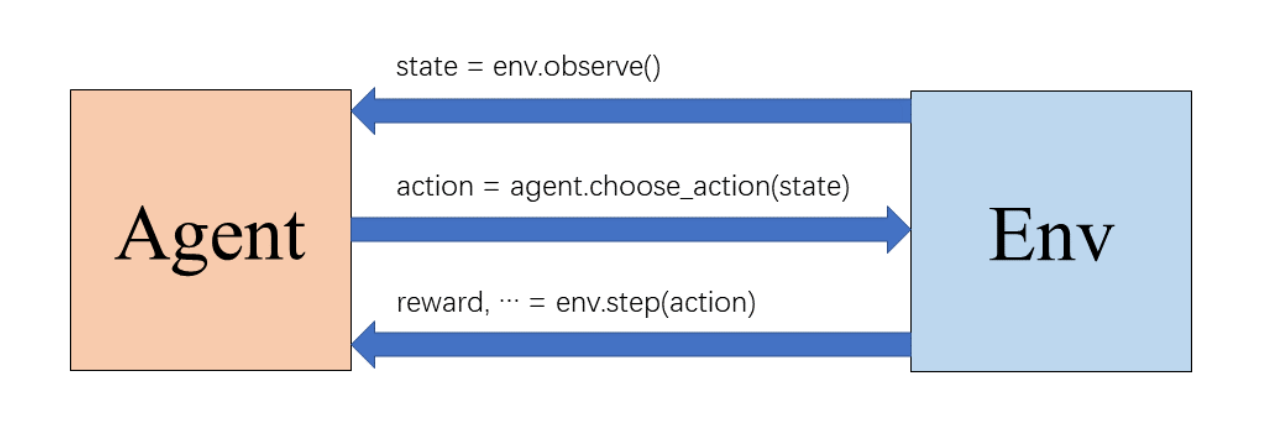
\includegraphics[width=\textwidth]{figures/agentenv.png}
  \caption{轮式机器人智能体与环境交互接口}\label{agentenv}
\end{figure}

按照OpenAI gym标准,我们将复杂的轮式机器人感知与控制抽象为智能体agent和环境env之间交互的三个函数:
\vspace{-10pt}
\begin{enumerate}
	\item 感知环境,$\text {env.observe}$。同步消息机制。输入为空,输出为轮式机器人智能体当前在环境中感知的状态。
	\item 动作决策,$\text {agent.choose action}$。同步消息机制。输入为轮式机器人智能体当前状态,输出为轮式机器人智能体自主做出的动作响应决策。
	\item 执行动作,$\text {env.step}$。同步消息机制。输入为轮式机器人智能体做出的动作响应,输出为环境反馈给轮式机器人智能体的奖励或惩罚和下一步。
\end{enumerate}

应用适配器模式的思想,将智能体agent做出动作决策与环境env交互解耦。环境env隐藏了决策系统结点与ROS目标识别、定位、移动控制等其他消息结点的交互细节,使智能体agent 只关心与环境env的交互。

环境env无需关心智能体agent的实现细节,通过继承env,可以是智能体在仿真轮式机器人环境与真是轮式机器人环境之间切换,从而提高了工作效率,减少了实验好耗时。

同样的,智能体agent无需关心环境env与轮式机器人的交互细节,通常来说,智能体agent只需要实现输入一个状态向量或矩阵$s$ 时,输出一个动作响应向量或矩阵$a$,就能够与环境env进行交互。因此,智能体agent可以在不同的强化学习算法、不同的神经网络模型之间灵活切换,甚至可以替换为非强化学习模型,如确定性有限状态机和行为树。

\subsection{确定性有限状态机}\label{dfa}
决策系统上我们使用人工设计的确定性有限状态机作为本文实验的基线,通过对所有可能出现的情况与相对应的行为来构建有限状态机,其中状态图如图\ref{state}所示,活动图如图\ref{activity} 所示,我们成功地对轮式机器人的行为策略进行规划,并在实际实践中取得良好的效果。

\begin{figure}[h]
  \centering
  % Requires \usepackage{graphicx}
  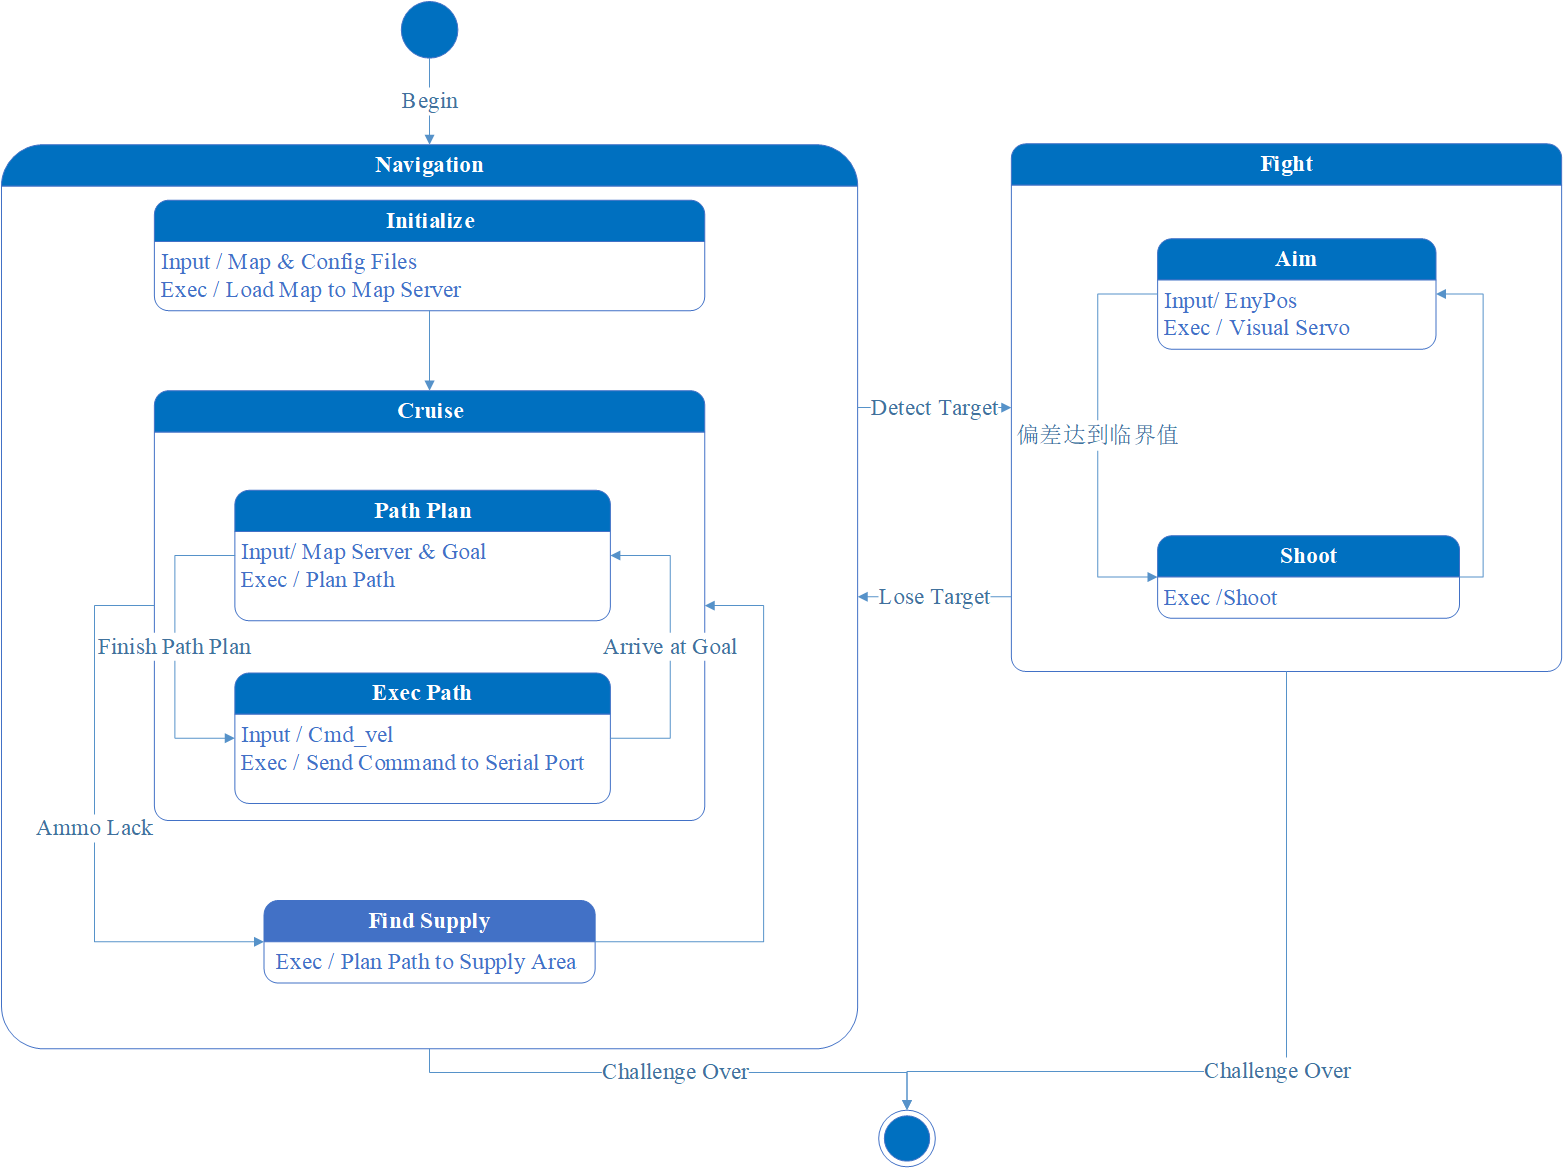
\includegraphics[width=\textwidth]{figures/state.png}
  \caption{轮式机器人确定性有限状态机}\label{state}
\end{figure}

\begin{figure}[h]
  \centering
  % Requires \usepackage{graphicx}
  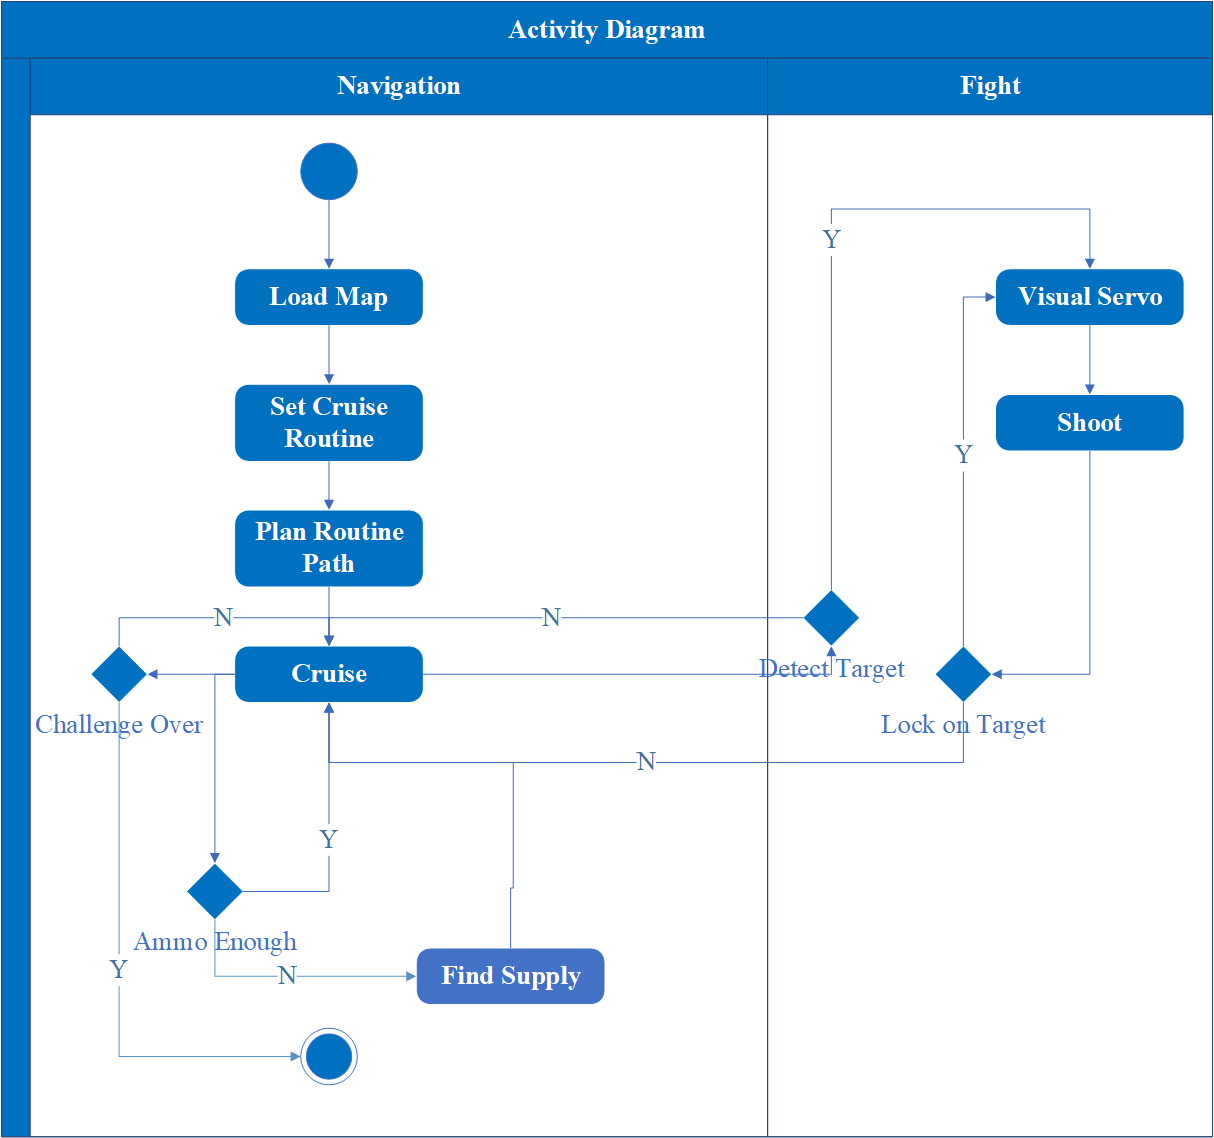
\includegraphics[width=\textwidth]{figures/activity.png}
  \caption{轮式机器人活动图}\label{activity}
\end{figure}

\chapter{强化学习算法研究与分析}\label{rl}

\section{强化学习基本原理}
强化学习的本质是通过与环境的交互进行学习。强化学习智能体与环境进行交互,并在观察到其行为的结果时,通过学习来改变自己的行为方式以响应所获得的奖励或惩罚。这种试错学习方法的范式来源于行为主义心理学,是强化学习的主要基础之一\cite{17}。另一个影响了强化学习的关键思想史最优控制,它提供了支撑该领域的数学形式。

在强化学习过程中,有机器学习算法控制的自主智能体在$t$时刻从环境中观察到状态$s_t$。智能体通过在状态$s_t$中执行动作$a_t$来与环境交互。当智能体执行动作时,环境和智能体将会根据当前的状态和所选择的动作转移到新的状态$s_{t+1}$。状态是对环境的充分统计数据,因此包括智能体采取最佳动作的所有必要信息,比如轮式机器人在环境中的位置。

最佳的动作顺序取决于环境提供的奖励。每次环境转换到新的状态时,它还会向智能体提供一个标量奖励$r_{t+1}$作为反馈。智能体的目标是学习一种最大化预期累加折扣的回报的策略。给定一个状态,策略返回要执行的动作,最优的策略就是能够最大化环境预期回报的策略。在这方面,强化学习旨在解决与最优控制相同的问题。然而,不像最优控制模型,强化学习中挑战的是智能体在不能获得状态转移的模型的情况下,通过反复试验来了解环境中行为的后果。与环境的每次交互都会产生信息,智能体会使用这些信息来更新其知识。这种感知、动作、学习的循环如图\ref{stateaction}所示。
\begin{figure}[htb]
  \centering
  % Requires \usepackage{graphicx}
  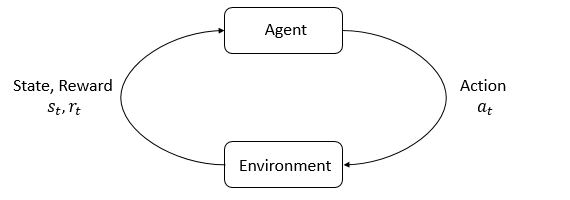
\includegraphics[width=0.80\textwidth]{figures/stateaction.png}
  \caption{强化学习基本模型}\label{stateaction}
\end{figure}

\subsection{马尔可夫决策过程}
强化学习过程可以用马尔可夫决策过程(MDP, Markov Decision Process)描述,它包含了以下定义:
\begin{itemize}
  \item $\mathcal{S}$,状态集合,包含一个初始状态分布$p \left( s_0 \right)$。
  \item $\mathcal{A}$,动作集合。
  \item $\mathcal{T}(s_{t+1}|s_t,a_t)$,状态转移函数,从$t$时刻的状态-动作对映射到$t+1$时的状态分布。
  \item $\mathcal{R}(s_t, a_t, s_{t+1})$,瞬时奖励。
  \item $\gamma \in [0,1]$,折扣参数,较低的折扣参数就会使模型更加重视瞬时奖励,较高的折扣参数则会使模型更加重视长期奖励。
\end{itemize}

通常来说,策略$\pi$定义了在特定时间特定状态下的行为方式,是一个从状态到每个可能的动作的概率的映射:$\pi : \mathcal{S} \to p(\mathcal{A} = a | \mathcal{S})$。$\pi(a_t|s_t)$就是指在状态$s_t$时选择执行动作$a_t$的概率。

在马尔可夫决策过程中,一个智能体从初始状态$s_0 \in \mathcal{S}$开始,在$t$时刻,观察到状态$s_t$,根据策略$\pi(a|s_t)$选择一个动作$a_t \in \mathcal{A}$执行,同时根据状态转移函数$\mathcal{T}(s|s_t,a_t)$,改变了智能体在环境中的状态到$s_{t+1} \in \mathcal{S}$,并使智能体获得奖励$r = \mathcal{R}(s_t, a_t, s_{t+1})$。z这一过程,如图\ref{mdp} 所示。

\begin{figure}[htb]
  \centering
  % Requires \usepackage{graphicx}
  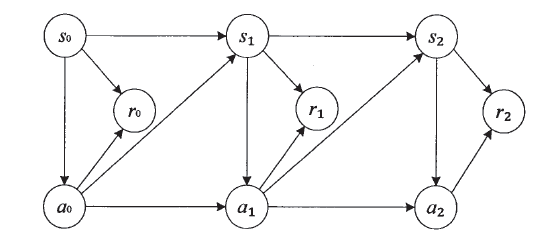
\includegraphics[width=0.80\textwidth]{figures/mdp.png}
  \caption{MDP动态过程}\label{mdp}
\end{figure}

对于情节性任务(Episodic Task),指状态会在时间$T$后结束并重置,以自然结束智能体(agent)和环境(environment)的交互,即所有任务可以被分解成一系列情节(episode),而情节的数目是有限的。那么在每一个情节中,状态、动作和奖励的序列就组成一个轨迹(trajectory)。一种策略中每一个轨迹所对应的瞬时奖励的折扣累加就是这个轨迹的回报(return)。
\begin{equation}
R = \sum_{k=0}^{T-1} \gamma^t r_{t+1}.
\end{equation}

对于连续性任务(Continuing Task),指任务不会自然结束,会一直持续到$T = \infty$。在这种情况下,我们使用$\gamma < 1$以保证累加奖励趋向于无穷。对于这种情况,我们不能计算一个完整轨迹的返回值,而是使用轨迹的一个有限子集。

强化学习的目标就是找到一个最优策略$\pi*$以最大化回报的期望。
\begin{equation}
\pi* = \text{argmax}_\pi \Bbb{E}[R|\pi].
\end{equation}

对于基于马尔可夫决策过程理论的强化学习来说,有一个重要的概念,那就是只有当前的状态会影响下一个状态,换而言之,在给定当前状态的情况下,未来状态与过去的状态是条件无关的。这意味着在状态$s_t$做出的任何动作决策只依赖于前一状态$s_{t-1}$\cite{18},而非${s_0, s_1, ..., s_{t-1}}$。即使这一假设被大多数强化学习方法采纳,但是这在本次实验的真实环境下是不现实的。因为这要求智能体的状态是能够被完全观察到的。

实际上当处于真实环境下,轮式机器人智能体只能观察到真实世界的部分状态。因此使用与马尔可夫决策过程的一般情况,部分可观测马尔可夫决策过程(POMDP)。在部分可观测马尔可夫决策过程中,智能体接收到一个观察结果(observation)$o_t \in \Omega$。观察结果是一个依赖于当前状态和先前动作的概率分布:$p(\o_{t+1}|s_{t+1},a_t)$。

在给定先前置信状态,采取的动作和当前的观察状态下,部分可观测马尔可夫决策过程通常维护一个对当前状态的置信度。深度学习中更常见的方法是利用递归神经网络(RNN, Recurrent Neural Network)。 它与前馈神经网络不同,是一个动态系统。当真实状态无法获知只能估计时,这种方法通过动态系统和状态空间模型解决了部分可观测马尔可夫决策过程。

\section{强化学习算法}
目前强化学习面临着许多挑战:
\begin{itemize}
  \item 强化学习必须通过与环境的反复实验来推断最优策略。智能体收到的唯一学习信号是奖励。
  \item 智能体的观察取决于其行为并且很可能包含强时间相关性。
  \item 智能体必须处理长时间的依赖关系。通常,一个动作的后果在环境状态进行多次转移后才会显现。
\end{itemize}

以轮式机器人你自主决策作战为例。如果目标位置已经确定,我们可能能够估计剩余的距离,并将其作为奖励信号,但我们不太可能确切地知道轮式机器人需要采取什么样的动作序列才能达到目标。由于轮式机器人必须在做出行进目标决策的同时导航,它的决策影响了它所能感知到的状态空间。最后,在导航了几个交叉路口后,轮式机器人可能会发现自己处于一条死路。从学习动作的后果到平衡探索与实践之间存在一系列问题,但这最终都可以来强化学习框架内解决。

根据是否基于模型,可以将强化学习算法分为基于模型学习(model-based learning)和模型无关学习(model-free learning)两种。

我们定义智能体学习和优化的策略称为目标策略,把智能体与环境进行实际交互行为的策略称为行为策略。根据智能体学习到的目标策略与智能体与实际环境交互的行为策略是否相同,我们将智能体分为同步策略学习(on-policy learning),又称在线学习和异步策略学习(off-policy learning),又称离线学习两种。

解决强化学习问题的方法主要分为两种:基于值函数的强化学习和基于策略搜索的强化学习。同时也有两种方法的混合,基于演员-评论家(actor-critic)模型的强化学习。

\subsection{值函数}
值函数方法基于估计所处状态的回报期望。状态值函数$V^{\pi}(s)$描述了处于状态$s$时,后续采取策略$\pi$的回报期望:
\begin{equation}
V^{\pi}(s) = \Bbb{E}[R|s,\pi].
\end{equation}

最优策略$\pi^*$对应的值函数$V*(s)$就是相应的最优值函数:
\begin{equation}
V^*(s) = \max_\pi V^{\pi}(s) \forall s \in \mathcal{S}.
\end{equation}

如果我们已经得到最优的值函数$V^*(s)$,最优策略$\pi^*$就可以通过回溯法得到。当智能体处于状态$s_t$时,在所有当前可以选择的动作中选择一个动作$a$最大化$\Bbb{E} _{s_{t+1} \sim \mathcal{T}(s_{t+1}|s_t,a)} [V^*(s_{t+1})]$。

在强化学习的过程中,状态转移函数$\mathcal{T}$是不可得的。因此,我们构建状态动作值函数$Q^\pi (s,a)$,即Q函数:
\begin{equation}
Q^{\pi}(s, a) = \Bbb{E} [R | s, a, \pi]
\end{equation}

在给定Q函数的情况下,最优策略可以通过在每一个状态下贪心选择动作$a = \text{argmax}_a Q^{\pi}(s, a)$来找到。在这种情况下,我们也可以定义$V^{\pi}(s)$,即$V^{\pi}(s) = \max_a Q^\pi (s,a)$。

为了实际学习$Q^\pi$,我们利用马尔可夫属性并将函数定义为Bellman方程,其具有以下递归形式:
\begin{equation}
Q^{\pi}(s_t, a_t) = \Bbb{E} [r_{t+1} + \gamma Q^\pi (s_{t+1}, \pi(s_{t+1}))].
\end{equation}

这意味着可以通过自助法(Bootstrapping)来优化$Q^\pi$,即我们可以使用对$Q^\pi$的估计的当前值来改进我们的估计。这是Q-learning\cite{19}和SARSA\cite{20}等算法的基础。

对于off-policy的Q-learning算法有:
\begin{equation}
Q^{\pi}(s_t, a_t) \leftarrow Q^{\pi}(s_t, a_t) + \alpha (r_t + \gamma \max_a Q^{\pi}(s_{t+1}, a)).
\end{equation}

对于on-policy的SARSA算法有:
\begin{equation}
Q^{\pi}(s_t, a_t) \leftarrow Q^{\pi}(s_t, a_t) + \alpha (r_t + \gamma Q^{\pi}(s_{t+1}, a_{t+1})).
\end{equation}

为了从任意$Q^\pi$中找到最优$Q^*$,我们使用广义策略迭代,其中策略迭代包括策略评估和策略改进。策略评估改进了值函数的估计,这可以通过最小化根据当前策略采取的路径产生的TD误差来实现。随着估计的改进,通过基于更新的值函数贪婪地选择动作,自然可以改善策略。通用策略迭代允许交错步骤,而不是单独地执行这些步骤以进行收敛,从而可以更快地进行。

\subsection{策略搜索}
策略搜索方法不需要维护值函数模型,而是直接搜索最优策略。通常选择参数化策略,之后使用基于梯度或无梯度的更新优化这些参数来最大化回报期望。使用神经网络对策略进行编码已经成功适用于无梯度和基于梯度的训练方法。无梯度优化可以有效地覆盖低维参数空间,尽管它们在应用于大型网络方面取得了一些成功\cite{21},但基于梯度的训练仍然是大多数深度强化学习的首选方法。当策略拥有大量参数时,基于梯度的训练的样本效率更高。

在直接构造策略时,通常输出概率分布的参数; 对于连续动作,这可以是高斯分布的均值和标准偏差,而对于离散动作,这可以是多项分布的个体概率。这样做的结果是一个可以直接采样动作的随机策略。使用无梯度方法,优化的策略则需要在预定义的模型类中进行启发式搜索。

\textbf{策略梯度(Policy Gradients):}对于如何改进参数化策略,梯度可以提供强有力的学习信号。然而,为了计算回报期望,我们需要对当前策略参数化引入的合理轨迹进行平均。这种平均需要确定性近似或通过采样的随机近似\cite{22}。确定性近似只能应用于基于模型的算法,其中可以获得状态转移函数的模型。在更常见的模型无关的R强化学习算法中,通常使用蒙塔卡罗方法估计回报期望。对于基于梯度的学习,这种蒙特卡罗近似提出了挑战,因为梯度不能通过随机函数的这些样本。因此,我们转向梯度的估计量,在强化学习中称为REINFORCE规则\cite{23}。REINFORCE规则可以用于计算随机变量$X$ 的函数$f$ 对于参数$\theta$ 的期望梯度:
\begin{equation}
\nabla_\theta \Bbb{E}_X [f(X;\theta)] = \Bbb{E}_X [f(X;\theta) \nabla_\theta \log p(X)].
\end{equation}

由于该计算依赖于轨迹的经验回归,因此得到的梯度具有高方差。通过引入噪声较小的无偏估计,可以减少方差。执行此操作的一般方法是减去基线,这意味着通过优势而不是纯回报来加权更新。

\textbf{演员-评论家(Actor-critic):}可以将值函数与策略的2显示表示相结合,从而产生演员-评论家方法,如图\ref{ac}所示。“演员”(策略)通过使用“评论家”(值函数)的反馈来学习。在这样做时,这些方法通过值函数方法的偏差引入来权衡策略梯度的方差减少\cite{23}\cite{24}。

演员-评论家方法使用值函数作为策略梯度的基线,因此演员-评论家方法与其他基线方法之间唯一的根本区别在于演员-评论家方法利用了一个优化过的值函数。
\begin{figure}[htb]
  \centering
  % Requires \usepackage{graphicx}
  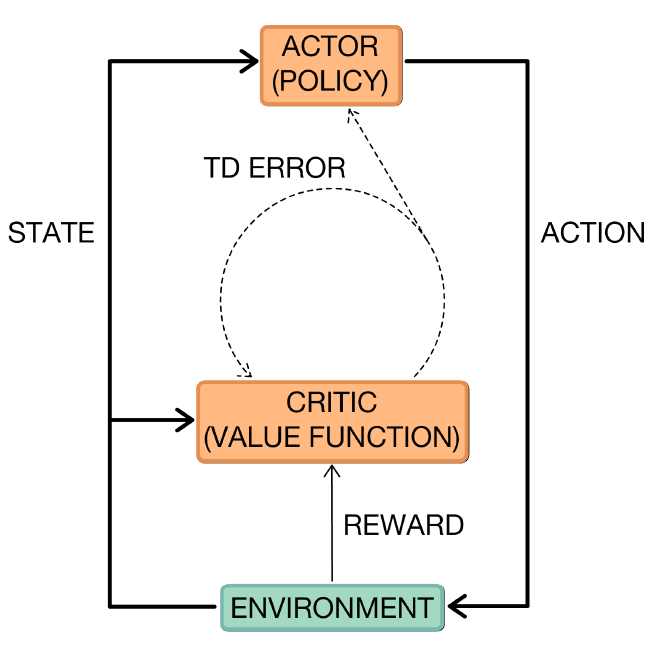
\includegraphics[width=0.80\textwidth]{figures/ac.png}
  \caption{演员-评论家(Actor-critic)方法}\label{ac}
\end{figure}

\subsection{深度强化学习}
深度强化学习的许多成功都是基于将强化学习的先前工作扩展到高维问题。这归功于低维特征学习和神经网络的强大函数逼近特性。通过特征学习,深度强化学习可以有效地处理维度灾难。例如,卷积神经网络(CNN, Convolutional Neural Network)可以用作强化学习智能体的组件,允许它们直接从原始的高维视觉输入中学习。通常,深度强化学习通过训练神经网络以近似最优策略$\pi^*$,或者最优值函数$V^*$,$Q^*$。

尽管当前深度强化学习成功使用无梯度的方法,但是绝大多数当前的工作依赖于梯度的反向传播算法。当可用时,梯度能够提供强大的学习信号。实际上,这些梯度是基于近似,通过采样或其他方式估计的,因此我们必须设计具有有效的归纳偏差的算法,以使它们易于处理。

反向传播的另一个好处是将回报期望的优化是为随机函数的优化。这个函数可以包含多个部分,包括模型、策略和值函数,通过各种方式组合。单个部分,例如值函数,可能不会直接优化回报期望,而是可以体现强化学习领域的有用信息。例如,使用可区分的模型和策略,可以在整个过程中进行前向传播和后向传播;另一方面,不确定性可能在很长一段时间内累积,此时使用值函数来总结统计数据可能是恰当的。我们之前已经提到特征学习和函数逼近是深度强化学习成功的关键,但也可以说深度学习领域激发了对强化学习的新思维方式。

\section{深度强化学习算法}
深度强化学习已经准备好在AI领域掀起一场革命。深度强化学习向建立对于真实世界具有高水平理解能力的全自主系统迈出了坚实的一步。当前,深度学习使强化学习有能力处理先前极为棘手的问题。深度强化学习也同样应用于机器人学领域,能够直接从真实世界摄像头的图片输入学习机器人控制策略。在本文中,我们首先介绍强化学习的通常概念,之后进一步阐述基于值和基于策略的方法。本文将覆盖深度强化学习的核心算法,包括DQN\cite{11}、DDPG\cite{26}、异步DDPG\cite{27}。同时,我们强调使用深度神经网络的优势,着重于关注于强化学习的理解。

\subsection{Deep Q-learning}
Deep Q-learning是第一个将深度学习模型与强化学习结合在一起从而成功地直接从高维的输入学习控制策略的算法。在Q-learning中使用Q值表来存储状态-动作对相应的Q值。然而当状态和动作空间是高维连续时,使用Q值表则不切实际。解决方法就是利用值函数近似,通过函数来近似Q值分布。借助深度神经网络来表示这个Q值函数就是DQN的核心思想。

通常DQN的实现中,会把收集的状态、动作、执行动作后的状态和奖励等信息存在内存中,训练的时候多次使用,称为回放记忆(replay memory)。注意到每个状态-动作对的Q值都要拟合,一个函数拟合自己可能引入额外的噪声,所以通常使用一个延迟更新的函数Q'来求新的Q值,称为目标值网络(target network),如图\ref{dqn}所示。如算法\ref{dqnalgorithm}所示。

DQN的改进包括Double DQN\cite{28}、Dueling DQN\cite{29}和Prioritized Replay\cite{30}。
Double DQN是在引入了target network后,改进Q值的计算方法,目的是减少因为Max Q值计算带来的计算偏差,或者称为过度估计问题。考虑到Q值和状态,动作都相关,但我们实际上更注重动作带来的奖励,Dueling DQN对网络结构做了改进。Prioritized Replay 探讨在回访记忆采样的优先级问题。

DQN以端到端的训练方式开创了深度强化学习对于高维输入的控制策略问题的解决方案。通过回放记忆解决相关性及非静态分布问题,使用目标值网络解决稳定性问题。但其在处理长时间的动作序列问题上仍然存在问题。

\begin{figure}[htb]
  \centering
  % Requires \usepackage{graphicx}
  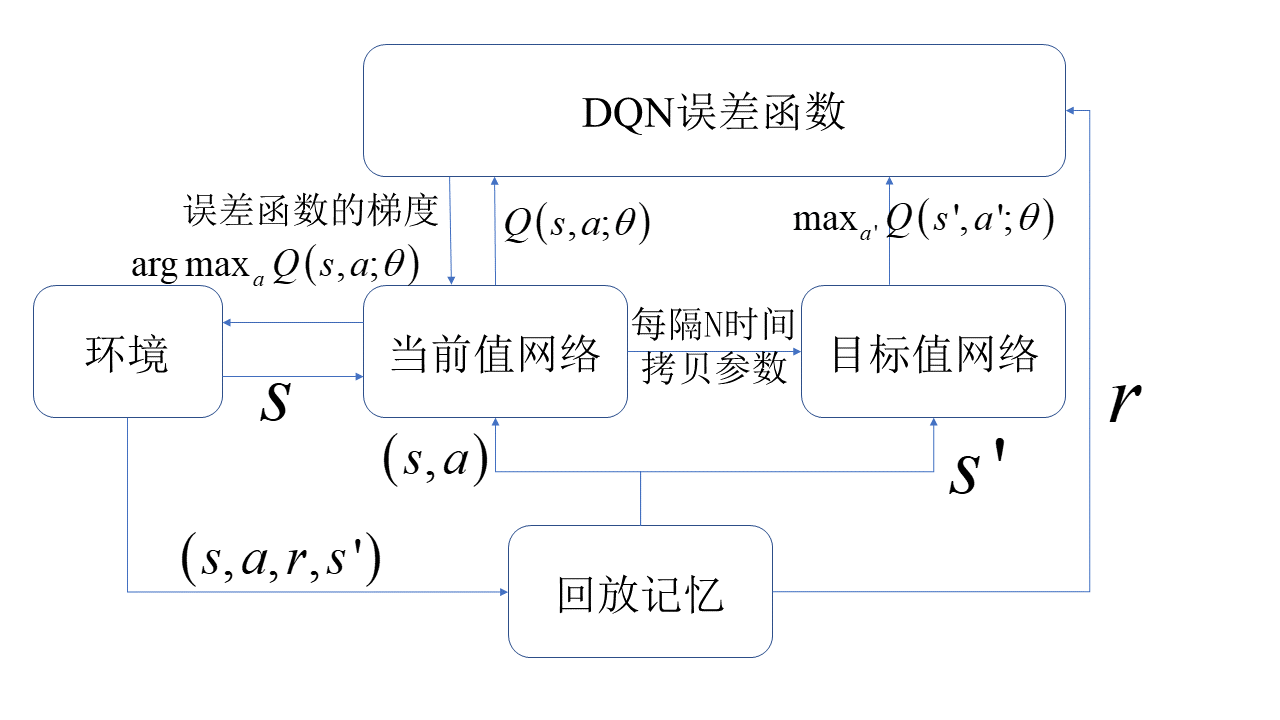
\includegraphics[width=\textwidth]{figures/DQN.png}
  \caption{DQN算法流程图}\label{dqn}
\end{figure}

\begin{algorithm}[htb]
\caption{Deep Q-learning}
\label{dqnalgorithm}
\begin{algorithmic}[1]
\State 初始化容量为$N$的回访记忆$\mathcal{D}$
\State 随机初始化动作值函数$Q$
\For{$\text{episode} = 1,M $}
    \State 初始化状态$s_1$
    \For{$t = 1, T$}
        \State 以概率$\epsilon$选择一个随机动作$a_t$
        \State 否则选择动作$a_t = \max_a Q^*(s_t,a;\theta)$
        \State 执行动作$a_t$得到奖励$r_t$并观察到环境$s_{t+1}$
        \State 保存$(s_t, a_t, r_t, s_{t+1})$到回放记忆$\mathcal{D}$
        \State 从回放记忆中采样一个minibatch$(s_t, a_t, r_t, s_{t+1})$
        \State 计算$y_j = \begin{cases} r_j,  & \text{$s_j$为终止状态} \\ r_j + \gamma \max_{a'} Q(s_{j+1}, a'; \theta), & \text{$s_{j+1}$不为终止状态}. \end{cases}$
        \State 计算$(y_j - Q(s_j, a_j; \theta))^2$的梯度下降并反向传播
    \EndFor
\EndFor
\end{algorithmic}
\end{algorithm}

\subsection{Deep Deterministic Policy Gradient}
深度确定性策略梯度(DDPG, Deep Deterministic Policy Gradient)是利用DQN扩展Q-learning算法的思路,对确定性策略梯度方法进行改造,基于前述演员-评论家框架的算法。该算法可用于解决连续动作空间上的深度强化学习问题。

DDPG中第一个D是深度神经网络,当概率策略的方差趋近于0的时候,就是确定性策略,其运用了Actor-Critic框架,把DQN和策略梯度混合了起来,显著提高样本利用率。如果动作空间也是连续的,那么就无法直接取到最大的Q值,那么我们再用个深度学习网络,称为演员Actor,演员的任务就是选Q值大的动作(确定性策略),演员的梯度来自值函数的估计网络(评论家),这个做法的最大优势是,能够离线地更新策略,即像DQN一样,从回放记忆采样出数据来训练,如图\ref{ddpg}所示。区别于DQN,DQN每隔一定的迭代次数后,将参数复制给实现网络;而DDPG中目标网络的参数每次迭代都以微小量逼近实现网络的参数。

在DDPG中,分别使用参数为$\theta^\mu$和$\theta^Q$的深度神经网络来表示确定性策略$a = \pi(s|\theta^\mu)$和动作值函数$Q(s,a|\theta^Q)$。其中,策略网络用来更新策略,对应演员;智网络用来逼近状态动作对的值函数,并提供梯度信息,对应评论家。目标函数被定义为带折扣的回报期望。
\begin{equation}
J(\theta^\mu) = \Bbb{E}_{\theta^\mu}[\sum_{t=0}^T \gamma^t r_{t+1}].
\end{equation}

通过随机梯度法对目标函数进行端到端的优化。目标函数关于$\theta^\mu$的梯度等价于Q值函数关于$\theta^\mu$的期望梯度:
\begin{equation}
\frac{\partial J(\theta^\mu)} {\partial \theta^\mu} = \Bbb{E}_s[\frac{\partial Q(s, a | \theta^Q)}{\partial \theta^\mu}].
\end{equation}

根据确定性策略$a = \pi(s|\theta^\mu)$,可得
\begin{equation}
\frac{\partial J(\theta^\mu)} {\partial \theta^\mu} = \Bbb{E}_s[\frac{\partial Q(s, a | \theta^Q)}{\partial a}\frac{\partial \pi(s|\theta^\mu)}{\partial \theta^\mu}].
\end{equation}

沿着提升Q值的方向更新策略网络的参数。

通过DQN中更新网络的方式来更新评论家网络,梯度信息为:
\begin{equation}
\frac{\partial L(\theta^Q)} {\partial \theta^Q} = \Bbb{E}_{s,a,r,s' \sim \mathcal{D}} [(r + \gamma Q'(s',\pi(s'|\theta^{\mu'})|\theta^{Q'}) - Q(s,a|\theta^Q)) \frac{\partial Q(s,a|\theta^Q)}{\partial \theta^Q}]
\end{equation}

如算法\ref{ddpgalgorithm}所示。

\begin{figure}[htb]
  \centering
  % Requires \usepackage{graphicx}
  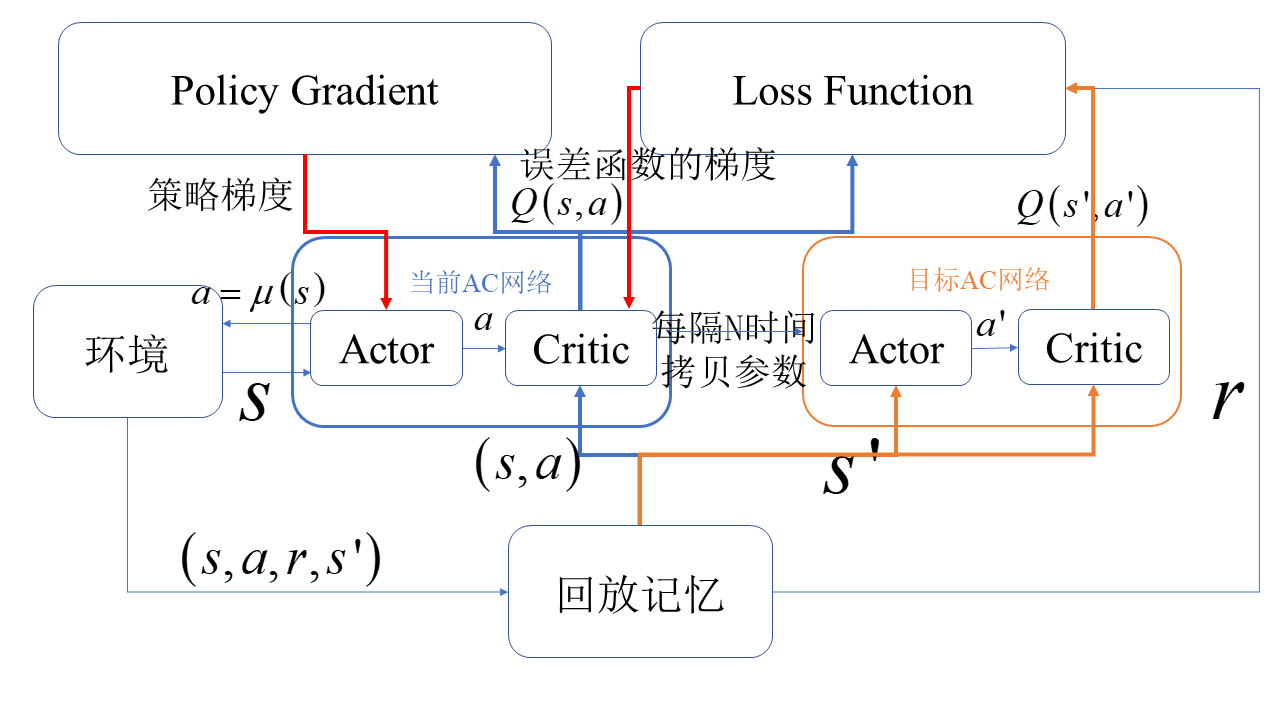
\includegraphics[width=\textwidth]{figures/ddpg.png}
  \caption{DDPG算法流程图}\label{ddpg}
\end{figure}

\begin{algorithm}[htb]
\caption{Deep Deterministic Policy Gradient}
\label{ddpgalgorithm}
\begin{algorithmic}[1]
\State 以随机参数$\theta^Q$和$\theta^\mu$初始化评论家网络$Q(s,a|\theta^Q)$和演员策略$\mu(s|\theta^\mu)$
\State 初始化容量为$N$的回访记忆$\mathcal{D}$
\For{$\text{episode} = 1,M $}
    \State 初始化状态$s_1$
    \State 初始化一个计算过程$\mathcal{N}$
    \For{$t = 1, T$}
        \State 选择动作$a_t = \mu(s_t|\theta^\mu) + \mathcal{N}_t$
        \State 执行动作$a_t$得到奖励$r_t$并观察到环境$s_{t+1}$
        \State 保存$(s_t, a_t, r_t, s_{t+1})$到回放记忆$\mathcal{D}$
        \State 从回放记忆中采样一个minibatch$(s_t, a_t, r_t, s_{t+1})$
        \State 计算$y_j = \begin{cases} r_j,  & \text{$s_j$为终止状态} \\ r_j + \gamma Q(s_{j+1}, \mu'(s_{i+1}|\theta^{\mu'}); \theta^{Q'}), & \text{$s_{j+1}$不为终止状态}. \end{cases}$
        \State 减小损失以更新评论家:$L = \frac{1}{N}\sum_j ((y_j - Q(s_j, a_j; \theta^Q))^2)$
        \State 使用策略梯度以更新演员:$\nabla_{\theta^\mu} J \approx \frac{1}{N} \sum_i \nabla_a Q(s,a|\theta^Q)|_{s=s_i,a=\mu(s_i)} \nabla_{\theta^\mu} \mu(s|\theta^\mu)$
    \EndFor
\EndFor
\end{algorithmic}
\end{algorithm}

DDPG不仅在一系列连续动作空间的任务中表现稳定,而且求得最优解所需要的时间步也远远少于DQN。与基于值函数的深度强化学习方法相比,基于演员-评论家框架的深度策略梯度方法优化策略效率更高,求解速度更快。

\subsection{多智能体异步DDPG}
与虚拟环境相比,在真实环境中,深度强化学习在轮式机器人上的训练面临以下挑战:
\begin{itemize}
  \item 在虚拟环境下训练深度强化学习时,可以通过读取一帧状态后暂停模拟器,训练网络后再启动模拟器执行动作。而在真实环境下的轮式机器人控制是一个要求强实时性的问题。当读取一帧状态还未选择动作时,状态可能已经发生了变换,这就不满足马尔可夫决策过程。
  \item 在虚拟环境下可以对环境变化的模拟进行加速,而真实环境下的轮式机器人不可能做到,这就造成了采样速度非常缓慢。
  \item 在虚拟环境下可以不用考虑轮式机器人的安全问题,在真实环境下则需要对轮式机器人的动作空间做出一系列的限制。
\end{itemize}

频繁的使轮式机器人暂停以排除网络训练时延是不现实的:
\begin{enumerate}
  \item 首先,这对于轮式机器人的控制电路、电机与制动装置造成大量的损耗。
  \item 其次,若想在训练时延期间,保持轮式机器人状态不变,则同时需要关停敌我双方所有轮式机器人,则需要建立敌我双方的通信机制。这在挑战赛规则中是不允许的,同时也丧失了决策系统的存在意义。
  \item 最后,频繁的暂停一定会拖慢采集训练样本的速度。
\end{enumerate}

因此我们采取多智能体异步训练,即多个轮式机器人作为收集线程负责收集样本,一个训练线程负责训练网络,如算法\ref{amalgorithm}所示。在收集样本运行的每一个episode中,初始化时从训练线程同步策略网络,每一步结束后,将状态、动作、奖励等存入共享的回放记忆中。这样使得在真实环境中的轮式机器人能够不受网络训练时延的困扰,同时成倍的加快训练数据采样的速度。除此之外,通过设置不同的动作参数,如不同贪心策略系数$\epsilon$和随机噪声$\mathcal{N}$可以使模型更具稳健性。

\begin{algorithm}[ht]
\caption{多智能体异步DDPG}
\label{amalgorithm}
\begin{algorithmic}[1]

\State // 训练线程
\State 以随机参数$\theta^Q$和$\theta^\mu$初始化评论家网络$Q(s,a|\theta^Q)$和演员策略$\mu(s|\theta^\mu)$
\State 初始化容量为$N$的回访记忆$\mathcal{D}$
\For{$\text{iteration} = 1, I $}
    \State 从回放记忆中采样一个minibatch$(s_t, a_t, r_t, s_{t+1})$
    \State 计算$y_j = \begin{cases} r_j,  & \text{$s_j$为终止状态} \\ r_j + \gamma Q(s_{j+1}, \mu'(s_{i+1}|\theta^{\mu'}); \theta^{Q'}), & \text{$s_{j+1}$不为终止状态}. \end{cases}$
    \State 减小损失以更新评论家:$L = \frac{1}{N}\sum_j ((y_j - Q(s_j, a_j; \theta^Q))^2)$
    \State 使用策略梯度以更新演员:$\nabla_{\theta^\mu} J \approx \frac{1}{N} \sum_i \nabla_a Q(s,a|\theta^Q)|_{s=s_i,a=\mu(s_i)} \nabla_{\theta^\mu} \mu(s|\theta^\mu)$
\EndFor

\State // 收集线程$n, n=1...N$
\State 以随机参数$\theta^\mu_n$初始化评演员策略$\mu(s|\theta^\mu_n)$
\For{$\text{episode} = 1,M $}
    \State 同步策略网络权重$\theta^\mu_n \leftarrow \theta_mu$
    \State 初始化状态$s_1$
    \State 初始化一个计算过程$\mathcal{N}$
    \For{$t = 1, T$}
        \State 选择动作$a_t = \mu(s_t|\theta^\mu_n) + \mathcal{N}_t$
        \State 执行动作$a_t$得到奖励$r_t$并观察到环境$s_{t+1}$
        \State 保存$(s_t, a_t, r_t, s_{t+1})$到回放记忆$\mathcal{D}$
    \EndFor
\EndFor

\end{algorithmic}
\end{algorithm}

\chapter{实验数据采集与分析}\label{experiment}

\section{仿真平台}
\subsection{ROS简介}
ROS(Robot Operating System,机器人操作系统)是为机器人软件开发的一种计算机操作系统架构,源自于斯坦福AI机器人项目。ROS能够为跨平台、跨语言的异构计算机集群提供结构化通信。ROS包括标准的操作系统环境,包括底层设备控制与管理、进程间消息传递机制和软件包管理等功能。ROS操作系统能够使开发者非常方便的构建多语言的机器人软件功能。如\ref{system} 所述,我们在ROS系统的基础上构建驱动、感知、规划、控制和决策功能模组。

\subsection{RVIZ与Gazebo}
RVIZ是ROS自带的图形化工具。在本文中,我们将轮式机器人的雷达、里程计等传感器数据以及定位、路径规划等感知和规划功能模组中间结果在RVIZ界面中进行可视化,如图\ref{rviz}所示。Gazebo是基于ROS的一款功能强大的3D 机器人仿真模拟器。我们使用Gazebo进行仿真建模,准确有效地模拟复现轮式机器人在挑战赛场地内的状态和行为,如图\ref{gazebo}所示。Gazebo通过高性能的物理引擎,对轮式机器人进行物理建模,动力学仿真,模拟真实环境下的传感器和噪声,使我们的强化学习算法获得逼近于真实环境的训练。
\begin{figure}[ht]
  \centering
  % Requires \usepackage{graphicx}
  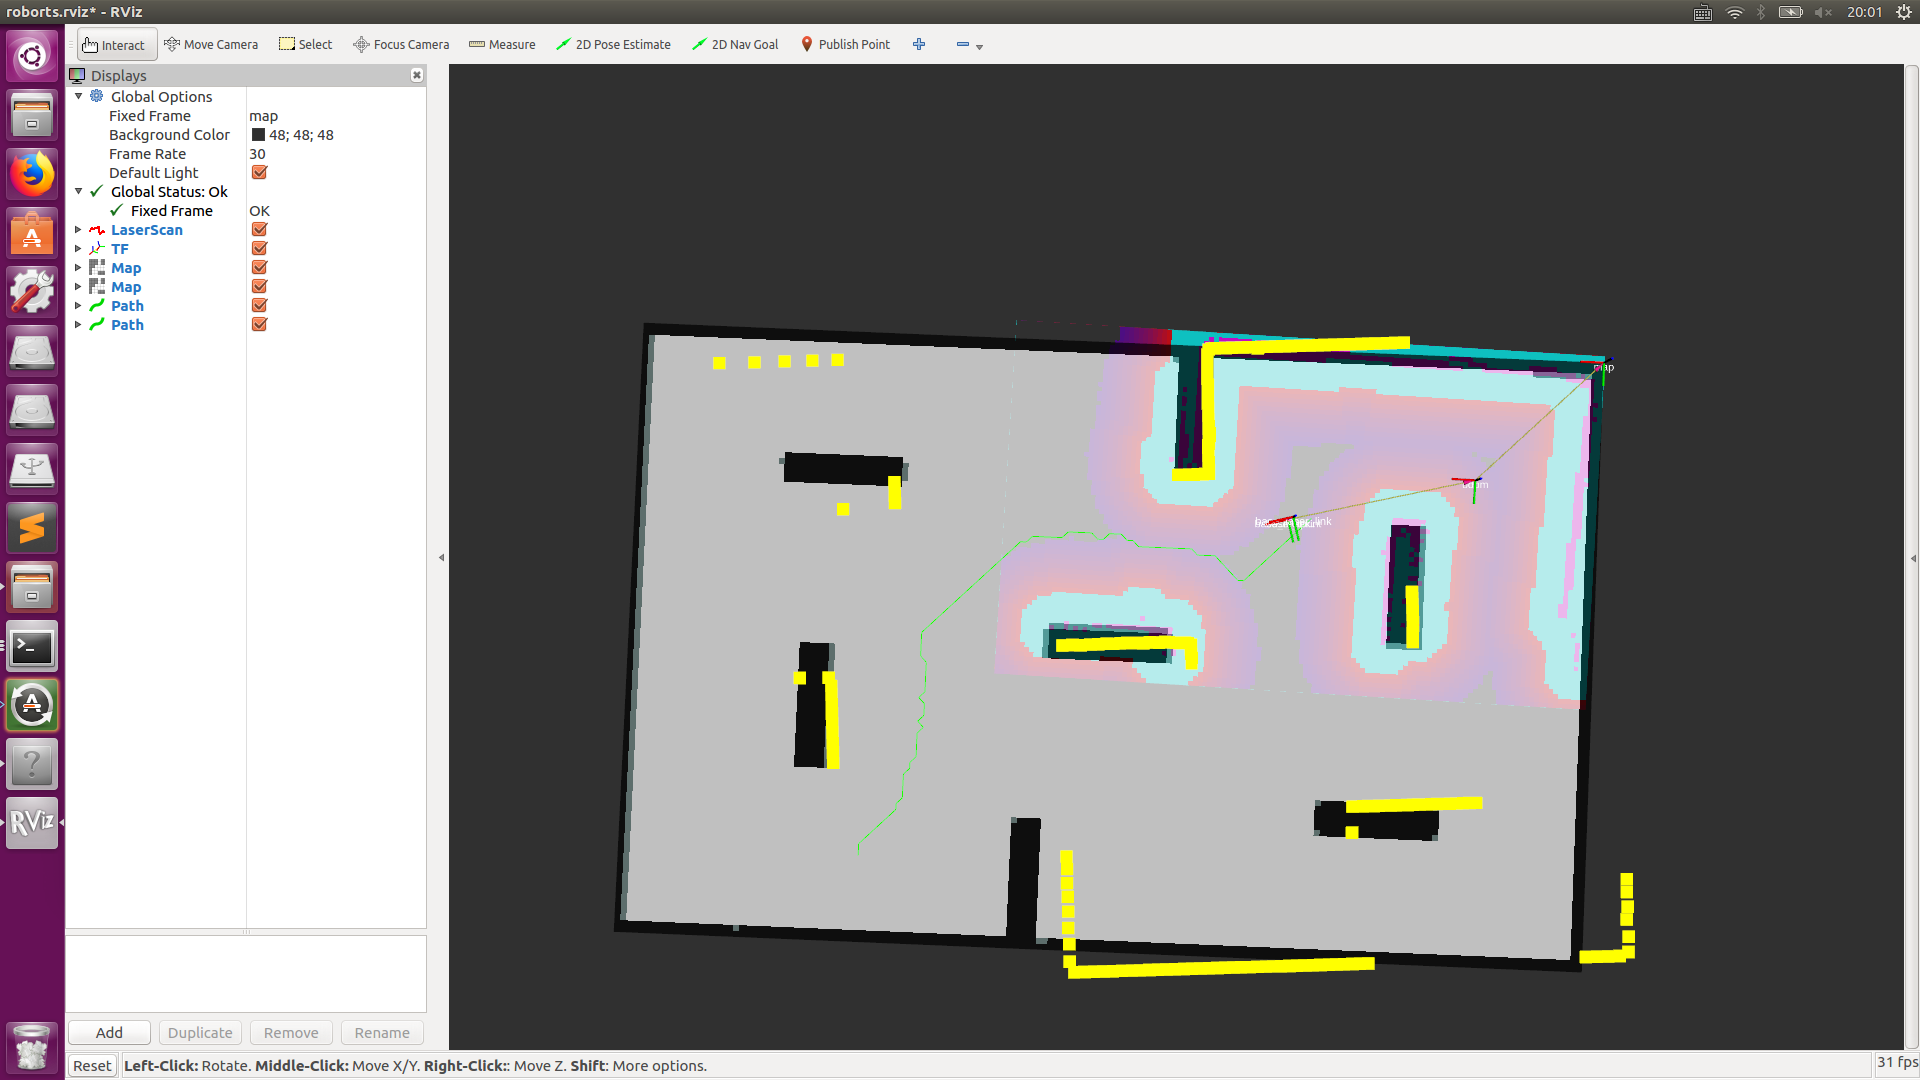
\includegraphics[width=0.80\textwidth]{figures/rviz.jpg}
  \caption{RVIZ界面}\label{rviz}
\end{figure}

\begin{figure}[ht]
  \centering
  % Requires \usepackage{graphicx}
  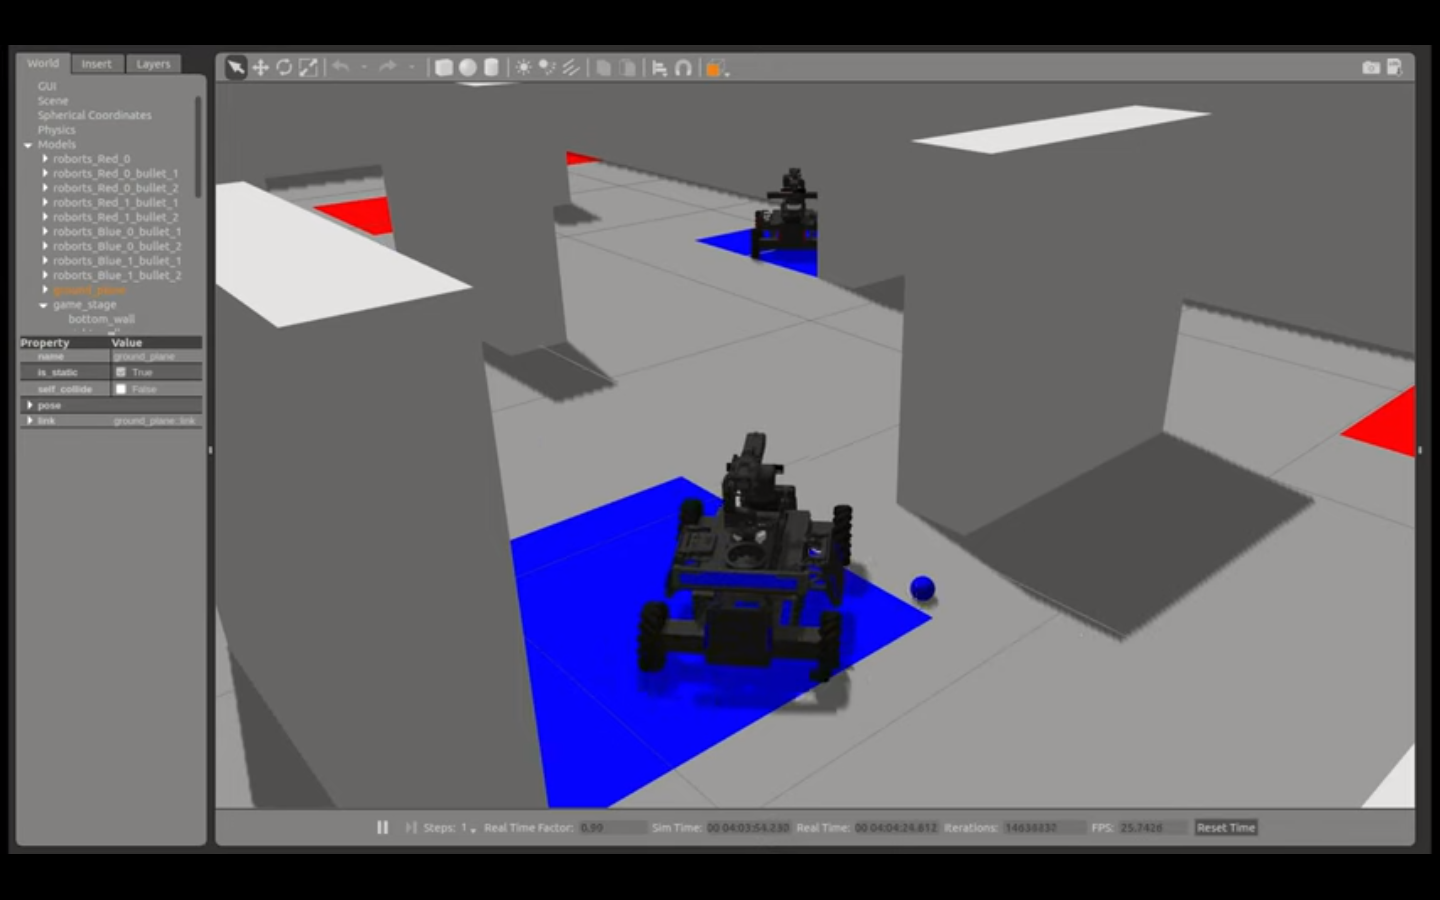
\includegraphics[width=0.80\textwidth]{figures/gazebo.png}
  \caption{Gazebo物理仿真}\label{gazebo}
\end{figure}

\section{真实环境}
我们在真实环境中使用的轮式机器人如图\ref{realrobot}所示。在真实环境中的深度强化学习训练具有比在虚拟环境下训练更具挑战性的问题:
\begin{enumerate}
  \item 必须选择适当的策略或者值函数表示,以便实现对物理硬件实用的训练时间。
  \item 必须提供实例演示来初始化策略并减轻训练期间的安全问题。
  \item 必须考虑到轮式机器人在真实世界的感知、通信和控制时延。
\end{enumerate}

针对安全问题,我们在进行真实环境下的实验时,进行一下设置以保证训练过程安全有效:
\begin{enumerate}
  \item 训练时,靶车即敌方机器人由人类操作员操作,以保证轮式机器人与场地人员安全。进行测试时,靶车由如图\ref{state}所示的确定性有限状态机控制作为实验基线。
  \item 训练时,轮式机器人在硬件上设置安全阈值和异常中断阈值,如表\ref{safty}。核查控制代码,使其控制论机器人的过程中,各安全项目的理论值在安全阈值以内。创建一个ROS结点,轮询安全项目数值,如果有超过异常中断阈值,则记录异常数值并终止轮式机器人运动。
  \item 训练时,使用远程桌面VNC控制轮式机器人。除操作员以外,无关人员禁止进入训练场地。
\end{enumerate}

针对时延问题,我们使用多智能体异步训练方法以求轮式机器人智能体能够克服物理时延带来的问题。

\begin{figure}[ht]
  \centering
  % Requires \usepackage{graphicx}
  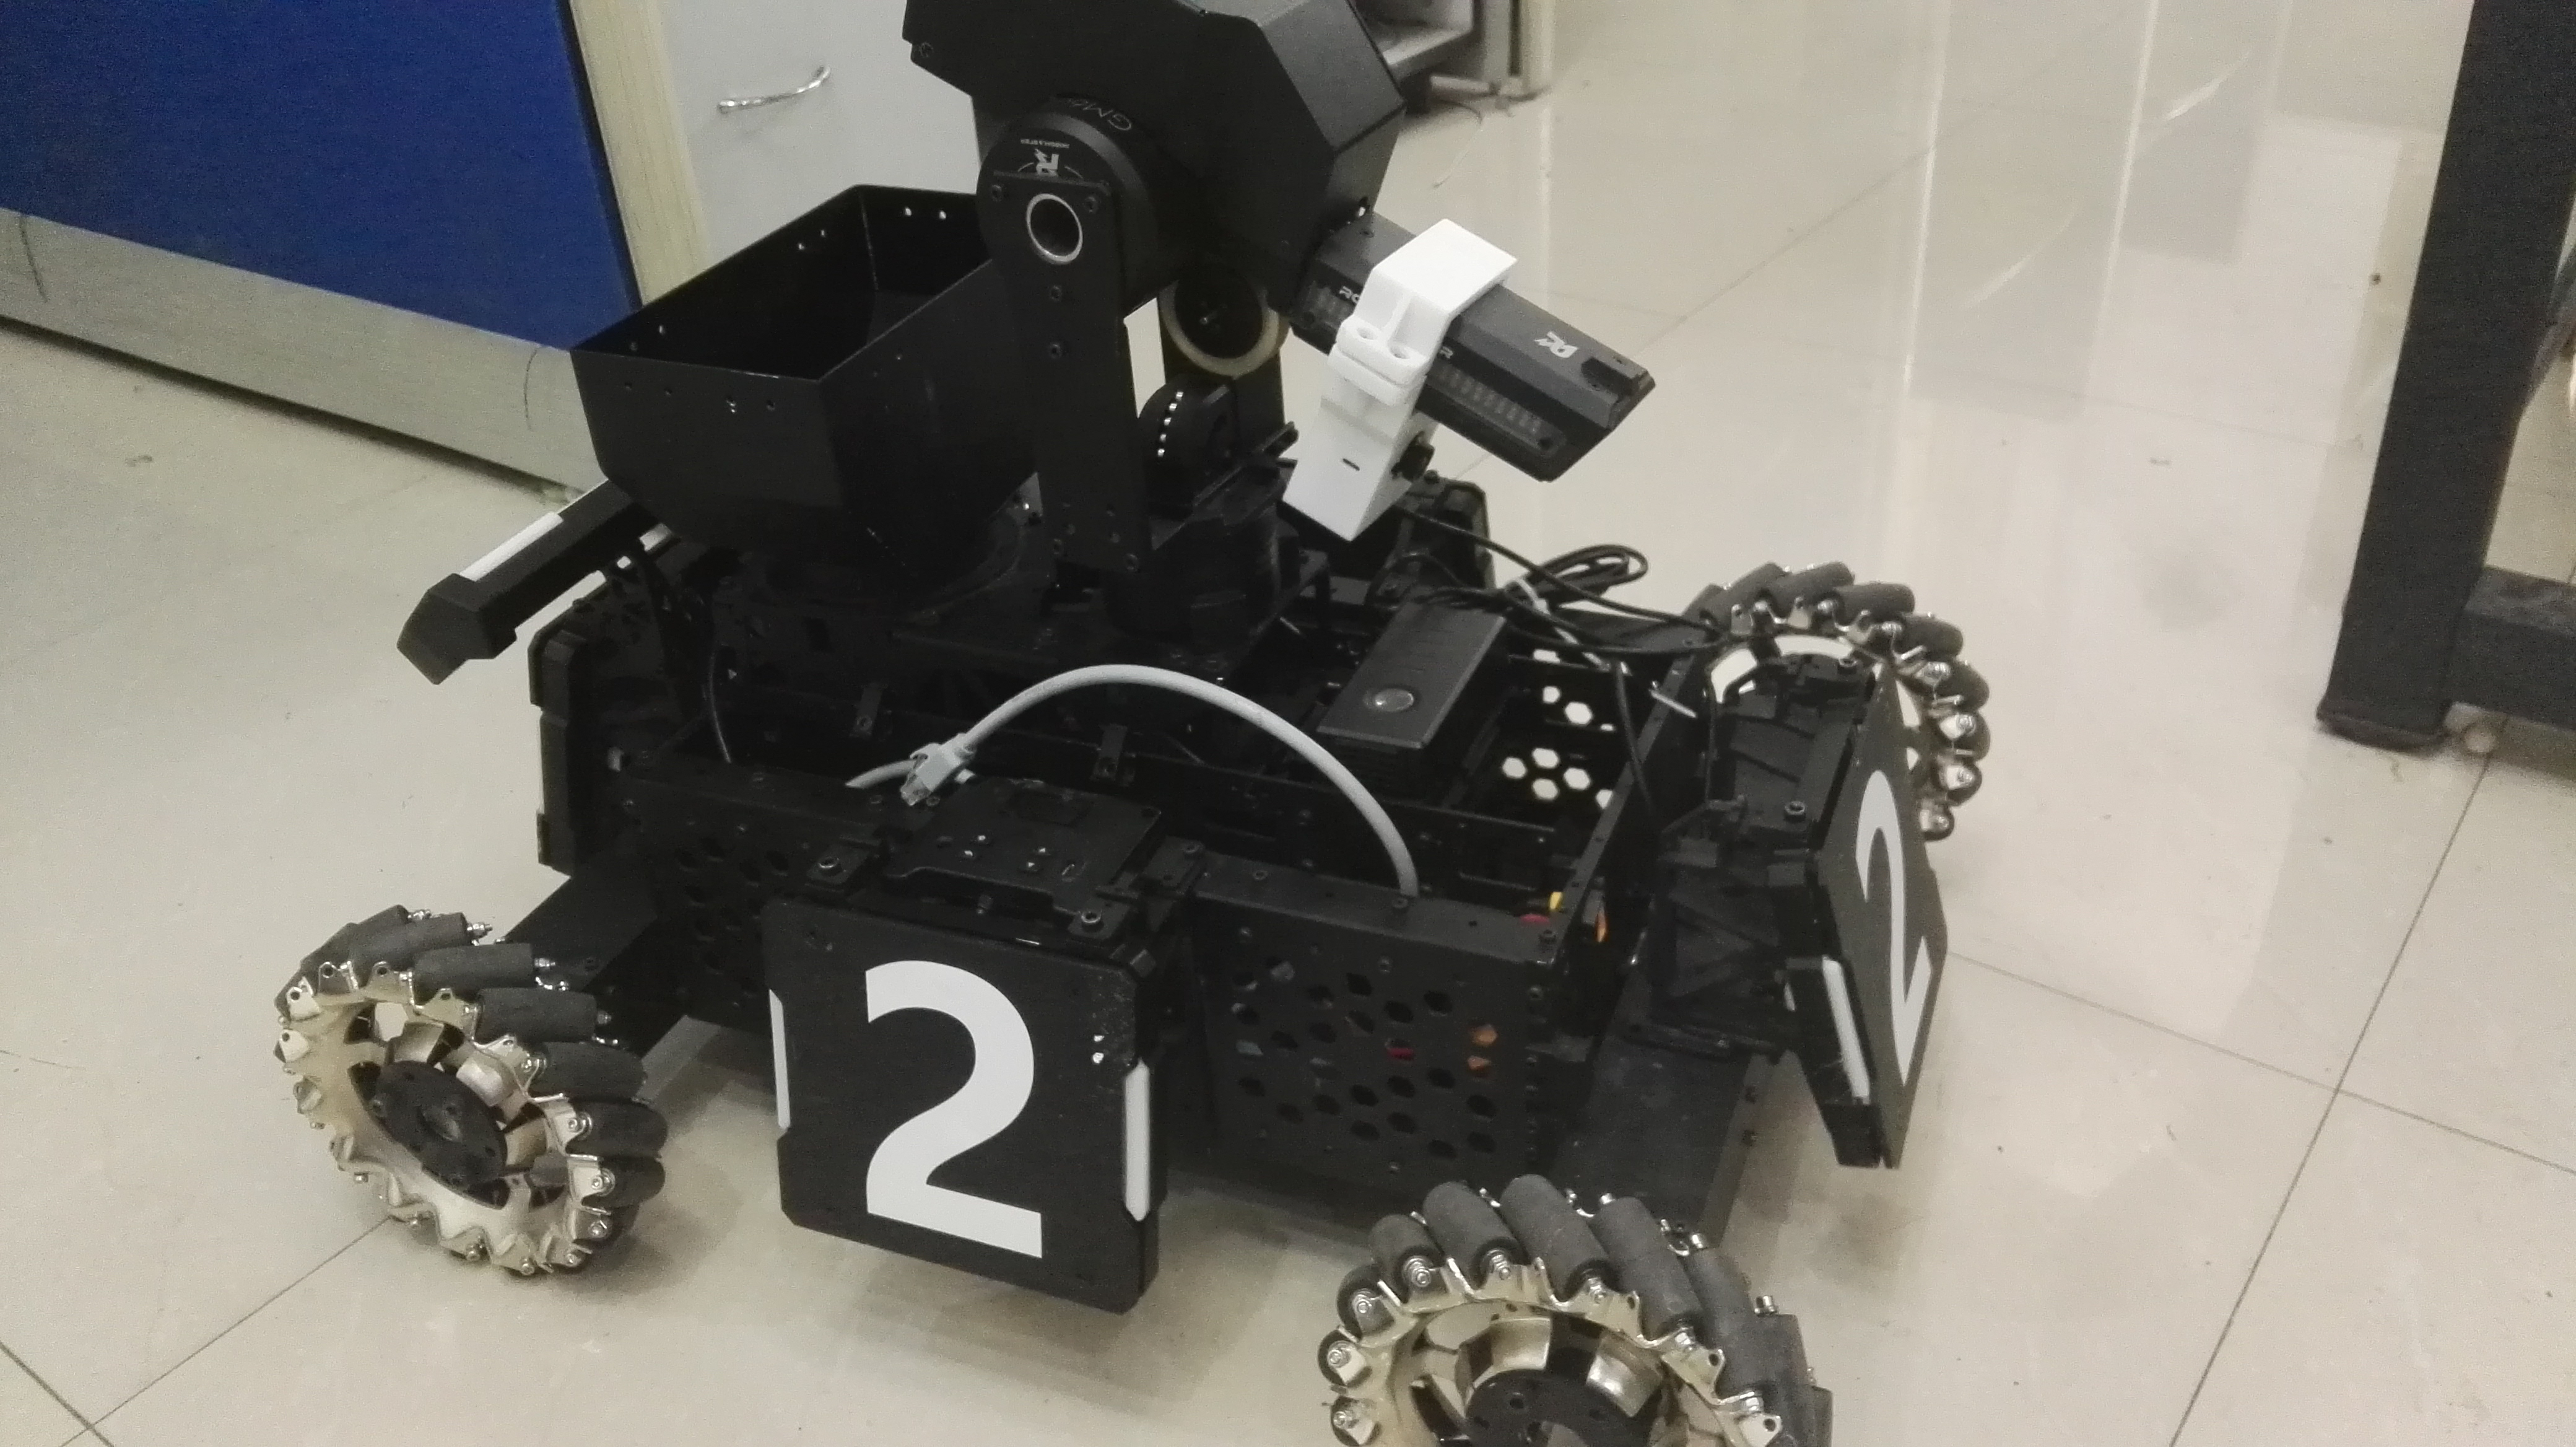
\includegraphics[width=0.80\textwidth]{figures/robot.jpg}
  \caption{轮式机器人实物}\label{realrobot}
\end{figure}

\section{奖励函数定义}
通过使用OpenAI gym标准的接口,实现ROS各个功能模组与决策系统的交互。通过串口向上位机发送轮式机器人的基本信息,轮式机器人智能体能够获得如比赛时间$t$、血量$h$、功率、里程计、速度、发射机构状态和遭受伤害的方向$d$等状态信息。通过传感器、定位算法(AMCL),轮式机器人智能体能够感知到自身位置与底盘偏航角$\left( x, y, \varphi \right)$。 通过目标识别算法(SSD-mobilenet),轮式机器人可以感知到敌人的位置$\left( x_e, y_e\right)$。

轮式机器人智能体所做出的动作包含下一步的目标位置与底盘偏航角$\left( x', y', \varphi' \right)$,或者相应的速度$\left( v_x, v_y, \omega \right)$,或加速度$\left( a_x, a_y, b \right)$,和发射机构云台的开火角度$\left( \theta, \psi \right)$。即云台俯仰角pitch、云台偏航角yaw。

考虑到与现有通信协议与控制算法整合,云台发射机构交由自动打击系统单独控制,打击策略为发现目标即开火,同时矫正云台姿态,智能体负责底盘运动的决策。最终定义状态$s$和动作$a$:
\begin{equation}
s = \left( x, y, \varphi, x_e, y_e, h, t, d \right),
\end{equation}
\begin{equation}
a = \left( x', y', \varphi' \right).
\end{equation}

奖励函数为:
\begin{equation}\label{reward}
r =
\begin{cases}
-1,  & \text{每受到一点伤害} \\
1, & \text{敌方轮式机器人出现在视野内} \\
10, & \text{获得增益buff}.
\end{cases}
\end{equation}

\section{代码设计}
\begin{figure}[ht]
  \centering
  % Requires \usepackage{graphicx}
  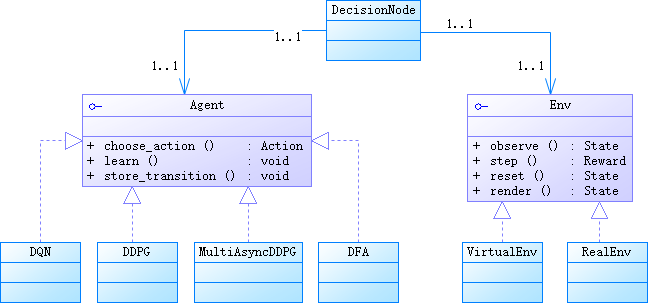
\includegraphics[width=\textwidth]{figures/classchart.png}
  \caption{轮式机器人决策系统类图}\label{classchart}
\end{figure}

\begin{figure}[ht]
  \centering
  % Requires \usepackage{graphicx}
  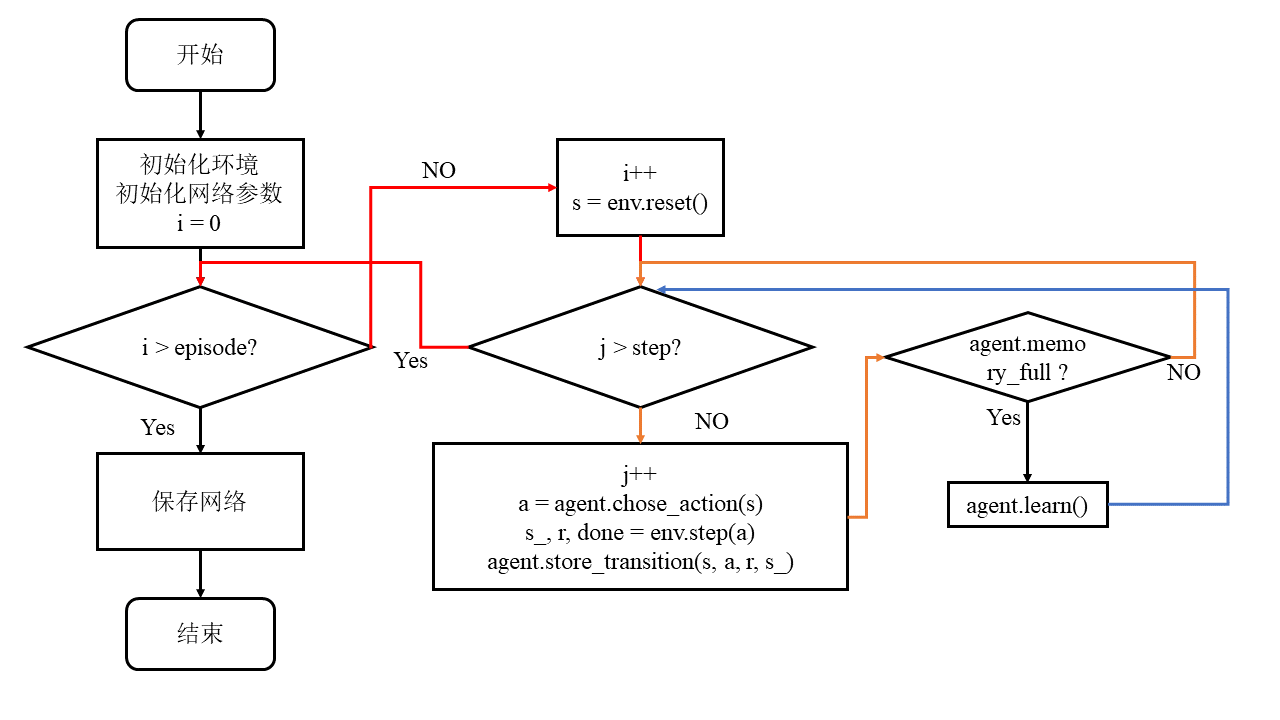
\includegraphics[width=\textwidth]{figures/flowchart.png}
  \caption{训练过程流程图}\label{flowchart}
\end{figure}

智能体类agent与环境类env结构与接口,如图\ref{classchart}所示。我们按照OpenAI gym接口规范标准,将智能体和与智能体直接交互的环境封装为接口。

环境类env隐藏了与轮式机器人感知、控制和通信等细节,从而使智能体类agent只需要关心与环境类env的交互,即接收一个状态$s$,做出相应的动作决策$a$。同时,智能体类agent隐藏了自主决策算法的训练和执行细节,环境类只需要关心执行智能体类输出的动作决策$a$。这样的结构允许我们在仿真环境到真实环境下的平滑过渡,同时也支持不同网络结构的深度强化学习算法的切换,甚至是使用非强化学习算法,如确定性有限状态机或遗传算法等启发式搜索算法。

针对深度强化学习,对于每一个情节(episode),我们设置最大步长数。训练时,轮式机器人智能体达到步长后即终止本次情节,重置环境,进入下一个情节的训练。训练过程如图\ref{flowchart}所示。

\subsection{Deep Q-learning}
使用Tensorflow构建DQN网络,网络结构如图\ref{dqnnet}所示。其中当前网络和目标网络均为三层全连接层神经网络,每层的神经元数分别为64,128,256,隐藏层的激活函数为Relu,输出层的激活函数为Tanh。
\begin{figure}[b]
  \centering
  % Requires \usepackage{graphicx}
  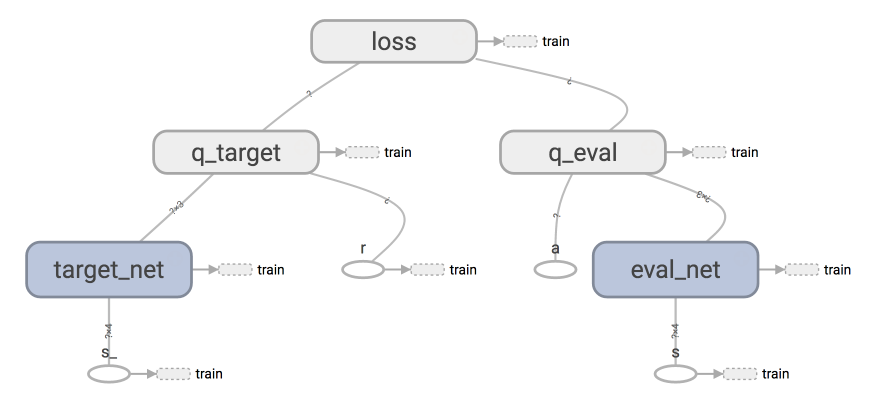
\includegraphics[width=0.80\textwidth]{figures/dqnnet.png}
  \caption{DQN网络结构图}\label{dqnnet}
\end{figure}

\subsection{Deep Deterministic Policy Gradient}
使用Tensorflow构建DDPG网络,网络结构如图\ref{ddpgnet}所示。其中当前网络和目标网络同构。网络中演员为三层全连接层神经网络,每层的神经元数分别为64,128,256,隐藏层的激活函数为Relu,输出层的激活函数为Tanh;评论家网络为三层全连接神经网络,每层的神经元数分别为64,128,1,输出标量评价值,即Q值的估计。
\begin{figure}[ht]
  \centering
  % Requires \usepackage{graphicx}
  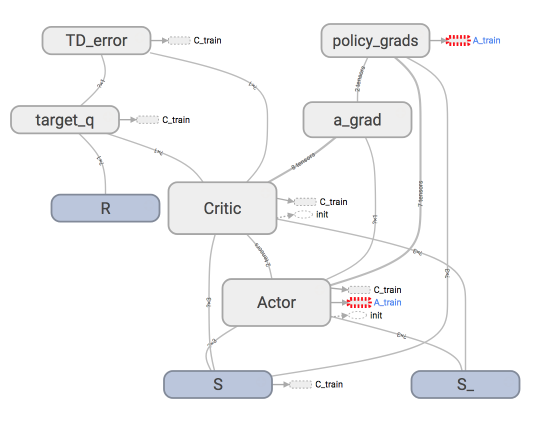
\includegraphics[width=0.80\textwidth]{figures/ddpgnet.png}
  \caption{DDPG网络结构图}\label{ddpgnet}
\end{figure}

\subsection{多智能体异步DDPG}
使用Tensorflow构建多智能体异步DDPG,其网络结构图与DDPG保持一致。在Gazebo仿真环境中,一次使用四台轮式机器人智能体进行对抗训练,如图\ref{multia}所示。
\begin{figure}[ht]
\centering
\subfigure{
\begin{minipage}[t]{0.40\linewidth}
\centering
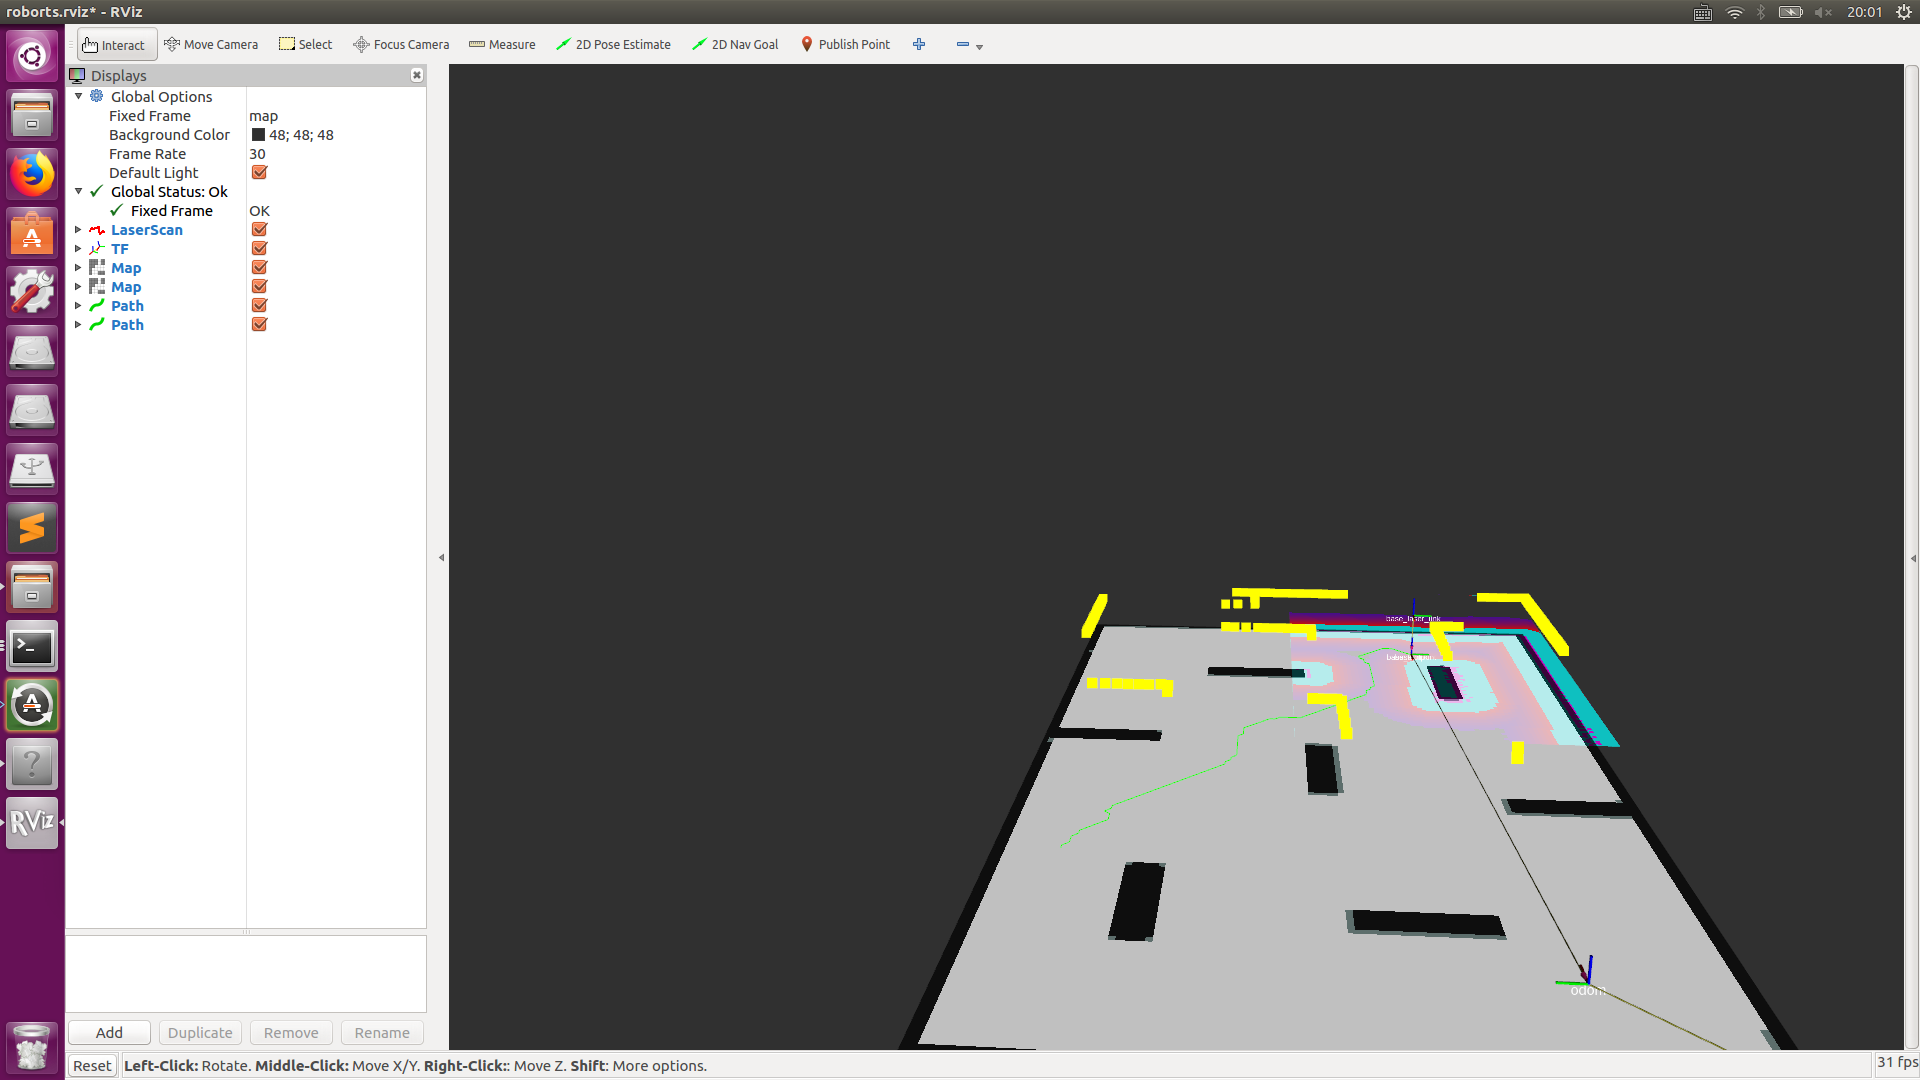
\includegraphics[width=2in]{rviz1.jpg}
\end{minipage}
}
\subfigure{
\begin{minipage}[t]{0.40\linewidth}
\centering
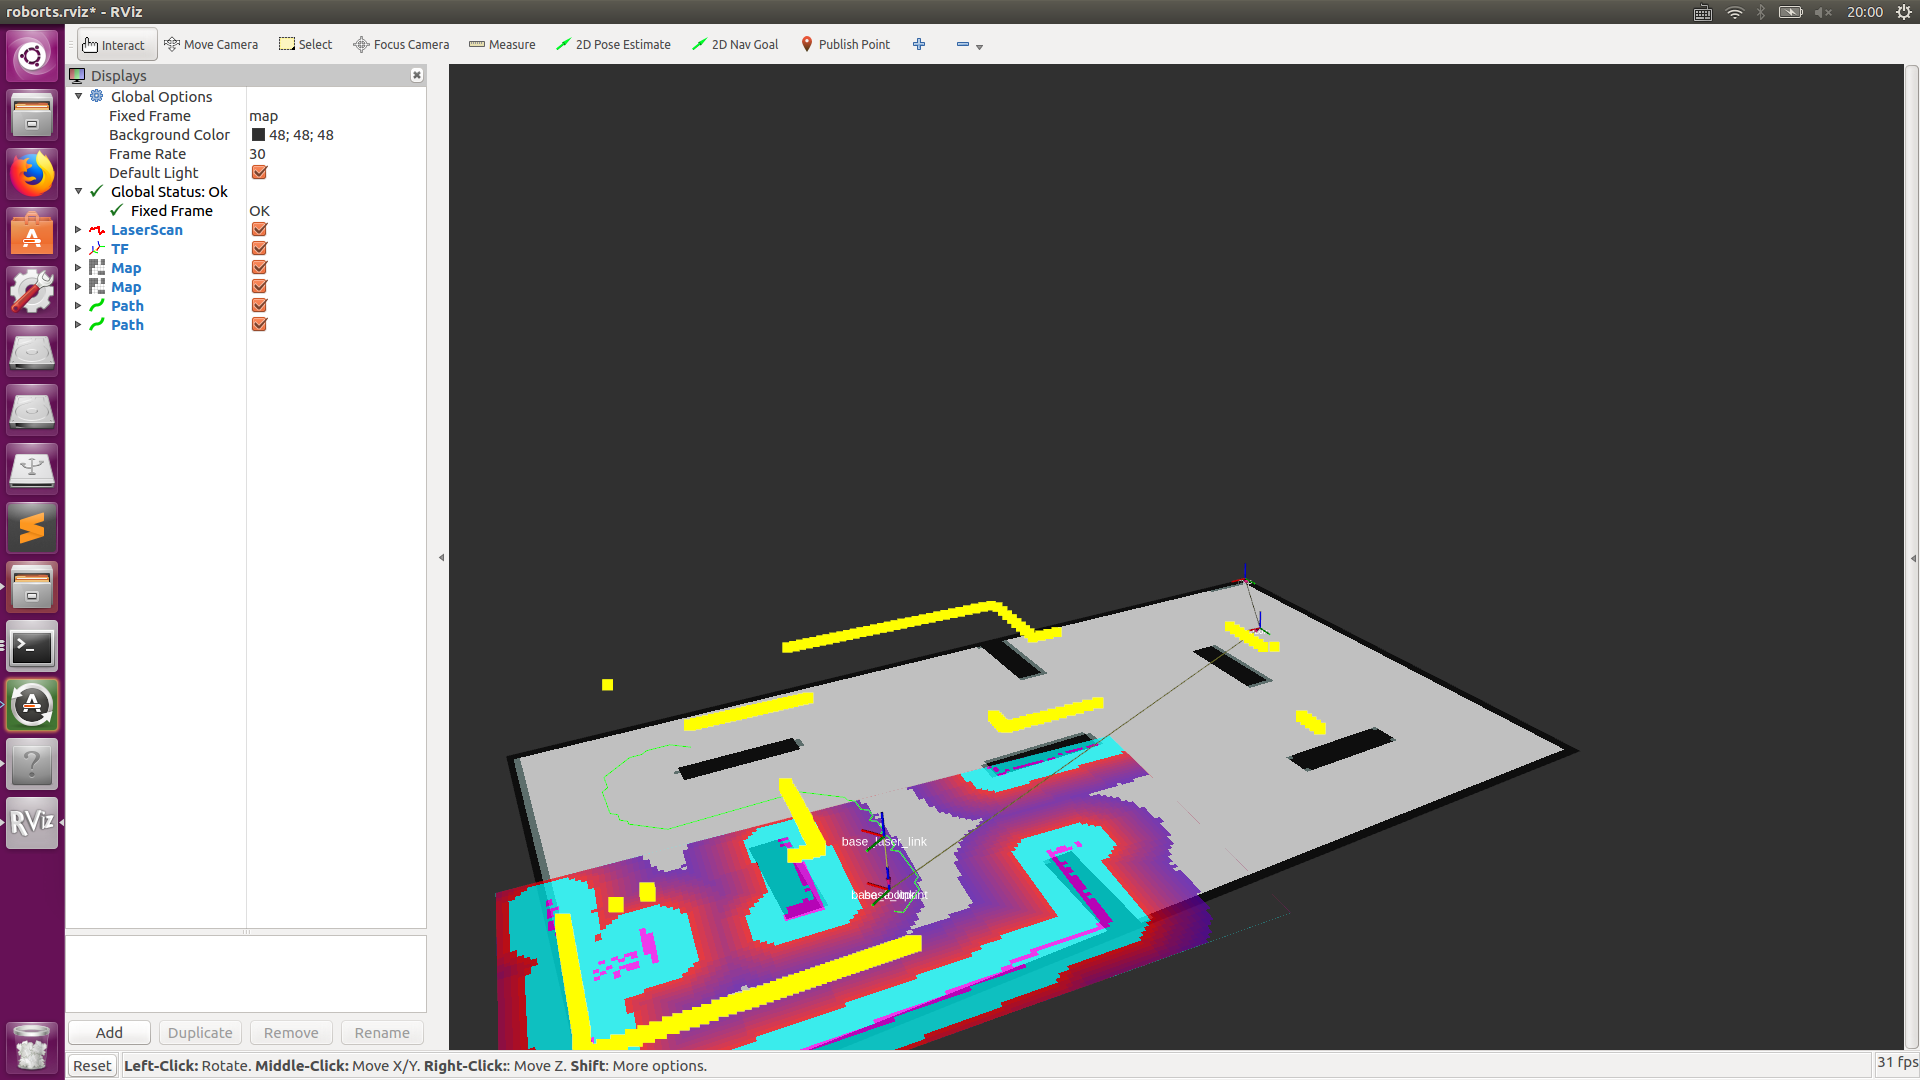
\includegraphics[width=2in]{rviz2.jpg}
\end{minipage}
}
\subfigure{
\begin{minipage}[t]{0.40\linewidth}
\centering
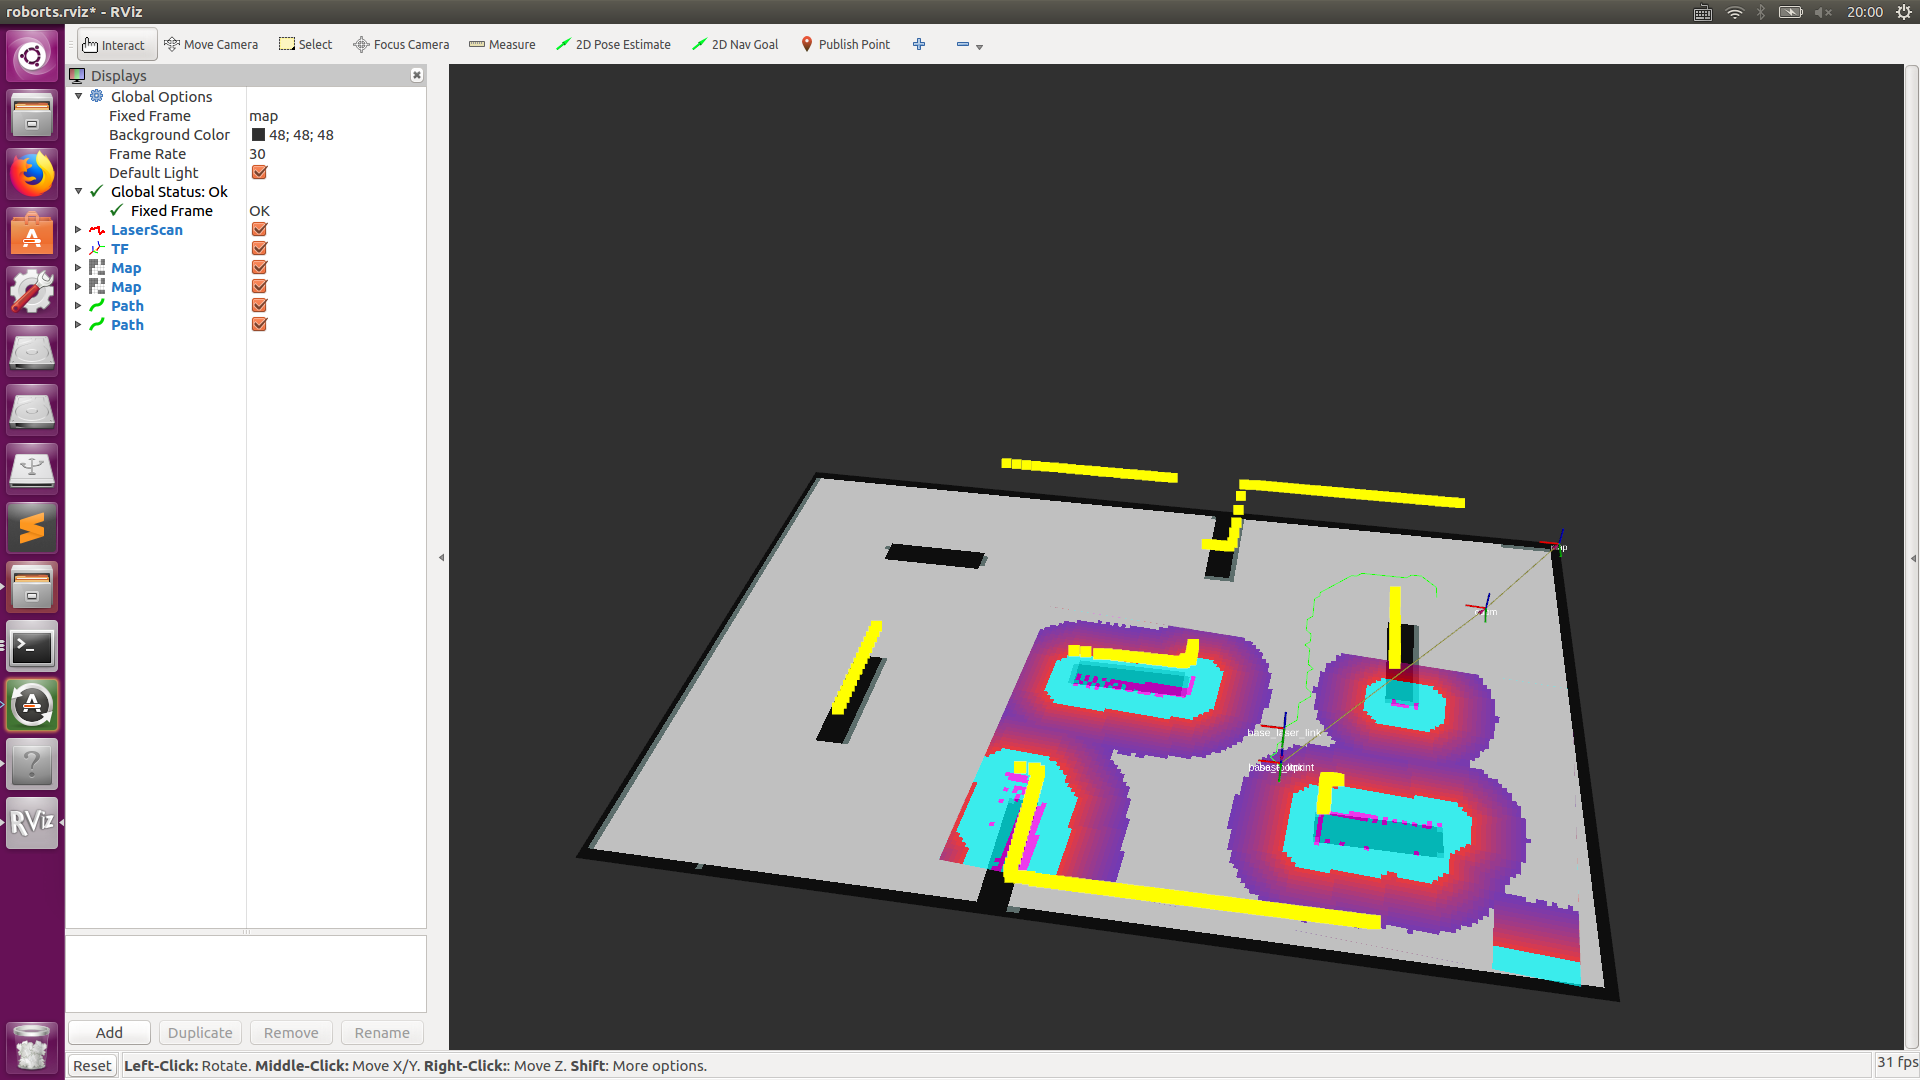
\includegraphics[width=2in]{rviz3.jpg}
\end{minipage}
}
\subfigure{
\begin{minipage}[t]{0.40\linewidth}
\centering
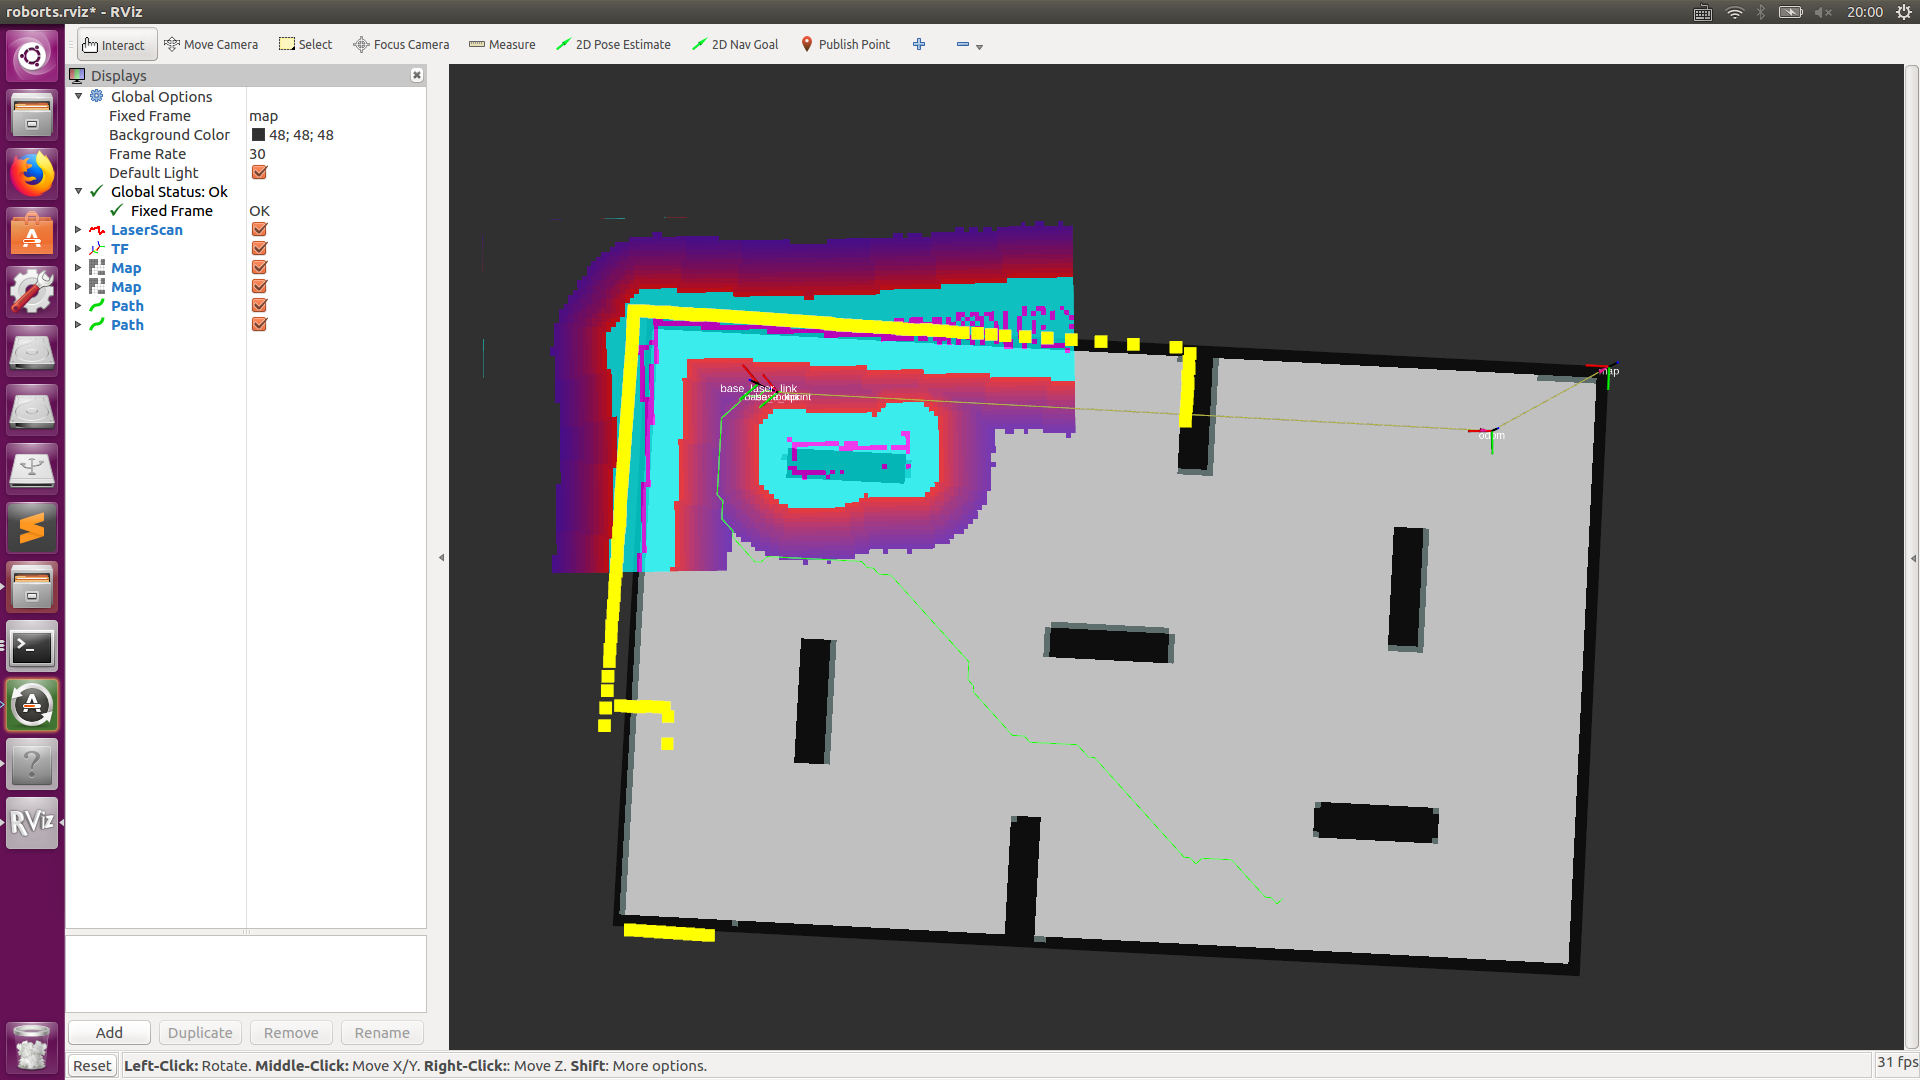
\includegraphics[width=2in]{rviz4.jpg}
\end{minipage}
}
\caption{多智能体异步DDPG训练}\label{multia}
\end{figure}

\section{实验结果}
\subsection{仿真实验结果}
在仿真环境下,我们使用上述定义的参数,应用DQN,DDPG,多智能体异步DDPG,在Gazebo仿真平台上训练全自主轮式机器人。使用的超参数有:
\begin{itemize}
  \item 情节数,episode:500。
  \item 最长步数,step:300。
  \item 折扣参数,$\gamma$:0.90。
  \item 学习率,learning rate:1e-3。
  \item 回放记忆长度,reply memory:30000。
  \item 批处理长度,batch size:50。
\end{itemize}

应用三种不同算法在仿真环境下的表现如图\ref{performance}所示。其中图\ref{accumulatedreward}表示仿真环境下轮式机器人在训练中共获得的奖励累加值,图\ref{averagereward}表示仿真环境下轮式机器人的步长平均奖励,即奖励累加值除以当前进行过的步长,可以是作为奖励期望的估计。由奖励设置式\ref{reward} 可推知,步长平均奖励近似于敌方出现在轮式机器人视野的概率,我们可将之称为锁定率。在图中我们可以看出,在DQN、DDPG 以及多智能体异步DDPG三种深度强化学习算法中,多智能体异步DDPG算法收敛速度较快,其模型锁定率能够达到18\%以上,而DDPG和DQN分别收敛在9\%和4\%左右。

\begin{figure}[hb]
  \centering
  % Requires \usepackage{graphicx}
  \subfigure[仿真环境下轮式机器人的累积奖励]{
  \label{accumulatedreward}
  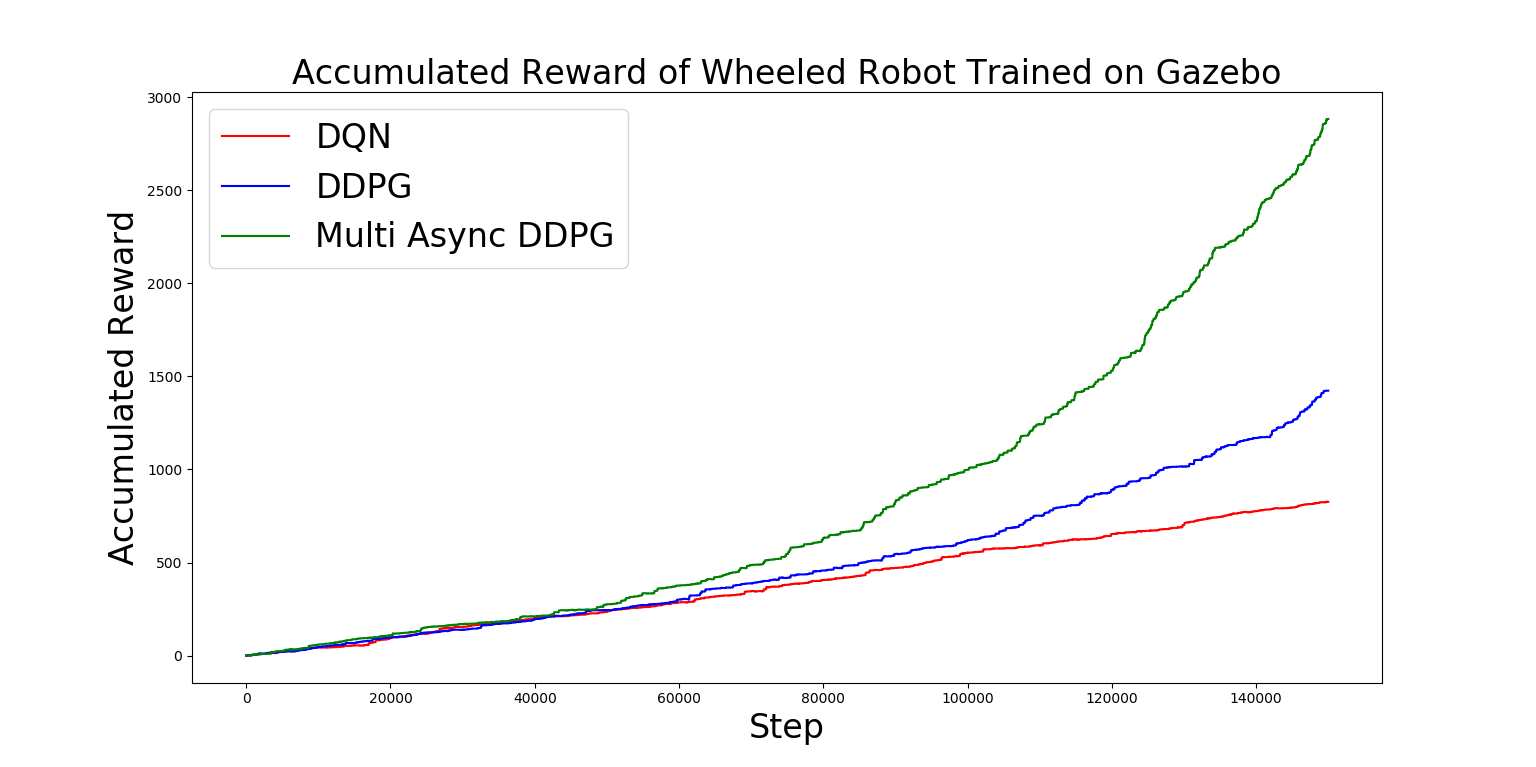
\includegraphics[width=0.80\textwidth]{figures/accumulatedreward.png}
  }
  \subfigure[仿真环境下轮式机器人的步长平均奖励]{
  \label{averagereward}
  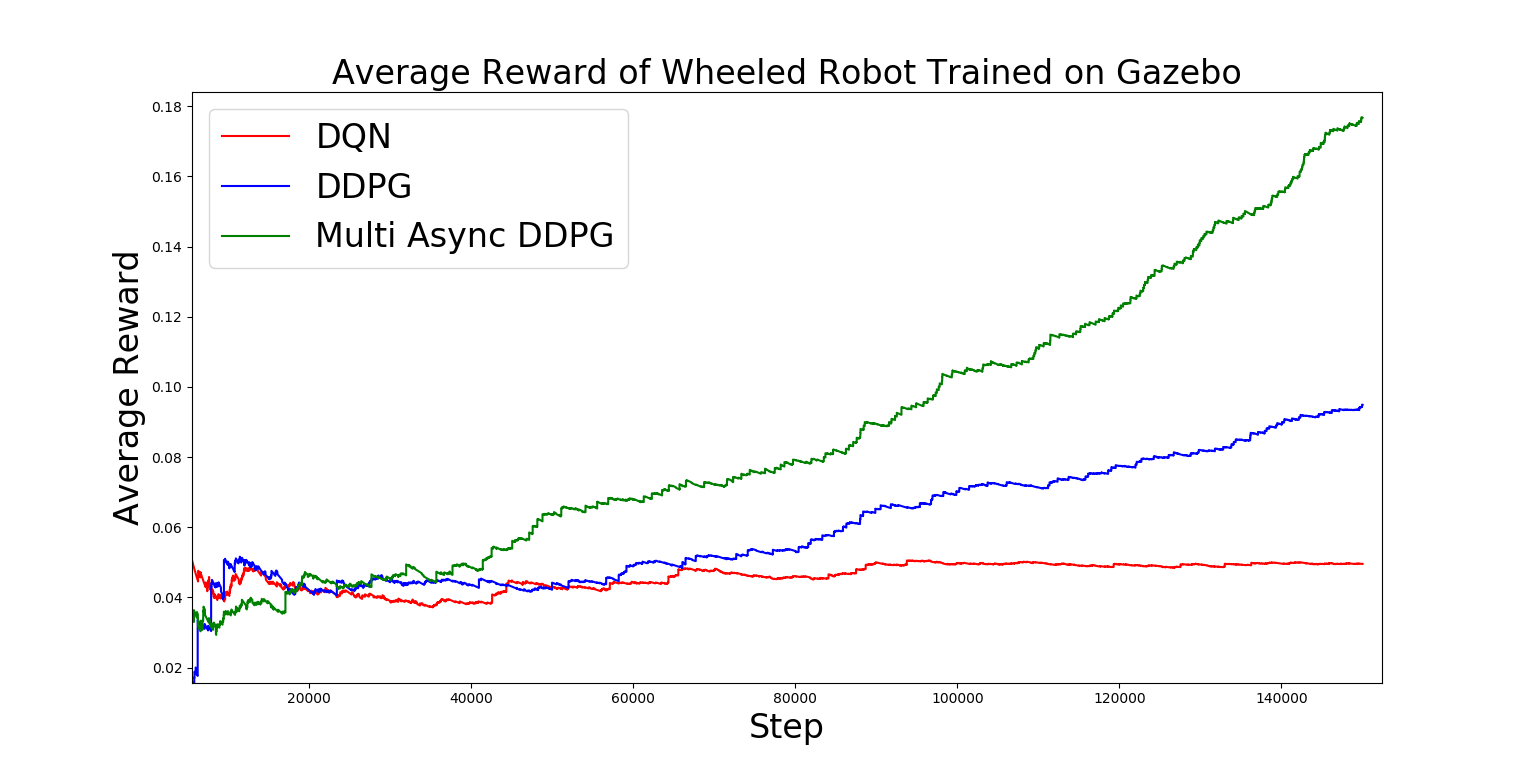
\includegraphics[width=0.80\textwidth]{figures/averagereward.png}
  }
  \caption{仿真环境下轮式机器人的训练表现}\label{performance}
\end{figure}

\subsection{真实环境下对抗结果}
在真实环境下,我们使用确定性有限状态机作为基线与三种不同算法训练的轮式机器人智能体各进行8次实际对战,在120s的比赛时间内的比赛结果如图\ref{result}所示。图中黑色直线为失败线,分布在黑色直线上的点即为血量被敌方轮式机器人伤害殆尽而结束比赛;棕色线为胜利线,分布在棕色线上的点即为在保佑一定血量的情况下使敌方轮式机器人血量消耗殆尽;橙色线为优势线,即在比赛时间结束时,敌我双方都没有击败对方,此时处于优势线右侧的点表示在比赛结束时,我方轮式机器人智能体保有血量高于敌方。
由图中结果可以发现多智能体异步DDPG算法和DDPG算法在真实环境下与敌方对抗时各有三次取得优势,实际上的表现相近,而DQN则很难取得优势。这说明了多智能体异步DDPG算法实际上是DDPG算法的快速收敛版。通过多智能体异步的方法部分克服了时延问题和采样速度较慢的问题。
\begin{figure}[ht]
  \centering
  % Requires \usepackage{graphicx}
  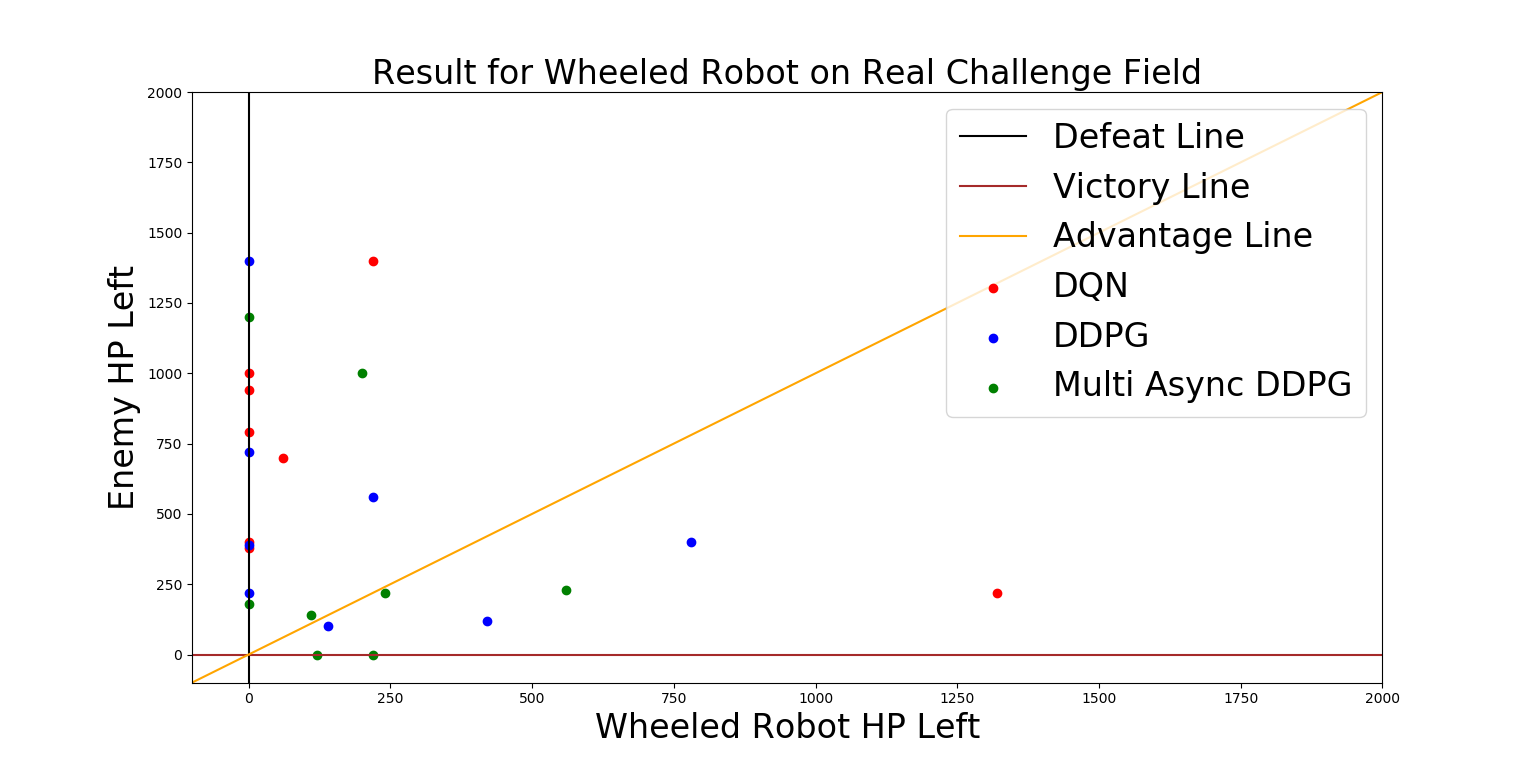
\includegraphics[width=0.80\textwidth]{figures/result.png}
  \caption{真实环境下轮式机器人对抗结果}\label{result}
\end{figure}


% 结论
%%%%%%%%%%%%%%%%%%%%%%%%%%%%%%%%%%%%%%%%%%%%%%%%%%%%%%%%%%%%%%%%%%%%%%%%%
%
%   LaTeX File for Doctor (Master) Thesis of Tsinghua University
%   LaTeX + CJK     清华大学博士(硕士)论文模板
%   Based on Wang Tianshu's Template for XJTU
%	Version: 1.00
%   Last Update: 2003-09-12
%
%%%%%%%%%%%%%%%%%%%%%%%%%%%%%%%%%%%%%%%%%%%%%%%%%%%%%%%%%%%%%%%%%%%%%%%%%
%   Copyright 2002-2003  by  Lei Wang (BaconChina)       (bcpub@sina.com)
%%%%%%%%%%%%%%%%%%%%%%%%%%%%%%%%%%%%%%%%%%%%%%%%%%%%%%%%%%%%%%%%%%%%%%%%%

\renewcommand{\baselinestretch}{1.5}
\fontsize{12pt}{13pt}\selectfont

\chapter{全文总结}\label{conclusion}
\markboth{全文总结}{全文总结}
%\addcontentsline{toc}{chapter}{\hei 总结与展望}
\section{全文总结}
深度强化学习已经准备好在AI领域掀起一场革命。深度强化学习向建立对于真实世界具有高水平理解能力的全自主系统迈出了坚实的一步。当前,深度学习使强化学习有能力处理先前极为棘手的问题。本文通过应用深度强化学习在轮式机器人上,以实现轮式机器人的全自主战斗决策。主要做的工作如下:
\vspace{-10pt}
\begin{enumerate}
  \item 基于ROS,构建了轮式机器人的决策系统。通过将智能体agent部分与环境env部分解耦,实现了决策系统的模块化。
  \item 简述了强化学习的基本原理,介绍了基于值函数与策略搜索的强化学习基本算法。
  \item 基于Gazebo,搭建了轮式机器人仿真平台。
  \item 提出了多智能体异步的训练方法,解决了真实环境下的时延问题和采样速度问题。
  \item 实现并检验了DQN、DDPG和多智能体异步DDPG在仿真环境和真实环境下的训练和表现。
\end{enumerate}

\section{对未来工作的展望}
根据本文的分析,可以发现深度强化学习已经广泛应用于机器人控制任务,从简单运动到复杂操作和全自主移动机器人控制。然而,强化学习在真实世界中的实际应用通常需要超出学习算法本身的大量额外工程:
\vspace{-10pt}
\begin{enumerate}
  \item 机器人无法感知到真实世界的全貌,即机器人只能部分感知当前状态。
  \item 真实世界往往是奖励稀疏的,如何确定奖励函数是一个棘手的问题。
  \item 机器人在真实环境下存在着感知、通信和控制时延,这还会使得机器人无法。
\end{enumerate}

在未来的工作中,应该着重与解决这些问题。建立基于部分部分可观测马尔可夫决策过程的模型和算法;应该设计基于状态-动作对概率分布的奖励函数,使连续的状态-动作空间都能收到奖励或者惩罚信号;使用并发和分布式的方法,克服机器人在真实世界中训练的时延。



%参考文献
\wuhao

%\bibliographystyle{unsrt}
\bibliographystyle{GBT7714-2005NLang}
%\ifpdf \phantomsection \fi

%\addcontentsline{toc}{chapter}{\hei 参考文献}
%\addtolength{\itemsep}{-0.8 em} % 缩小参考文献间的垂直间距, 在bibtex下无效
%\bibliography{reference/reference}

% 致谢

\clearpage
\phantomsection
\addcontentsline{toc}{chapter}{{\bf 参考文献}}
%\addtolength{\itemsep}{-0.5pt}  %修改参考文献间距

{\renewcommand\baselinestretch{1.25}\selectfont


\begin{thebibliography}{999}
\addtolength{\itemsep}{-1.05 em} % 缩小参考文献间的垂直间距
\setlength{\itemsep}{1pt}
%\renewcommand{\baselinestretch}{1.05}
\bibitem{1}
徐扬生. 智能机器人引领高新技术发展[J]. 企业科协, 2010 (9): 28-31.
\bibitem{2}
Christensen H I, Batzinger T, Bekris K, et al. A roadmap for us robotics: from internet to robotics[J]. Computing Community Consortium, 2009, 44.
\bibitem{3}
Salichs M A, Moreno L. Navigation of mobile robots: open questions[J]. Robotica, 2000, 18(3): 227-234.
\bibitem{4}
Beom H R, Cho H S. A sensor-based navigation for a mobile robot using fuzzy logic and reinforcement learning[J]. IEEE transactions on Systems, Man, and Cybernetics, 1995, 25(3): 464-477.
\bibitem{5}
Pandey A, Sonkar R K, Pandey K K, et al. Path planning navigation of mobile robot with obstacles avoidance using fuzzy logic controller[C]//2014 IEEE 8th International Conference on Intelligent Systems and Control (ISCO). IEEE, 2014: 39-41.
\bibitem{6}
Wang C, Soh Y C, Wang H, et al. A hierarchical genetic algorithm for path planning in a static environment with obstacles[C]//IEEE CCECE2002. Canadian Conference on Electrical and Computer Engineering. Conference Proceedings (Cat. No. 02CH37373). IEEE, 2002, 3: 1652-1657.
\bibitem{7}
Pandey A, Sonkar R K, Pandey K K, et al. Path planning navigation of mobile robot with obstacles avoidance using fuzzy logic controller[C]//2014 IEEE 8th International Conference on Intelligent Systems and Control (ISCO). IEEE, 2014: 39-41.
\bibitem{8}
Sutton R S, Barto A G. Introduction to reinforcement learning[M]. Cambridge: MIT press, 1998.
\bibitem{9}
LeCun Y. Yoshua Bengio, and Geoffrey Hinton[J]. Deep learning. nature, 2015, 521(7553): 436-444.
\bibitem{10}
Bengio Y, Courville A, Vincent P. Representation learning: A review and new perspectives[J]. IEEE transactions on pattern analysis and machine intelligence, 2013, 35(8): 1798-1828.
\bibitem{11}
Mnih V, Kavukcuoglu K, Silver D, et al. Human-level control through deep reinforcement learning[J]. Nature, 2015, 518(7540): 529.
\bibitem{12}
Silver D, Huang A, Maddison C J, et al. Mastering the game of Go with deep neural networks and tree search[J]. nature, 2016, 529(7587): 484.
\bibitem{13}
Levine S, Finn C, Darrell T, et al. End-to-end training of deep visuomotor policies[J]. The Journal of Machine Learning Research, 2016, 17(1): 1334-1373.
\bibitem{14}
Levine S, Pastor P, Krizhevsky A, et al. Learning hand-eye coordination for robotic grasping with deep learning and large-scale data collection[J]. The International Journal of Robotics Research, 2018, 37(4-5): 421-436.
\bibitem{15}
Duan Y, Schulman J, Chen X, et al. RL $^ 2$: Fast Reinforcement Learning via Slow Reinforcement Learning[J]. arXiv preprint arXiv:1611.02779, 2016.
\bibitem{16}
Wang J X, Kurth-Nelson Z, Kumaran D, et al. Prefrontal cortex as a meta-reinforcement learning system[J]. Nature neuroscience, 2018, 21(6): 860.
\bibitem{17}
Vinyals O, Ewalds T, Bartunov S, et al. Starcraft ii: A new challenge for reinforcement learning[J]. arXiv preprint arXiv:1708.04782, 2017.
\bibitem{18}
Kaelbling L P, Littman M L, Cassandra A R. Planning and acting in partially observable stochastic domains[J]. Artificial intelligence, 1998, 101(1-2): 99-134.
\bibitem{19}
Watkins C J C H, Dayan P. Q-learning[J]. Machine learning, 1992, 8(3-4): 279-292.
\bibitem{20}
Rummery G A, Niranjan M. On-line Q-learning using connectionist systems[M]. Cambridge, England: University of Cambridge, Department of Engineering, 1994.
\bibitem{21}
Koutník J, Cuccu G, Schmidhuber J, et al. Evolving large-scale neural networks for vision-based reinforcement learning[C]//Proceedings of the 15th annual conference on Genetic and evolutionary computation. ACM, 2013: 1061-1068.
\bibitem{22}
Deisenroth M P, Neumann G, Peters J. A survey on policy search for robotics[J]. Foundations and Trends® in Robotics, 2013, 2(1–2): 1-142.
\bibitem{23}
Williams R J. Simple statistical gradient-following algorithms for connectionist reinforcement learning[J]. Machine learning, 1992, 8(3-4): 229-256.
\bibitem{24}
Konda V R, Tsitsiklis J N. Onactor-critic algorithms[J]. SIAM journal on Control and Optimization, 2003, 42(4): 1143-1166.
\bibitem{25}
Schulman J, Moritz P, Levine S, et al. High-dimensional continuous control using generalized advantage estimation[J]. arXiv preprint arXiv:1506.02438, 2015.
\bibitem{26}
Lillicrap T P, Hunt J J, Pritzel A, et al. Continuous control with deep reinforcement learning[J]. arXiv preprint arXiv:1509.02971, 2015.
\bibitem{27}
Gu S, Holly E, Lillicrap T, et al. Deep reinforcement learning for robotic manipulation with asynchronous off-policy updates[C]//2017 IEEE international conference on robotics and automation (ICRA). IEEE, 2017: 3389-3396.
\bibitem{28}
Van Hasselt H, Guez A, Silver D. Deep reinforcement learning with double q-learning[C]//Thirtieth AAAI Conference on Artificial Intelligence. 2016.
\bibitem{29}
Wang Z, Schaul T, Hessel M, et al. Dueling network architectures for deep reinforcement learning[J]. arXiv preprint arXiv:1511.06581, 2015.
\bibitem{30}
Schaul T, Quan J, Antonoglou I, et al. Prioritized experience replay[J]. arXiv preprint arXiv:1511.05952, 2015.
\end{thebibliography}

%%%%%%%%%%%%%%%%%%%%%%%%%%%%%%%%%%%%%%%%%%%%%%%%%%%%%%%%%%%%%%%%%%%%%%%%%
%
%   LaTeX File for Doctor (Master) Thesis of Tsinghua University
%   LaTeX + CJK     清华大学博士(硕士)论文模板
%   Based on Wang Tianshu's Template for XJTU
%   Version: 1.00
%   Last Update: 2003-09-12
%
%%%%%%%%%%%%%%%%%%%%%%%%%%%%%%%%%%%%%%%%%%%%%%%%%%%%%%%%%%%%%%%%%%%%%%%%%
%   Copyright 2002-2003  by  Lei Wang (BaconChina)       (bcpub@sina.com)
%%%%%%%%%%%%%%%%%%%%%%%%%%%%%%%%%%%%%%%%%%%%%%%%%%%%%%%%%%%%%%%%%%%%%%%%%


%%%%%%%%%%%%%%%%%%%%%%%%%%%%%%%%%%%%%%%%%%%%%%%%%%%%%%%%%%%%%%%%%%%%%%%%%
%
%   LaTeX File for phd thesis of xi'an Jiao Tong University
%
%%%%%%%%%%%%%%%%%%%%%%%%%%%%%%%%%%%%%%%%%%%%%%%%%%%%%%%%%%%%%%%%%%%%%%%%%
%   Copyright 2002  by  Wang Tianshu    (tswang@asia.com)
%%%%%%%%%%%%%%%%%%%%%%%%%%%%%%%%%%%%%%%%%%%%%%%%%%%%%%%%%%%%%%%%%%%%%%%%%
\renewcommand{\baselinestretch}{1.5}
\fontsize{12pt}{13pt}\selectfont

\chapter*{致~~~~谢}
\markboth{致谢}{致谢}
\addcontentsline{toc}{chapter}{\hei 致谢}
首先要感谢我的毕业设计指导老师史豪斌副教授。论文是在史老师的悉心指导下完成的。在论文的进展中,史老师提供了实验平台和学习资料,在学业和论文写作上提出了许多宝贵意见。史老师严谨的治学态度以及丰富的实践经验将是我以后学习和工作的动力和楷模。在此谨向我的指导老师史豪斌副教授表示衷心的感谢。

同时要感谢西北工业大学竞技机器人基地的同学和队友们,是我们一起共同的努力,让我们能在ICRA的平台上进行机器人与人工智能的竞技和挑战。



\chapter*{毕业设计小结}
\markboth{毕业设计小结}{毕业设计小结}
\addcontentsline{toc}{chapter}{\hei 毕业设计小结}
这次毕业设计是对我四年本科学习的一个总结,涉及了机器人感知、控制与通信,深度神经网络与深度强化学习,这对我来说是一个全面的考验。虽然在过去的比赛中经常接触和使用仿真环境Gazebo以及机器人操作系统ROS,但是对它们的理解并不算透彻。在这次毕业设计的过程中,我又系统地学习了ROS,深刻理解了ROS消息机制。对于深度神经网络方面,我在这次的毕业设计实践中感受数学工具在开辟新算法和思路时的重要性以及扎实的打好数学基础对于计算机相关专业学习的重要性。

通过本次毕业设计,我对深度强化学习在轮式机器人上的应用有了更深入的了解,对今后研究生阶段的学习和奋斗的目标也更加明确。






%  附录

%\begin{appendix}
%    \renewcommand{\chaptername}{附录\Alph{chapter}}
%   \chapter*{附~~录}
\markboth{附录}{附录}
\addcontentsline{toc}{chapter}{\hei 附录}
\noindent\bfseries\texttt{test.py}源代码:
\setmonofont{Monaco}
\lstset{basicstyle=\ttfamily\scriptsize,keywordstyle=\color{blue},commentstyle=\color{green},stringstyle=\color{red},tabsize=4,frameround=fttt,escapeinside=``,lineskip=0.6pt}
\begin{lstlisting}[language=Python]
#!/usr/bin/env python
from TOSSIM import *
from random import *
import sys

if len(sys.argv) < 3:
	print "usage: need 2 parameter, nodes number and simulate time"
	sys.exit(0)

nodes = int(sys.argv[1])
sim_time = int(sys.argv[2])
t = Tossim([])
r = t.radio()

f = open("topo.txt", "r")
lines = f.readlines()
for line in lines:
  s = line.split()
  if (len(s) > 0):
    if s[0] == "gain":
      r.add(int(s[1]), int(s[2]), float(s[3]))

noise = open("meyer-short.txt", "r")
lines = noise.readlines()
for line in lines:
  str = line.strip()
  if (str != ""):
    val = int(str)
    for i in range(0, nodes):
      m = t.getNode(i);
      m.addNoiseTraceReading(val)

for i in range(0, nodes):
  m = t.getNode(i);
  m.createNoiseModel();
  time = randint(t.ticksPerSecond(), 10 * t.ticksPerSecond())
  m.bootAtTime(time)
  print "Booting ", i, " at time ", time

print "Starting simulation."

t.addChannel("Forwarder", sys.stdout)
t.addChannel("TestNetworkC", sys.stdout)
t.addChannel("TreeRouting", sys.stdout)
t.addChannel("LI", sys.stdout)

while (t.time() < sim_time):
  t.runNextEvent()

print "Completed simulation."
\end{lstlisting}

\noindent\bfseries\texttt{ctpsim-3d.py}源代码:
\begin{lstlisting}[language=Python,tabsize=2]
#!/usr/bin/env python
import xmlrpclib,time
import re

nodes = 10
server = xmlrpclib.Server('http://localhost:20738/RPC2')
G = server.ubigraph

G.clear()

node = [0 for col in range(nodes)]

for i in range(0,nodes):
	node[i] = G.new_vertex()
	G.set_vertex_attribute(node[i], 'label', str(i))
	G.set_vertex_attribute(node[i], 'shape','sphere')
	G.set_vertex_attribute(node[i], 'size','0.5')
	G.set_vertex_attribute(node[i], 'color','#1E90FF')

edge = [[0 for col in range(nodes)] for row in range(nodes)]

for i in range(0,nodes):
	for j in range(i+1, nodes):
		edge[i][j] = G.new_edge(node[i], node[j])
		edge[j][i] = edge[i][j]

topo = open('topo.txt', 'r')
lines = topo.readlines()
for line in lines:
	s = line.split()
	if s[0] == 'gain':
		if int(s[1]) < nodes and int(s[2]) < 
				nodes and int(s[1]) < int(s[2]):
			G.set_edge_attribute(edge[int(s[1])][int(s[2])],
					     'strength',
					     str(1 + float(s[3]) / 120.0))
			#G.set_edge_attribute(edge[int(s[1])][int(s[2])],
					      'label', s[3]) # add gain value

G.set_vertex_attribute(node[0], 'color', '#FFFF00') # root node

def node_spark(node_id):
	node_id = int(node_id)
	G.set_vertex_attribute(node[node_id], 'color', '#FF0000')
	G.set_vertex_attribute(node[node_id], 'color', '#FFFFFF')
	G.set_vertex_attribute(node[node_id], 'color', '#FF0000')
	G.set_vertex_attribute(node[node_id], 'color', '#FFFFFF')
	if node_id != 0:
		G.set_vertex_attribute(node[node_id], 'color', '#1E90FF')
	else:
		G.set_vertex_attribute(node[node_id], 'color', '#FFFF00')


def node_display_debug_str(node_id, debug_str):
	G.set_vertex_attribute(node[int(node_id)], 'label', node_id+": "+debug_str)
	#time.sleep(0.0)
	#G.set_vertex_attribute(node[node_id], 'label', str(node_id))

def process_boot_at_time(node_id, time):
	G.set_vertex_attribute(node[int(node_id)], 'label','boot at:'+time)


def process_parent_change(node_id, origin_parent, new_parent):
	node_id = int(node_id)
	origin_parent = int(origin_parent)
	new_parent = int(new_parent)
	if origin_parent != 65535:
		G.set_edge_attribute(edge[node_id][origin_parent], 'color', '#C0C0C0')
		G.set_edge_attribute(edge[node_id][origin_parent], 'width','1')
	G.set_edge_attribute(edge[node_id][new_parent], 'color', '#FF00FF')
	G.set_edge_attribute(edge[node_id][new_parent], 'width','7')
	time.sleep(0.5)

def animateArrow(e, reverse):
  pos = 0.0
  if reverse:
    pos = 1.0
  G.set_edge_attribute(e, "arrow_position", str(pos))
  G.set_edge_attribute(e, "arrow_reverse", str(reverse))
  G.set_edge_attribute(e, "arrow", "true")
  for i in range(0,20):
    a = i / 19.0
    if reverse:
      a = 1.0 - a
    G.set_edge_attribute(e, "arrow_position", str(a))
    time.sleep(0.05)
  G.set_edge_attribute(e, "arrow", "false")

def animate_broadcast(node_id):
	node_id = int(node_id)
	for j in range(2):
		for i in range(21):
			G.set_vertex_attribute(node[node_id], 
				'size', str(0.5 + i / 20.0))
		for i in range(21):
			G.set_vertex_attribute(node[node_id],
				'size', str(0.5 + (20 - i)/20.0))

def process_send_beacon(node_id):
	node_id = int(node_id)
	animate_broadcast(node_id)
	

def process_forwoard_subsend(node_id, dest):
	print node_id, dest
	node_id = int(node_id)
	dest = int(dest)
	if node_id == dest:
		return
	G.set_edge_attribute(edge[node_id][dest], 'arrow','true')
	if node_id > dest:
		G.set_edge_attribute(edge[node_id][dest], "arrow_reverse", 'true')
	speed = 10 # the smaller, the faster
	for pos in range(speed+1):
			if node_id < dest:
				G.set_edge_attribute(edge[node_id][dest], 
					"arrow_position", str(pos / float(speed)))
			else:
				G.set_edge_attribute(edge[node_id][dest], 
					"arrow_position", str(1- pos / float(speed)))
			time.sleep(0.05)
	G.set_edge_attribute(edge[node_id][dest], "arrow_reverse", 'false')
	G.set_edge_attribute(edge[node_id][dest], 'arrow','false')

def dispatch_each_line(line):
	re_boot_at_time = r'Booting  (/d+)  at time  (/d+)'
	re_debug = r'^DEBUG \((\d+)\): (.*)'

	re_parent_change = r'Changed parent. from (\d+) to (\d+)'
	# 1.parent,  2.etx
	re_send_beacon = r'CtpRoutingEngineP\$0\$sendBeaconTask\$runTask parent: (\d+) etx: (\d+)' 
	# 1.dest, 2. error
	re_forward_subsend = r'CtpForwardingEngineP\$0\$SubSend\$sendDone to (\d+) and (\d+)' 

	match = re.match(re_boot_at_time, line)
	if match:
		process_boot_at_time(match.group(1), match.group(2))
	else:	# match debug messages
		match = re.match(re_debug, line)
		if match:
			node_id = match.group(1)
			node_spark(node_id)
			debug_str = match.group(2)
			node_display_debug_str(node_id, debug_str)
			
			if re.match(re_parent_change, debug_str):
				match = re.match(re_parent_change, debug_str)
				process_parent_change(node_id, match.group(1), match.group(2))
			elif re.match(re_send_beacon, debug_str):
				process_send_beacon(node_id)
			elif re.match(re_forward_subsend, debug_str):	# Forwarder send a packet
				match = re.match(re_forward_subsend, debug_str)
				process_forwoard_subsend(node_id, match.group(1))
line = raw_input()
while line:
	dispatch_each_line(line)
	line = raw_input()
\end{lstlisting}

%\end{appendix}

% 发表的文章列表

%\include{appendix/publications}

\clearpage
\end{document}

%%%%%%%%%%%%%%%%%% End of the file  %%%%%%%%%%%%%%%%%%%%%%%%
